\documentclass[a4paper,11pt,oneside]{book}
\usepackage{alphabeta}

\usepackage{multirow}
\usepackage[utf8]{inputenc}
\usepackage[table]{xcolor}
\usepackage{graphicx}
\usepackage{geometry}
\usepackage{adjustbox}
\usepackage{changepage}
\usepackage{hyperref}
\usepackage{pdfpages}
\usepackage{titlesec}
\usepackage{longtable}

\usepackage{minted}
\usemintedstyle{manni}

\titleformat{\chapter}[display]
{\normalfont\Huge\bfseries}
{\thesection.}{0.5em}{}
\titleformat{\section}[display]
{\normalfont\huge\bfseries}
{\thesection.}{0.5em}{}
\titleformat{\subsection}[display]
{\normalfont\Large\bfseries}
{\thesection.}{0.5em}{}

%---------------------------------
% COLORI

\definecolor{bondiblue}{rgb}{0.0, 0.58, 0.71}
\definecolor{awesome}{rgb}{1.0, 0.13, 0.32}
\definecolor{darkspringgreen}{rgb}{0.09, 0.45, 0.27}
\definecolor{darktangerine}{rgb}{1.0, 0.66, 0.07}
\definecolor{emerald}{rgb}{0.31, 0.78, 0.47}
\definecolor{ferrarired}{rgb}{1.0, 0.11, 0.0}
\definecolor{denim}{rgb}{0.08, 0.38, 0.74}
\definecolor{cerise}{rgb}{0.87, 0.19, 0.39}
\definecolor{chromeyellow}{rgb}{1.0, 0.65, 0.0}
\definecolor{electriccrimson}{rgb}{1.0, 0.0, 0.25}
\definecolor{lapislazuli}{rgb}{0.15, 0.38, 0.61}
\definecolor{opal}{rgb}{0.66,0.76,0.74}

%---------------------------------


\hypersetup{
    colorlinks=true,
    linkcolor=black,
    filecolor=magenta,      
    urlcolor=red,
    pdftitle={BOPO},
    pdfpagemode=FullScreen,
    }


\geometry{a4paper,top=3cm,bottom=3cm,left=3.5cm,right=3.5cm}
\linespread{1}
\setlength{\arrayrulewidth}{0.5mm}
\setlength{\tabcolsep}{20pt}
\renewcommand{\arraystretch}{1.8}
\renewcommand{\contentsname}{Indice}
 
\pagestyle{empty}

\begin{document}

\thispagestyle{empty}
\vspace{2cm}

\begin{center}                                                            
    \vspace{5mm}
    {\LARGE UNIVERSIT\`A DI BOLOGNA} \\                       
      \vspace{2cm}
\end{center}
\begin{center}
  
\includegraphics[scale=0.1]{figs/bopo.png}
  \vspace{1 cm}
\LARGE\textbf{\\Backup Orchestrator \\Package Organizer} \\                       
\end{center}

\begin{flushleft}
    \vspace{3cm}
      {\Large{Sviluppato da:}}\\
      \vspace{3mm}
      \textbf{\@ Daniele Nanni Cirulli}\\
      \vspace{1mm}
      \textbf{\@ Lorenzo Venerandi}\\
      \vspace{1mm}
      \textbf{\@ Patrick Di Fazio}\\
\end{flushleft}        %capoverso allineato a destra
\begin{center}
\vfill
      {\large Anno accademico \@2021/2022} \\
\end{center}

\newpage
\tableofcontents

\chapter*{Abstract}
\addcontentsline{toc}{chapter}{Abstract}

Il progetto consiste nella realizzazione di un servizio di 
memorizzazione su cloud che permette agli utenti registrati e 
autenticati di accedere alla propria area di archiviazione, dove sarà 
possibile gestire i propri dati. Inoltre ogni utente avrà la 
possibilità di unirsi ad uno o più gruppi, potendo accedere ai file 
condivisi dai membri di questi ultimi.
L’applicazione predispone funzionalità come organizzazione di file per 
nome, dimensione , data di caricamento e altre tipologie di filtro e 
la visualizzazione sarà gestita attraverso delle sezioni che potranno 
essere personalizzate dall’utente.
\pagebreak

\chapter*{Analisi dei requisiti}
\addcontentsline{toc}{chapter}{\textbf{Analisi dei requisiti}}

\phantomsection
\section*{Raccolta dei Requisiti}
\addcontentsline{toc}{section}{Raccolta dei requisiti}

\begin{itemize}

  \item L'utente deve potersi registrare, fornendo username e password.
  
  \item L'utente può accedere al portale utilizzando le credenziali con cui si è registrato (username e password).
  
  \item Ogni utente avrà a disposizione il suo spazio di archiviazione personale, con una dimensione massima di 1 Gb.
  
  \item L'utente ha la possibilità di caricare e scaricare file, rinominarli ed eliminarli.
  
  \item È presente un amministratore che può gestire gli utenti e approvare o declinare la richiesta di creazione dei gruppi.
  
  \item È presente una sezione dedicata ai gruppi, dove è possibile partecipare ad uno o più gruppi.
  
  \item Ogni utente può far parte di al massimo N gruppi.
  
  \item Ogni utente avrà la possibilità di accedere ad una sezione di
  personalizzazione, dove potrà creare le proprie viste a seconda delle cose che vuole visualizzare, per esempio ordine alfabetico, dimensione, etc...
  
  \item Sarà possibile utilizzare le viste create nella sezione di personalizzazione nell'area personale.
  
  \item L'utente avrà a disposizione degli strumenti per gestire il suo account ( cambio password, ... ).
  
  \item Il proprietario del servizio deve mettere a disposizione uno spazio di archiviazione destinato gli utenti.
  
\end{itemize}


\pagebreak

\phantomsection
\section*{Vocabolario}
\addcontentsline{toc}{section}{Vocabolario}

\rowcolors{2}{green!0!}{orange!10!}

\begin{adjustwidth}{-2.5cm}{0cm}

\resizebox{1.4\textwidth}{!}{
\Large
\begin{tabular}{ |c|l|c|  }
\hline
\rowcolor{red!60}\LARGE{Voce} & \LARGE{Definizione} & \LARGE{Sinonimo}\\
\hline

Utente & Persona che usufruisce del servizio di archiviazione & Cliente \\

Credenziali & Metodo di accesso al servizio, basato su username e password & \\

Account & Insieme di Credenziali e informazioni che identifica un Utente/Amministratore & \\

Username & Stringa alfanumerica che identifica l' Utente & Identificativo \\

Password & Stringa alfanumerica generata dall' Utente & \\

Amministratore & \begin{tabular}{@{}l@{}}Persona addetta alla gestione delle richieste  di registrazione, della \\ creazione di gruppi e della moderazione degli utenti \end{tabular} & Admin \\

Proprietario & Persona che fornisce il servizio alla propria azienda od organizzazione &  \\ 

Gruppo & Spazio di archiviazione destinato a più utenti in contemporanea & \\ 

Area Personale & Insieme di viste personalizzabili dall' Utente & Profilo  \\

Area Amministratore & Sezione di controllo dell' Amministratore & Profilo Amministratore \\

Vista & \begin{tabular}{@{}l@{}}
Funzionalità che modifica la visualizzazione dei file\\
personali, mostrando per esempio i file organizzati\\
per estensione, dimensione o nome\\
\end{tabular} & View\\

Dati & File o Cartelle che l'Utente intende memorizzare o scaricare &  \\

Memorizzazione & Caricamento dei dati sullo spazio di archiviazione & \\

Server & \begin{tabular}{@{}l@{}}Dispositivo che il proprietario fornisce per l'esecuzione\\ dell'applicazione e la memorizzazione dei dati \end{tabular}& Sistema\\

Storage & Spazio fisico di archiviazione situato sul server & Spazio di archiviazione \\

Autenticazione & Funzione con cui l'Utente si autentica e accede al servizio di archiviazione & Log in \\

Registrazione & Funzione di iscrizione alla piattaforma & \\

\hline
\end{tabular}
}
\end{adjustwidth}

\vspace{1cm}
\phantomsection
\section*{Sistemi Esterni}
\addcontentsline{toc}{section}{Sistemi Esterni}
Per il funzionamento dell' applicativo è richiesto l'uso di un sistema di calcolo esterno, come ad esempio un Server, dotato di sistema di storage e interconnesso via rete ai vari clienti.

\pagebreak

\phantomsection
\section*{Tabella dei Requisiti}
\addcontentsline{toc}{section}{Tabella dei requisiti}

\phantomsection
\addcontentsline{toc}{subsection}{Requisiti funzionali}

\rowcolors{2}{green!0!}{orange!10!}

\begin{adjustwidth}{-1cm}{0cm}

\resizebox{1.2\textwidth}{!}{
\begin{tabular}{ |c|l|  }
\hline
\rowcolor{blue!55}\multicolumn{2}{|c|}{\Large\textbf{Requisiti Funzionali}} \\
\hline
\rowcolor{blue!45}\LARGE{ID} & \LARGE{Requisito}\\
\hline
\textbf{R1F} & L'Utente si registra con email e password, necessaria approvazione\\

\textbf{R2F} & L'Utente accede alla sua area personale inserendo le credenziali \\

\textbf{R3F} & Ogni Utente ha a disposizione 1 GB di storage personale\\

\textbf{R4F} & Ogni Utente può caricare e scaricare file dallo storage personale\\

\textbf{R5F} & L'amministratore gestisce le richieste degli utenti\\

\textbf{R6F} &\begin{tabular}{@{}l@{}}L'Utente può creare uno o più gruppi, necessaria approvazione. \\ Il creatore del gruppo è anche amministratore del gruppo\end{tabular}\\

\textbf{R7F} & L'Utente può iscriversi ad uno o più gruppi, necessaria password\\

\textbf{R8F} & \begin{tabular}{@{}l@{}}L'Utente può scaricare e/o caricare file dal/nel gruppo\end{tabular}\\

\textbf{R9F} & \begin{tabular}{@{}l@{}} È presente una sezione di personalizzazione in cui ogni Utente può creare,  \\ a seconda delle sue preferenze, le sue view e può utilizzarle\end{tabular}
\\ 
\textbf{R10F} & L' Utente ha a sua disposizione strumenti per la gestione Account\\

\textbf{R11F} & Il proprietario fornisce il metodo di Storage agli utenti\\


\hline
\end{tabular}
}

\end{adjustwidth}

\vspace{1cm}

\phantomsection
\addcontentsline{toc}{subsection}{Requisiti non funzionali}

\rowcolors{2}{green!0!}{orange!10!}

\begin{adjustwidth}{-1cm}{0cm}

\begin{tabular}{ |c|l|  }
\hline
\rowcolor{purple!55}\multicolumn{2}{|c|}{\Large\textbf{Requisiti non Funzionali}} \\
\hline
\rowcolor{purple!45}\LARGE{ID} & \LARGE{Requisito}\\
\hline
\textbf{R1NF} & Interfaccia utente intuitiva. \\
\textbf{R2NF} & Velocità nel caricare/scaricare file.\\
\textbf{R3NF} & Organizzazione del file manager ampiamente personalizzabile.\\
\textbf{R4NF} & Possibilità di cambiare la view in modo rapido.\\
\textbf{R5NF} & Utilizzo efficace del servizio anche in assenza di una connessione veloce.\\
\textbf{R6NF} & Pannello di amministrazione intuitivo\\
\hline

\end{tabular}

\end{adjustwidth}



\pagebreak

\phantomsection
\section*{Casi d'uso}
\addcontentsline{toc}{section}{Casi d'uso}
\begin{adjustwidth}{-2cm}{0cm}
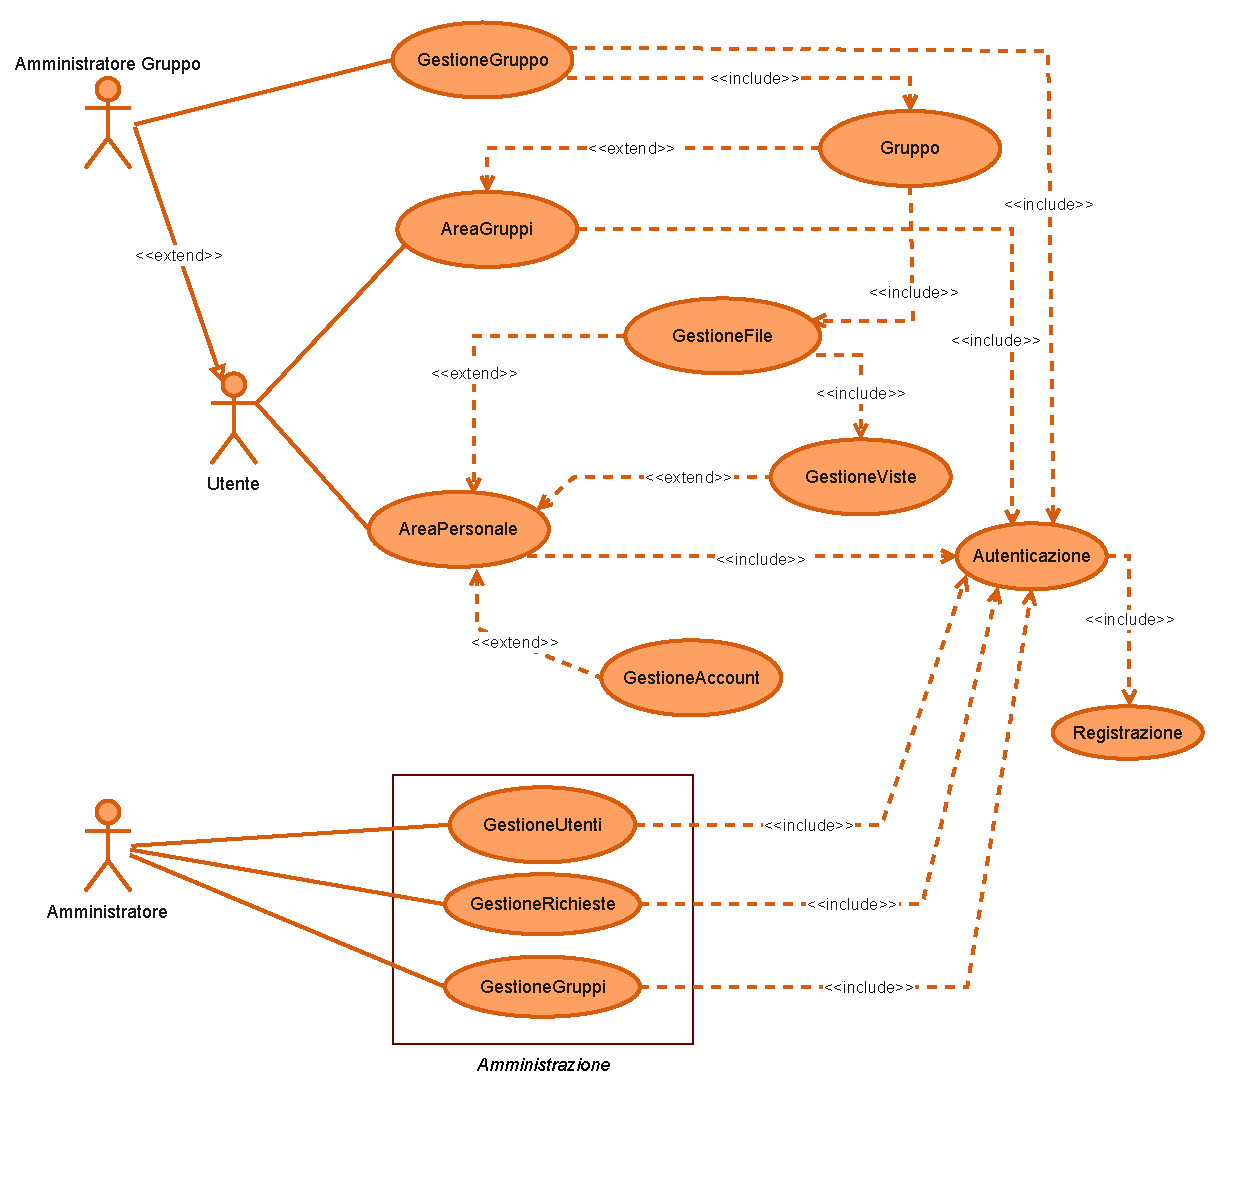
\includegraphics[scale=0.9]{casi d'uso/Casi d'uso-Casi d'uso.drawio.pdf}
\end{adjustwidth}

\phantomsection
\section*{Scenari}
\addcontentsline{toc}{section}{Scenari}

\phantomsection
\addcontentsline{toc}{subsection}{Registrazione}
\rowcolors{2}{white!0!}{white!0!}
\begin{adjustwidth}{0cm}{0cm}

\resizebox{1\textwidth}{!}{
\begin{tabular}{ |l|l|  }
\hline
\rowcolor{red!25}\large\textbf{Titolo} & \large{Registrazione}\\
\hline

\textbf{Descrizione} & L'utente si registra al servizio di Storage\\
\hline
\textbf{Attori} & Utente\\
\hline
\textbf{Relazioni} & \\
\hline
\textbf{Precondizioni} & L'utente non è registrato\\
\hline
\textbf{Postcondizioni} & \begin{tabular}{@{}l@{}} L'utente viene registrato nel sistema e gli viene allocato lo spazio di \\ archiviazione predefinito. Necessaria approvazione da parte dell'amministratore\end{tabular} \\
\hline
\textbf{Scenario principale} &
\begin{tabular}{@{}l@{}}
1) Si presenta all' utente una interfaccia per la registrazione dell' account\\  
2) L'utente inserisce le credenziali per la creazione dell' account\\
3) Il sistema controlla che l'utente non sia già registrato\\
4) La richiesta deve essere approvata dall'Amministratore
\end{tabular} \\
\hline
\textbf{Scenari alternativi} &
\begin{tabular}{@{}l@{}}
Scenario A: L'utente è già registrato \\
\quad 1) L'utente viene notificato dal servizio dell' errore\\
\quad 2) L'utente cambia username e riprova la registrazione\\
Scenario B: L'amministratore rifiuta la richiesta \\
\quad 1) L'utente non può accedere al servizio\\
\end{tabular} \\
\hline
\textbf{Requisiti non funzionali} & Interfaccia utente intuitiva\\
\hline
\textbf{Punti aperti} & \\
\hline

\end{tabular}
}
\end{adjustwidth}
\vspace{0.2cm}


\phantomsection
\addcontentsline{toc}{subsection}{Autenticazione}
\rowcolors{2}{white!0!}{white!0!}
\begin{adjustwidth}{0cm}{0cm}

\resizebox{1\textwidth}{!}{
\begin{tabular}{ |l|l|  }
\hline
\rowcolor{red!25}\large\textbf{Titolo} & \large{Autenticazione}\\
\hline

\textbf{Descrizione} & L'Utente effettua il login nel sistema\\
\hline
\textbf{Attori} & Utente, Amministratore, Amministratore di gruppo\\
\hline
\textbf{Relazioni} &\begin{tabular}{@{}l@{}} AreaPersonale, AreaGruppi, GestioneUtenti,\\ GestioneRichieste, GestioneGruppo\end{tabular} \\ 
\hline
\textbf{Precondizioni} & \begin{tabular}{@{}l@{}} L'Utente / Amministratore deve essere registrato nel sistema\end{tabular} \\
\hline
\textbf{Postcondizioni} & \\
\hline
\textbf{Scenario principale} &
\begin{tabular}{@{}l@{}}
1) Si presenta all'Utente / Amministratore un'interfaccia \\per l'autenticazione dell'account\\
2) L'Utente / Amministratore fornisce le credenziali \\
3) Il sistema effettua le opportune verifiche e, in caso di \\ approvazione, presenta la maschera dell'area pesonale
\end{tabular} \\
\hline
\textbf{Scenari alternativi} & 
\begin{tabular}{@{}l@{}}
Scenario A: Credenziali errate\\
\quad - Viene presentata nuovamente la maschera di Login
\end{tabular}\\
\hline
\textbf{Requisiti non funzionali} & Interfaccia utente intuitiva \\
\hline
\textbf{Punti aperti} & \\
\hline

\end{tabular}
}
\end{adjustwidth}
\vspace{0.2cm}


\phantomsection
\addcontentsline{toc}{subsection}{GestioneUtenti}
\rowcolors{2}{white!0!}{white!0!}
\begin{adjustwidth}{0cm}{0cm}

\resizebox{1\textwidth}{!}{
\begin{tabular}{ |l|l|  }
\hline
\rowcolor{red!25}\large\textbf{Titolo} & \large{GestioneUtenti}\\
\hline

\textbf{Descrizione} & Sezione per gestire gli utenti registrati\\
\hline
\textbf{Attori} & Amministratore\\
\hline
\textbf{Relazioni} & Autenticazione, GestioneAccount\\
\hline
\textbf{Precondizioni} &\\
\hline
\textbf{Postcondizioni} & \\
\hline
\textbf{Scenario principale} & \begin{tabular}{@{}l@{}} 
1) L'amministratore si autentica usando l'apposita pagina\\
2) L'amministratore si sposta sulla sezione dedicata alla moderazione degli utenti\\
3) Il sistema mostra la lista degli utenti registrati\\
4) L'amministratore può decidere effettuare le seguenti operazioni:\\
\quad - Eliminare un utente\\
\end{tabular}\\
\hline
\textbf{Scenari alternativi} & \\
\hline
\textbf{Requisiti non funzionali} & Pannello di amministrazione intuitivo\\
\hline
\textbf{Punti aperti} & \begin{tabular}{@{}l@{}} 
Altre operazioni eseguibili dall'amministratore:\\
\quad - Modificare la quantità di memoria disponibile per l'utente\\
\end{tabular}\\
\hline

\end{tabular}
}
\end{adjustwidth}
\vspace{0.5 cm}





\phantomsection
\addcontentsline{toc}{subsection}{GestioneRichieste}
\rowcolors{2}{white!0!}{white!0!}
\begin{adjustwidth}{0cm}{0cm}

\resizebox{1\textwidth}{!}{
\begin{tabular}{ |l|l|  }
\hline
\rowcolor{red!25}\large\textbf{Titolo} & \large{GestioneRichieste}\\
\hline

\textbf{Descrizione} & Gestisce le richieste degli utenti e dei gruppi\\
\hline
\textbf{Attori} & Amministratore\\
\hline
\textbf{Relazioni} & Autenticazione\\
\hline
\textbf{Precondizioni} &\\
\hline
\textbf{Postcondizioni} &\begin{tabular}{@{}l@{}} \end{tabular} \\
\hline
\textbf{Scenario principale} & \begin{tabular}{@{}l@{}} 
1) L'amministratore si autentica usando l'apposita pagina\\
2) L'amministratore si sposta sulla sezione dedicata alla moderazione\\
3) L'amministratore viene notificato delle richieste degli utenti e dei gruppi\\
4) L'amministratore può decidere effettuare le seguenti operazioni:\\
\quad - Accettare le richieste\\
\quad - Rifiutare le richieste\\
5) L'utente o il gruppo riceverà la risposta in base alla scelta dell'amministratore\\
\end{tabular}\\
\hline
\textbf{Scenari alternativi} & \\
\hline
\textbf{Requisiti non funzionali} & Pannello di amministrazione intuitivo\\
\hline
\textbf{Punti aperti} & L'amministratore non può gestire la richiesta al momento, si introduce lo stato "pendente"\\
\hline

\end{tabular}
}
\end{adjustwidth}
\vspace{0.2cm}





\phantomsection
\addcontentsline{toc}{subsection}{GestioneGruppi}
\rowcolors{2}{white!0!}{white!0!}
\begin{adjustwidth}{0cm}{0cm}
\resizebox{1\textwidth}{!}{
\begin{tabular}{ |l|l|  }
\hline
\rowcolor{red!25}\large\textbf{Titolo} & \large{GestioneGruppi}\\
\hline
\textbf{Descrizione} & Sezione per gestire i gruppi degli utenti registrati\\
\hline
\textbf{Attori} & Amministratore\\
\hline
\textbf{Relazioni} & Autenticazione\\
\hline
\textbf{Precondizioni} &\\
\hline
\textbf{Postcondizioni} & \\
\hline
\textbf{Scenario principale} & \begin{tabular}{@{}l@{}} 
1) L'amministratore si autentica usando l'apposita pagina\\
2) L'amministratore si sposta sulla sezione dedicata alla moderazione dei gruppi\\
3) Il sistema mostra la lista dei gruppi registrati\\
4) L'amministratore può decidere effettuare le seguenti operazioni:\\
\quad - Eliminare un gruppo\\
\end{tabular}\\
\hline
\textbf{Scenari alternativi} & \\
\hline
\textbf{Requisiti non funzionali} & Pannello di amministrazione intuitivo\\
\hline
\textbf{Punti aperti} & \begin{tabular}{@{}l@{}} 
Altre operazioni eseguibili dall'amministratore:\\
\quad - Modificare la quantità di memoria disponibile per il gruppo\\
\end{tabular}\\
\hline

\end{tabular}
}
\end{adjustwidth}
\vspace{0.2cm}



\phantomsection
\addcontentsline{toc}{subsection}{AreaPersonale}
\rowcolors{2}{white!0!}{white!0!}
\begin{adjustwidth}{0cm}{0cm}

\resizebox{1\textwidth}{!}{
\begin{tabular}{ |l|l|  }
\hline
\rowcolor{red!25}\large\textbf{Titolo} & \large{AreaPersonale}\\
\hline

\textbf{Descrizione} & Area Personale dell'utente\\
\hline
\textbf{Attori} & Utente\\
\hline
\textbf{Relazioni} & Autenticazione, GestioneAccount, GestioneViste, GestioneFile\\
\hline
\textbf{Precondizioni} &\\
\hline
\textbf{Postcondizioni} & \\
\hline
\textbf{Scenario principale} & 
\begin{tabular}{@{}l@{}} 
1) L'utente si autentica\\
2) All'utente viene presentata la pagina dell'area personale.\\
3) L'utente potrà spostarsi su tre diverse sezioni:\\
\quad - Gestione Account\\
\quad - Gestione File personali\\
\quad - Gestione Viste\\
\end{tabular}\\
\hline
\textbf{Scenari alternativi} & \\
\hline
\textbf{Requisiti non funzionali} & Interfaccia utente intuitiva\\
\hline
\textbf{Punti aperti} & \\
\hline

\end{tabular}
}
\end{adjustwidth}
\vspace{0.2cm}





\phantomsection
\addcontentsline{toc}{subsection}{GestioneAccount}
\rowcolors{2}{white!0!}{white!0!}
\begin{adjustwidth}{0cm}{0cm}

\resizebox{1\textwidth}{!}{
\begin{tabular}{ |l|l|  }
\hline
\rowcolor{red!25}\large\textbf{Titolo} & \large{GestioneAccount}\\
\hline

\textbf{Descrizione} & Gestione dell'account personale dell'utente\\
\hline
\textbf{Attori} & Utente\\
\hline
\textbf{Relazioni} & AreaPersonale\\
\hline
\textbf{Precondizioni} & L'utente si è autenticato\\
\hline
\textbf{Postcondizioni} & \\
\hline
\textbf{Scenario principale} & \begin{tabular}{@{}l@{}}
1) L'utente si sposta sulla sezione dedicata alla gestione dell'account personale\\
2) L'utente ha a disposizione le seguenti operazioni:\\
\quad - Modifica nickname\\
\quad - Modifica password\\
\quad - Eliminazione dell'account\\
\end{tabular}\\
\hline
\textbf{Scenari alternativi} & \\
\hline
\textbf{Requisiti non funzionali} & \\
\hline
\textbf{Punti aperti} & L'utente può modificare l'username\\
\hline

\end{tabular}
}
\end{adjustwidth}
\vspace{0.2cm}



\phantomsection
\addcontentsline{toc}{subsection}{GestioneViste}
\rowcolors{2}{white!0!}{white!0!}
\begin{adjustwidth}{0cm}{0cm}

\resizebox{1\textwidth}{!}{
\begin{tabular}{ |l|l|  }
\hline
\rowcolor{red!25}\large\textbf{Titolo} & \large{GestioneViste}\\
\hline

\textbf{Descrizione} & Sezione in cui l'utente modifica le viste\\
\hline
\textbf{Attori} & Utente\\
\hline
\textbf{Relazioni} & AreaPersonale, GestioneFile\\
\hline
\textbf{Precondizioni} & L'utente si è autenticato\\
\hline
\textbf{Postcondizioni} &\\
\hline
\textbf{Scenario principale} &
\begin{tabular}{@{}l@{}} 
1) L'utente si sposta sulla sezione dedicata alle viste\\
2) Il sistema presenta all'utente la lista di viste salvate ed un editor di viste\\
3) L'utente può:\\
\quad - Creare una nuova vista\\
\quad - Modificare una vista\\
\quad - Eliminare una vista\\
\end{tabular}\\
\hline
\textbf{Scenari alternativi} &
\begin{tabular}{@{}l@{}} 
Scenario A: Raggiunto il limite massimo di viste\\
\quad - È possibile modificare ed eliminare le viste, ma non crearne di nuove\\
\end{tabular}\\
\hline
\textbf{Requisiti non funzionali} & \\
\hline
\textbf{Punti aperti} & Editor grafico delle viste\\
\hline

\end{tabular}
}
\end{adjustwidth}
\vspace{0.2cm}





\phantomsection
\addcontentsline{toc}{subsection}{GestioneFile}
\rowcolors{2}{white!0!}{white!0!}
\begin{adjustwidth}{0cm}{0cm}

\resizebox{1\textwidth}{!}{
\begin{tabular}{ |l|l|  }
\hline
\rowcolor{red!25}\large\textbf{Titolo} & \large{GestioneFile}\\
\hline

\textbf{Descrizione} & Sezione in cui l'utente allo spazio di archiviazione personale\\
\hline
\textbf{Attori} & Utente\\
\hline
\textbf{Relazioni} & AreaPersonale, GestioneViste, AreaGruppi, GestioneGruppo\\
\hline
\textbf{Precondizioni} & L'utente si è autenticato\\
\hline
\textbf{Postcondizioni} &\\
\hline
\textbf{Scenario principale} &
\begin{tabular}{@{}l@{}} 
1) L'utente si sposta sulla sezione dedicata allo storage\\
2) Il sistema presenta all'utente il file manager dei file personali archiviati \\nel sistema\\
3) L'utente può:\\
\quad - Visualizzare i file/cartelle che ha caricato\\
\quad - Caricare uno o più file/cartelle\\
\quad - Scaricare un file/cartella\\
\quad - Eliminare file/cartelle\\
\quad - Modificare la visualizzazione dei file selezionando la vista opportuna\\
\end{tabular}\\
\hline
\textbf{Scenari alternativi} &
\begin{tabular}{@{}l@{}} 
Scenario A: Raggiunto il limite massimo di memoria di archiviazione\\
\quad - Non è possibile caricare nuovi file/cartelle\\
\end{tabular}\\
\hline
\textbf{Requisiti non funzionali} & 
\begin{tabular}{@{}l@{}} 
- Velocità nel caricare/scaricare file\\
- Organizzazione del file manager ampiamente personalizzabile\\
- Possibilità di cambiare le view in modo rapido\\
- Utilizzo efficace del servizio anche in assenza di una connessione veloce\\
\end{tabular}\\
\hline
\textbf{Punti aperti} & Anteprima file\\
\hline

\end{tabular}
}
\end{adjustwidth}
\vspace{0.2cm}



\phantomsection
\addcontentsline{toc}{subsection}{AreaGruppi}
\rowcolors{2}{white!0!}{white!0!}
\begin{adjustwidth}{0cm}{0cm}

\resizebox{1\textwidth}{!}{
\begin{tabular}{ |l|l|  }
\hline
\rowcolor{red!25}\large\textbf{Titolo} & \large{AreaGruppi}\\
\hline

\textbf{Descrizione} & Sezione dedicata ai gruppi di più utenti\\
\hline
\textbf{Attori} & Utente\\
\hline
\textbf{Relazioni} & Autenticazione, Gruppo\\
\hline
\textbf{Precondizioni} & L'utente si è autenticato\\
\hline
\textbf{Postcondizioni} & \\
\hline
\textbf{Scenario principale} &
\begin{tabular}{@{}l@{}}
1) L'utente si sposta sulla sezione dedicata ai gruppi\\
2) Viene mostrata la lista dei gruppi registrati nel sistema\\
3) L'utente può:\\
\quad - Iscriversi ad un gruppo, necessaria password\\
\quad - Creare un gruppo, la richiesta deve essere approvata da un amministratore\\
\quad - Esplorare un gruppo\\
\end{tabular}\\
\hline
\textbf{Scenari alternativi} & \\
\hline
\textbf{Requisiti non funzionali} & \\
\hline
\textbf{Punti aperti} & \\
\hline

\end{tabular}
}
\end{adjustwidth}
\vspace{0.2cm}



\phantomsection
\addcontentsline{toc}{subsection}{Gruppo}
\rowcolors{2}{white!0!}{white!0!}
\begin{adjustwidth}{0cm}{0cm}

\resizebox{1\textwidth}{!}{
\begin{tabular}{ |l|l|  }
\hline
\rowcolor{red!25}\large\textbf{Titolo} & \large{Gruppo}\\
\hline

\textbf{Descrizione} & Pagina del gruppo\\
\hline
\textbf{Attori} & Utente, Amministratore Gruppo\\
\hline
\textbf{Relazioni} & AreaGruppi, GestioneGruppo, GestioneFile\\
\hline
\textbf{Precondizioni} & L'utente si è autenticato\\
\hline
\textbf{Postcondizioni} & \\
\hline
\textbf{Scenario principale} &
\begin{tabular}{@{}l@{}}
1) L'utente entra nella sezione dedicata ad un gruppo\\
2) L'utente può:\\
\quad - Visualizzare la lista degli utenti iscritti al gruppo\\
\quad - Eseguire operazioni sui file del gruppo\\
\quad - Uscire dal gruppo\\
\end{tabular}\\
\hline
\textbf{Scenari alternativi} & \\
\hline
\textbf{Requisiti non funzionali} & \\
\hline
\textbf{Punti aperti} & \\
\hline

\end{tabular}
}
\end{adjustwidth}
\vspace{0.2cm}




\phantomsection
\addcontentsline{toc}{subsection}{GestioneGruppo}
\rowcolors{2}{white!0!}{white!0!}
\begin{adjustwidth}{0cm}{0cm}

\resizebox{1\textwidth}{!}{
\begin{tabular}{ |l|l|  }
\hline
\rowcolor{red!25}\large\textbf{Titolo} & \large{GestioneGruppo}\\
\hline

\textbf{Descrizione} & Pagina di amministrazione del gruppo\\
\hline
\textbf{Attori} & Amministratore Gruppo\\
\hline
\textbf{Relazioni} & Gruppo, Autenticazione\\
\hline
\textbf{Precondizioni} & \\
\hline
\textbf{Postcondizioni} & \\
\hline
\textbf{Scenario principale} &
\begin{tabular}{@{}l@{}}
1) L'amministratore del gruppo si autentica\\
2) L'amministratore del gruppo accede alla sezione del gruppo\\ di cui è amministratore\\
2) L'amministratore del gruppo può:\\
\quad - Visualizzare la lista degli utenti iscritti al gruppo\\
\quad - Aggiungere un utente al gruppo\\
\quad - Rimuovere un utente dal gruppo\\
\end{tabular}\\
\hline
\textbf{Scenari alternativi} & \\
\hline
\textbf{Requisiti non funzionali} & \\
\hline
\textbf{Punti aperti} & \\
\hline

\end{tabular}
}
\end{adjustwidth}
\vspace{0.2cm}

\pagebreak

\phantomsection
\section*{Analisi del Rischio}
\addcontentsline{toc}{section}{Analisi del Rischio}

\phantomsection
\addcontentsline{toc}{subsection}{Valutazione dei beni}

\rowcolors{2}{white!0!}{orange!10!}

\begin{adjustwidth}{-1.5cm}{0cm}

\resizebox{1.3\textwidth}{!}{
\begin{tabular}{ |l|l|l|  }
\hline
\rowcolor{red!80!}\multicolumn{3}{|c|}{\huge\textbf{\textcolor{white}{Valutazione dei beni}}} \\
\hline
\rowcolor{red!70!}\Large\textbf{\textcolor{white}{Bene}} & \Large\textbf{\textcolor{white}{Valore}} & \Large\textbf{\textcolor{white}{Esposizione}}\\
\hline

\textbf{Sistema Informativo} &
\begin{tabular}{@{}l@{}}
Alto.\\ Supporto alla gestione\\
dei dati utilizzati in molte delle funzionalità offerte\\ dal sistema.
\end{tabular} &
\begin{tabular}{@{}l@{}}
Alta.\\
Perdita economica e costi di ripristino.\\ 
Perdita d’immagine se la notizia diventa di\\
pubblico dominio.
\end{tabular} \\

\textbf{\begin{tabular}{@{}l@{}}
Informazioni relative \\agli utenti.
\end{tabular}}  &
\begin{tabular}{@{}l@{}}
Medio-Alto.\\
Informazioni relative agli utenti del sistema,\\
anche le credenziali,le quali\\ potrebbero permettere l’accesso ai file personali e di gruppo
\end{tabular} &
\begin{tabular}{@{}l@{}}
Medio-Alta.\\
Perdita d'immagine del Software, possibile\\
perdita dei file personali e di gruppo
\end{tabular} \\

\textbf{\begin{tabular}{@{}l@{}}
Informazioni relative \\all' Amministratore
\end{tabular}} &
\begin{tabular}{@{}l@{}}
Molto Alto.\\ Ha completa gestione sugli utenti e sui gruppi
\end{tabular} &
\begin{tabular}{@{}l@{}}
Molto Alta.\\
Possibilità di compromettere l'intero sistema,\\
perdita dei dati e dei file.\\
Perdita d'immagine del Software 
\end{tabular} \\


\textbf{Informazioni contenute nei file} &
\begin{tabular}{@{}l@{}}
Alto.\\ Informazioni private di utenti e gruppi.
\end{tabular} &
\begin{tabular}{@{}l@{}}
Alta.\\
Perdita d'immagine del Software, possibile \\perdita dei file personali e di gruppo 
\end{tabular} \\

\hline
\end{tabular}
}

\end{adjustwidth}




\pagebreak
\phantomsection
\addcontentsline{toc}{subsection}{Analisi minacce e controlli}

\rowcolors{2}{white!0!}{orange!10!}

\begin{adjustwidth}{-2cm}{0cm}

\resizebox{1.3\textwidth}{!}{
\begin{tabular}{ |l|l|l|l|  }
\hline
\rowcolor{red!80!}\multicolumn{4}{|c|}{\huge\textbf{\textcolor{white}{Analisi minacce e controlli}}} \\
\hline
\rowcolor{red!70!}\Large\textbf{\textcolor{white}{Minaccia}} & \Large\textbf{\textcolor{white}{Probabilità}} & \Large\textbf{\textcolor{white}{Controllo}} &
\Large\textbf{\textcolor{white}{Fattibilità}} \\
\hline

\begin{tabular}{@{}l@{}}
Furto d'identità \\(utente).
\end{tabular} & 
\begin{tabular}{@{}l@{}}
Media.\\ Username e password scelti \\
dall'utente potrebbero essere utilizzati\\
in altre applicazioni vulnerabili.
\end{tabular} &
\begin{tabular}{@{}l@{}}
Dopo alcuni tentativi errati viene \\
bloccato l’accesso.\\
Log di ogni operazione e degli indirizzi IP.
\end{tabular} & 
\begin{tabular}{@{}l@{}}
Basso costo di implementazione.
\end{tabular} \\

\begin{tabular}{@{}l@{}}
Furto d'identità \\(Amministratore).
\end{tabular} & 
\begin{tabular}{@{}l@{}}
Bassa.\\
Username e password stabiliti\\
dall'Amministratore,\\ numero di accessi limitato.\\
\end{tabular} &
\begin{tabular}{@{}l@{}}
Dopo alcuni tentativi errati viene \\
bloccato l’accesso.\\
Log di ogni operazione e degli indirizzi IP.
\end{tabular} & 
\begin{tabular}{@{}l@{}}
Basso costo di implementazione, \\
prestare attenzione all'accesso\\
ai dispositivi autenticati.
\end{tabular} \\

\begin{tabular}{@{}l@{}}
Intercettazione delle comunicazioni.
\end{tabular} &
\begin{tabular}{@{}l@{}}
Media.\\
Il servizio è realizzato in rete interna.
\end{tabular} &
\begin{tabular}{@{}l@{}}
Utilizzo di un sistema crittografico per la\\
cifratura delle comunicazioni.
\end{tabular} &
\begin{tabular}{@{}l@{}}
Basso costo, utilizzo di crittografia\\
simmetrica o asimmetrica.
\end{tabular}\\

\begin{tabular}{@{}l@{}}
Deny of Service
\end{tabular} &
\begin{tabular}{@{}l@{}}
Bassa.\\
poca probabilità di un attacco\\
DoS interno.
\end{tabular} &
\begin{tabular}{@{}l@{}}
- Progettazione adeguata e numero di\\
  operazioni di rete limitato.\\
- Log delle richieste.
\end{tabular} &
\begin{tabular}{@{}l@{}}
Basso costo, gestione delle richieste\\
e della rete delegata all' Amministratore.
\end{tabular} 
\\

\begin{tabular}{@{}l@{}}
Furto o modifica dei file
\end{tabular} &
\begin{tabular}{@{}l@{}}
Bassa.\\
difficile accedere \\
al file system dall'esterno.
\end{tabular} &
\begin{tabular}{@{}l@{}}
- Cifratura dei file\\
- Backup periodico
\end{tabular} &
\begin{tabular}{@{}l@{}}
Medio-Alto.\\
Cifratura dei file\\
potrebbe essere onerosa per il sistema.\\
Il backup periodico richiede\\
ulteriore spazio di archiviazione.
\end{tabular} 
\\

\hline
\end{tabular}
}

\end{adjustwidth}



\phantomsection
\addcontentsline{toc}{subsection}{Analisi tecnologica della sicurezza}

\rowcolors{2}{white!0!}{orange!10!}

\begin{adjustwidth}{-1cm}{0cm}

\resizebox{1.1\textwidth}{!}{
\begin{tabular}{ |l|l|  }
\hline
\rowcolor{red!80!}\multicolumn{2}{|c|}{\huge\textbf{\textcolor{white}{Analisi tecnologica della sicurezza}}} \\
\hline
\rowcolor{red!70!}\Large\textbf{\textcolor{white}{Tecnologia}} & \Large\textbf{\textcolor{white}{Vulnerabilità}} \\
\hline


\begin{tabular}{@{}l@{}}
Autenticazione \\
Username/Password
\end{tabular} &
\begin{tabular}{@{}l@{}}
- Password banali\\
- Utente rivela username e password\\
  volontariamente o con attacchi di\\
  ingegneria sociale.\\
- Attacco bruteforce sulle credenziali.
\end{tabular} 
\\

\begin{tabular}{@{}l@{}}
Cifratura della comunicazione\\
dei dati e dei file
\end{tabular} &
\begin{tabular}{@{}l@{}}
Cifratura Simmetrica:\\
\quad - Tempo di vita della chiave. Più \\
\quad informazioni cifro con la stessa chiave \\
\quad più materiale offro per l’analisi del \\
\quad testo ad un attaccante \\
\quad - Lunghezza chiave\\
\quad - Memorizzazione chiave\\
\\
Cifratura Asimmetrica:\\
\quad - Memorizzazione chiave\\
\end{tabular} 
\\

\begin{tabular}{@{}l@{}}
Architettura Client/Server \\
\end{tabular} &
\begin{tabular}{@{}l@{}}
- Vari tipi di attacchi Deny of Service.\\
- Intercettazione delle comunicazioni: \\
attacco Man in The Middle, Sniffing.

\end{tabular} 
\\




\hline
\end{tabular}
}

\end{adjustwidth}



\phantomsection
\section*{Security Use Case e Misuse Case}
\addcontentsline{toc}{subsection}{Security Use Case e Misuse Case}
\begin{adjustwidth}{-2cm}{0cm}
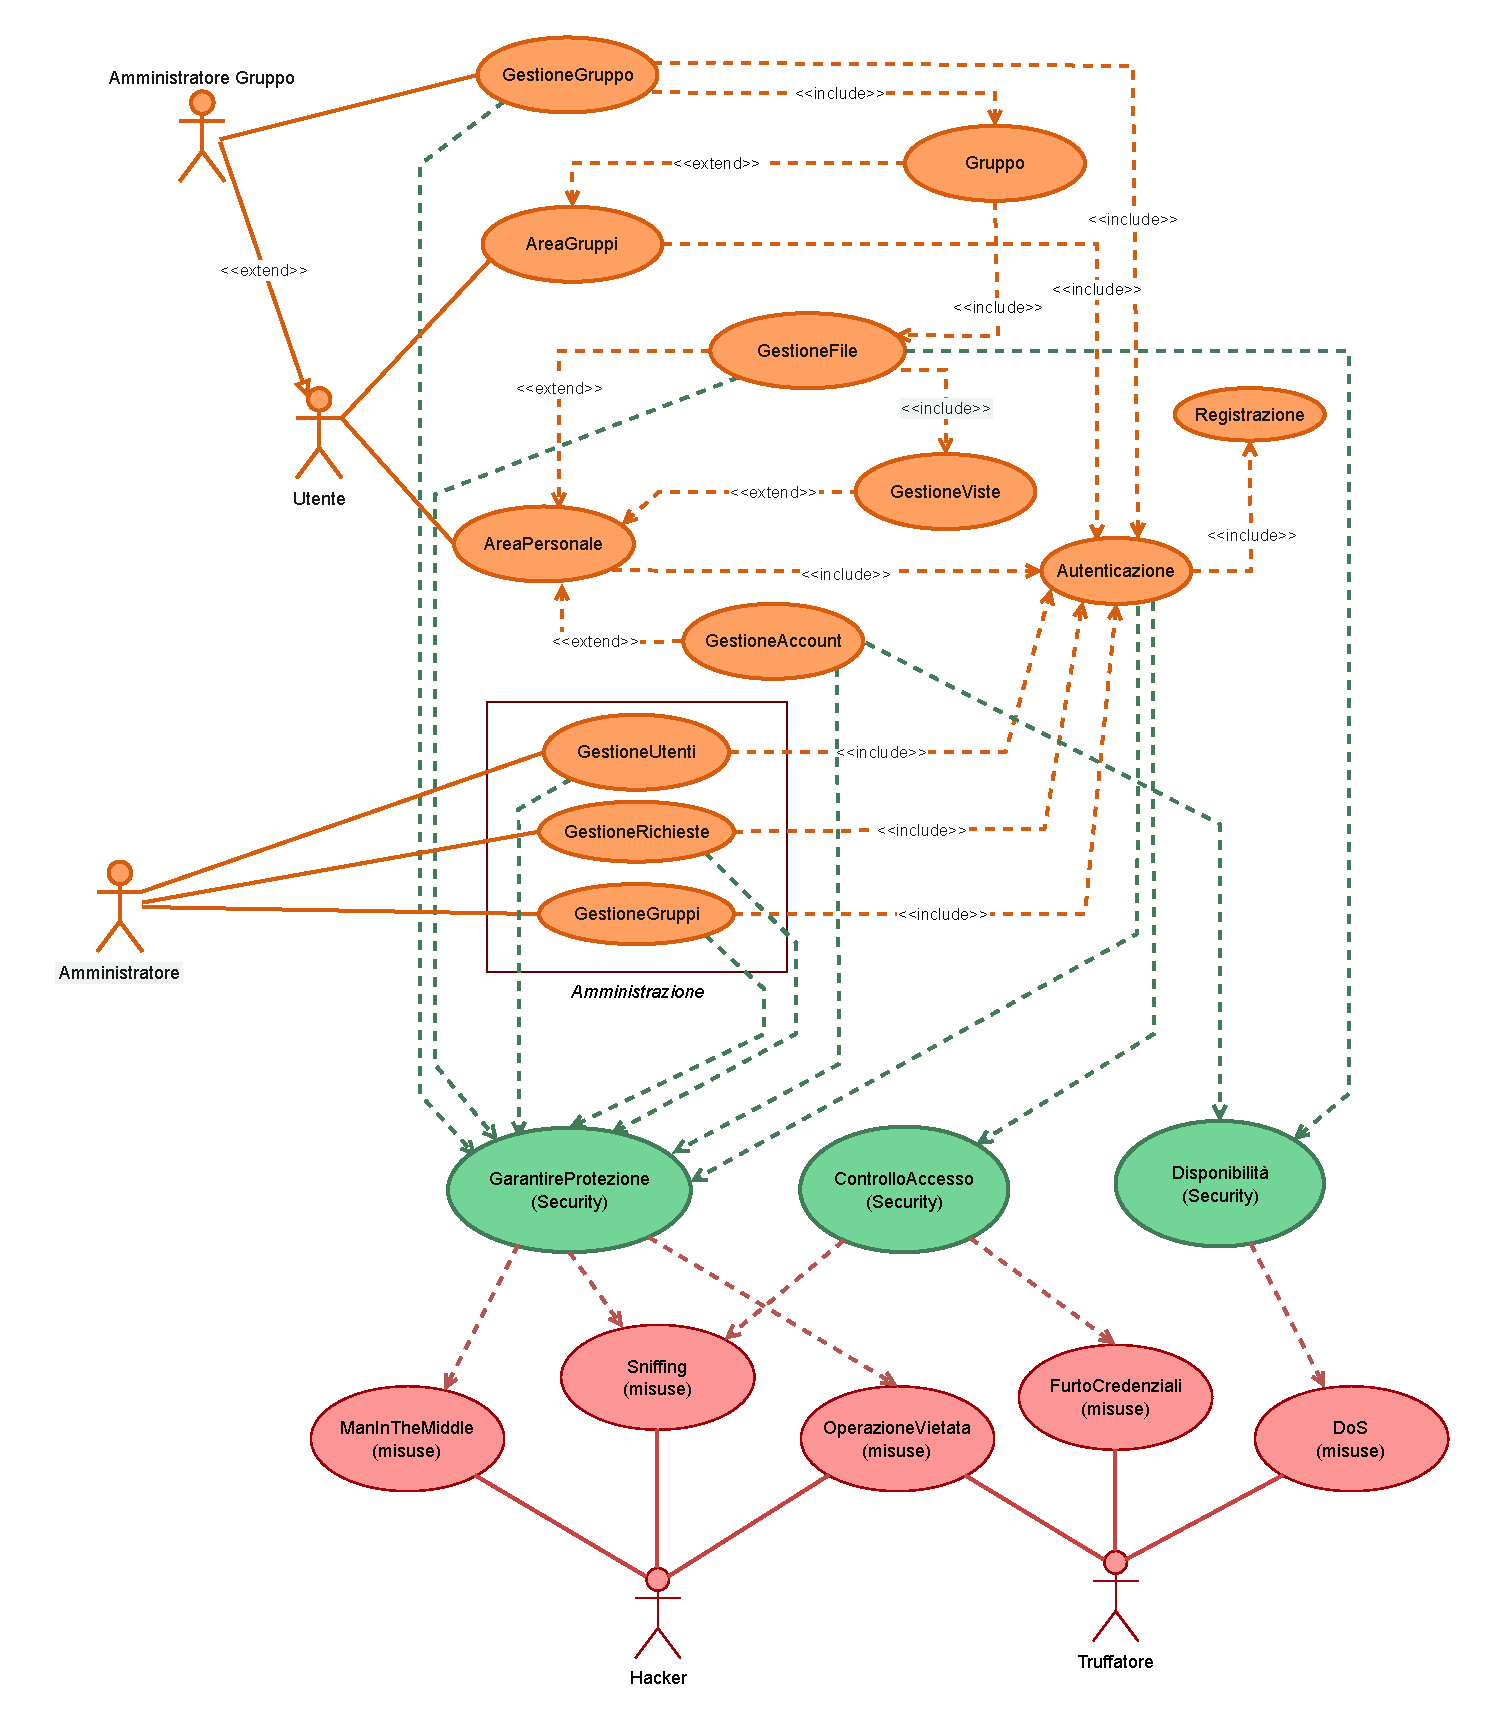
\includegraphics[scale=0.7]{casi d'uso/Casi d'uso-Casi d'uso e misuso.drawio.pdf}
\end{adjustwidth}




\phantomsection
\subsection*{Security Use Case e Misuse Case scenari}
\addcontentsline{toc}{subsection}{Security Use Case e Misuse Case scenari}

\rowcolors{2}{white!0!}{white!0!}


%------------------------------------

\phantomsection
\addcontentsline{toc}{subsubsection}{GarantireProtezione}

\begin{adjustwidth}{-1.5cm}{0cm}
\resizebox{1.2\textwidth}{!}{
\begin{tabular}{ |l|p{5cm}|p{5cm}|  }
\hline
\rowcolor{orange!45}\large\textbf{Titolo} & \multicolumn{2}{c|}{
 \large\textbf{GarantireProtezione}}\\
\hline

\textbf{Descrizione} & \multicolumn{2}{l|}{
Le comunicazioni e i file devono essere protetti }\\
\hline
\textbf{Misuse case} & \multicolumn{2}{l|}{
 ManInTheMiddle, Sniffing, OperazioneVietata }\\
\hline
\textbf{Precondizioni} &
\multicolumn{2}{p{10cm}|}{
L'attaccante o il truffatore ha i mezzi per attuare uno sniffing
delle comunicazioni, manomettere le operazioni tra il client e il server
o intaccare la cifratura dei file
}\\
\hline
\textbf{Postcondizioni} & \multicolumn{2}{l|}{
 Il sistema registra un tentativo di manomissione nei log}\\
\hline
& Sistema & Attaccante\\
\cline{2-3}
&
Cerca di garantire che i dati 
inviati all’Utente siano protetti, cifrati e
non possano essere modificati
& \\
\cline{2-3}
\multirow{-3 }{*}{\textbf{Scenario Principale}} & &
- Cerca di intercettare e manomettere le comunicazioni

- Cerca di estrarre dati o penetrare nel sistema in modo non autorizzato
\\

\hline
& Sistema & Attaccante\\
\cline{2-3}
&
- Garantisce che i dati sensibili ed i file salvati siano cifrati in maniera robusta

- Cerca di garantire la sicurezza da vulnerabilità
& 

\\
\cline{2-3}
\multirow{-3 }{*}{\textbf{Scenari di attacco avvenuto con successo}}
& 
&
- Cerca di aggirare la cifratura per ottenere le informazioni sensibili o i file

- Cerca e trova delle vulnerabilità per superare le difese del sistema
\\
\hline

\end{tabular}}
\end{adjustwidth}
\pagebreak


%------------------------------------

\phantomsection
\addcontentsline{toc}{subsubsection}{ControlloAccesso}

\begin{adjustwidth}{-1.5cm}{0cm}
\resizebox{1.2\textwidth}{!}{
\begin{tabular}{ |l|p{5cm}|p{5cm}|  }
\hline
\rowcolor{orange!45}\large\textbf{Titolo} & \multicolumn{2}{c|}{
 \large\textbf{ControlloAccesso}}\\
\hline

\textbf{Descrizione} & \multicolumn{2}{l|}{
L'accesso al servizio deve essere granulare e monitorato
 }\\
\hline
\textbf{Misuse case} & \multicolumn{2}{l|}{
 FurtoCredenziali, Sniffing }\\
\hline
\textbf{Precondizioni} &
\multicolumn{2}{p{10cm}|}{
L'attaccante dispone di un sistema per attuare un attacco a dizionario
}\\
\hline
\textbf{Postcondizioni} & \multicolumn{2}{l|}{
 Il sistema registra i tentativi ed avverte l'Amministratore
 }\\
\hline


& Sistema & Attaccante\\
\cline{2-3}
&
&
Cerca di individuare ed inserire
più volte le Credenziali di un
altro Utente/Amministratore
\\
\cline{2-3}
& 
L'accesso viene negato perché le Credenziali sono errate. Il tentativo di accesso viene registrato in un file di log.
&
\\
\cline{2-3}
\multirow{-4}{*}{\textbf{Scenario Principale}}
& 
Dopo 5 tentativi di accesso errati consecutivi viene bloccato l'accesso
&
\\
\hline



& Sistema & Attaccante\\
\cline{2-3}
&
& 
Accede al sistema
\\
\cline{2-3}
&
Concede l'accesso all'account e ai gruppi a cui l'account è collegato
&
\\
\cline{2-3}
&
&
Cerca di scaricare tutte le informazioni e di enumerare gli utenti
\\
\cline{2-3}
\multirow{-7}{*}{\textbf{Scenari di attacco avvenuto con successo}} 
&
Registra l'accesso nei log
& 
\\
\hline

\end{tabular}}
\end{adjustwidth}
\vspace{0.2cm}




%------------------------------------

\phantomsection
\addcontentsline{toc}{subsubsection}{Disponibilità}

\begin{adjustwidth}{-1.5cm}{0cm}
\resizebox{1.2\textwidth}{!}{
\begin{tabular}{ |l|p{5cm}|p{5cm}|  }
\hline
\rowcolor{orange!45}\large\textbf{Titolo} & \multicolumn{2}{c|}{
 \large\textbf{Disponibilità}}\\
\hline

\textbf{Descrizione} & \multicolumn{2}{l|}{
Il sistema deve sempre fornire servizio
 }\\
\hline
\textbf{Misuse case} & \multicolumn{2}{l|}{
 DoS}\\
\hline
\textbf{Precondizioni} & 
\multicolumn{2}{p{10cm}|}{
L'attaccante dispone di un ambiente per effettuare un attacco efficace
}\\
\hline
\textbf{Postcondizioni} & \multicolumn{2}{p{10cm}|}{
Il sistema monitora il flusso di dati ed eventualmente attua politiche di protezione o ripristino
 }\\
 
\hline

& Sistema & Attaccante\\
\cline{2-3}
&
&
Avvia l'attacco 
\\
\cline{2-3}
\multirow{-2}{*}{\textbf{Scenario Principale}}
&
Registra l'attacco nei log ed eventualmente esegue un ripristino
&
\\
\hline



& Sistema & Attaccante\\
\cline{2-3}
&
&
Riesce a creare un grande flusso di dati
\\
\cline{2-3}
&
Non riesce a contenere l'attacco 
&
\\
\cline{2-3}
&
Non è possibile il ripristino immediato del sistema
&
\\
\cline{2-3}
\multirow{-7}{*}{\textbf{Scenari di attacco avvenuto con successo}} 
&
& 
Riesce a creare un disservizio
\\
\hline



\end{tabular}}
\end{adjustwidth}
\pagebreak




%--------------------------------------------------------

\phantomsection
\addcontentsline{toc}{subsection}{Requisiti Funzionali aggiornati}

\rowcolors{2}{green!0!}{orange!10!}

\begin{adjustwidth}{1cm}{0cm}

\resizebox{0.9\textwidth}{!}{
\begin{tabular}{ |c|p{11cm}|  }
\hline
\rowcolor{blue!55}\multicolumn{2}{|c|}{\Large\textbf{Requisiti Funzionali aggiornati}} \\
\hline
\rowcolor{blue!45}\LARGE{ID} & \LARGE{Requisito}\\
\hline

\textbf{R12F} & Produzione di file di log per tenere traccia delle operazioni\\
\textbf{R13F} & L'Amministratore può accedere al file di log per controllare e gestire eventuali segnalazione da parte del sistema\\
\textbf{R14F} & Il sistema è protetto da una ACL\\
\textbf{R15F} & Il sistema deve essere in grado di ripristinarsi in seguito ad un attacco DoS\\

\hline
\end{tabular}
}

\end{adjustwidth}
\vspace{1cm}




\phantomsection
\addcontentsline{toc}{subsection}{Requisiti Non Funzionali aggiornati}

\rowcolors{2}{green!0!}{orange!10!}

\begin{adjustwidth}{1cm}{0cm}

\resizebox{0.9\textwidth}{!}{
\begin{tabular}{ |c|p{11cm}|  }
\hline
\rowcolor{purple!55}\multicolumn{2}{|c|}{\Large\textbf{Requisiti Non Funzionali aggiornati}} \\
\hline
\rowcolor{purple!45}\LARGE{ID} & \LARGE{Requisito}\\
\hline

\textbf{R7NF} & Il sistema deve essere in grado di effettuare un ripristino veloce in caso di attacco\\

\textbf{R8NF} & Backup periodico dei dati\\
\hline
\end{tabular}
}

\end{adjustwidth}
\vspace{1cm}

%-----------------------------------------------
\phantomsection
\addcontentsline{toc}{subsection}{Vocabolario aggiornato}

\rowcolors{2}{green!0!}{orange!10!}

\begin{adjustwidth}{1cm}{0cm}

\resizebox{0.9\textwidth}{!}{
\Large
\begin{tabular}{ |c|p{8cm}|c|  }
\hline
\rowcolor{red!60}\multicolumn{3}{|c|}{\Large\textbf{Vocabolario aggiornato}} \\
\hline
\rowcolor{red!50}\LARGE{Voce} & \LARGE{Definizione} & \LARGE{Sinonimo}\\
\hline

\textbf{Log} & File in cui vengono registrate le informazioni di Sistema e di Sicurezza & File di log \\

\textbf{ACL} & Sistema che monitora gli accessi & \\
 
\hline
\end{tabular}
}

\end{adjustwidth}
\vspace{1cm}

%-------------------------------------------

\phantomsection
\section*{Casi d'uso aggiornati}
\addcontentsline{toc}{subsection}{Casi d'uso aggiornati}
\begin{adjustwidth}{-2cm}{0cm}
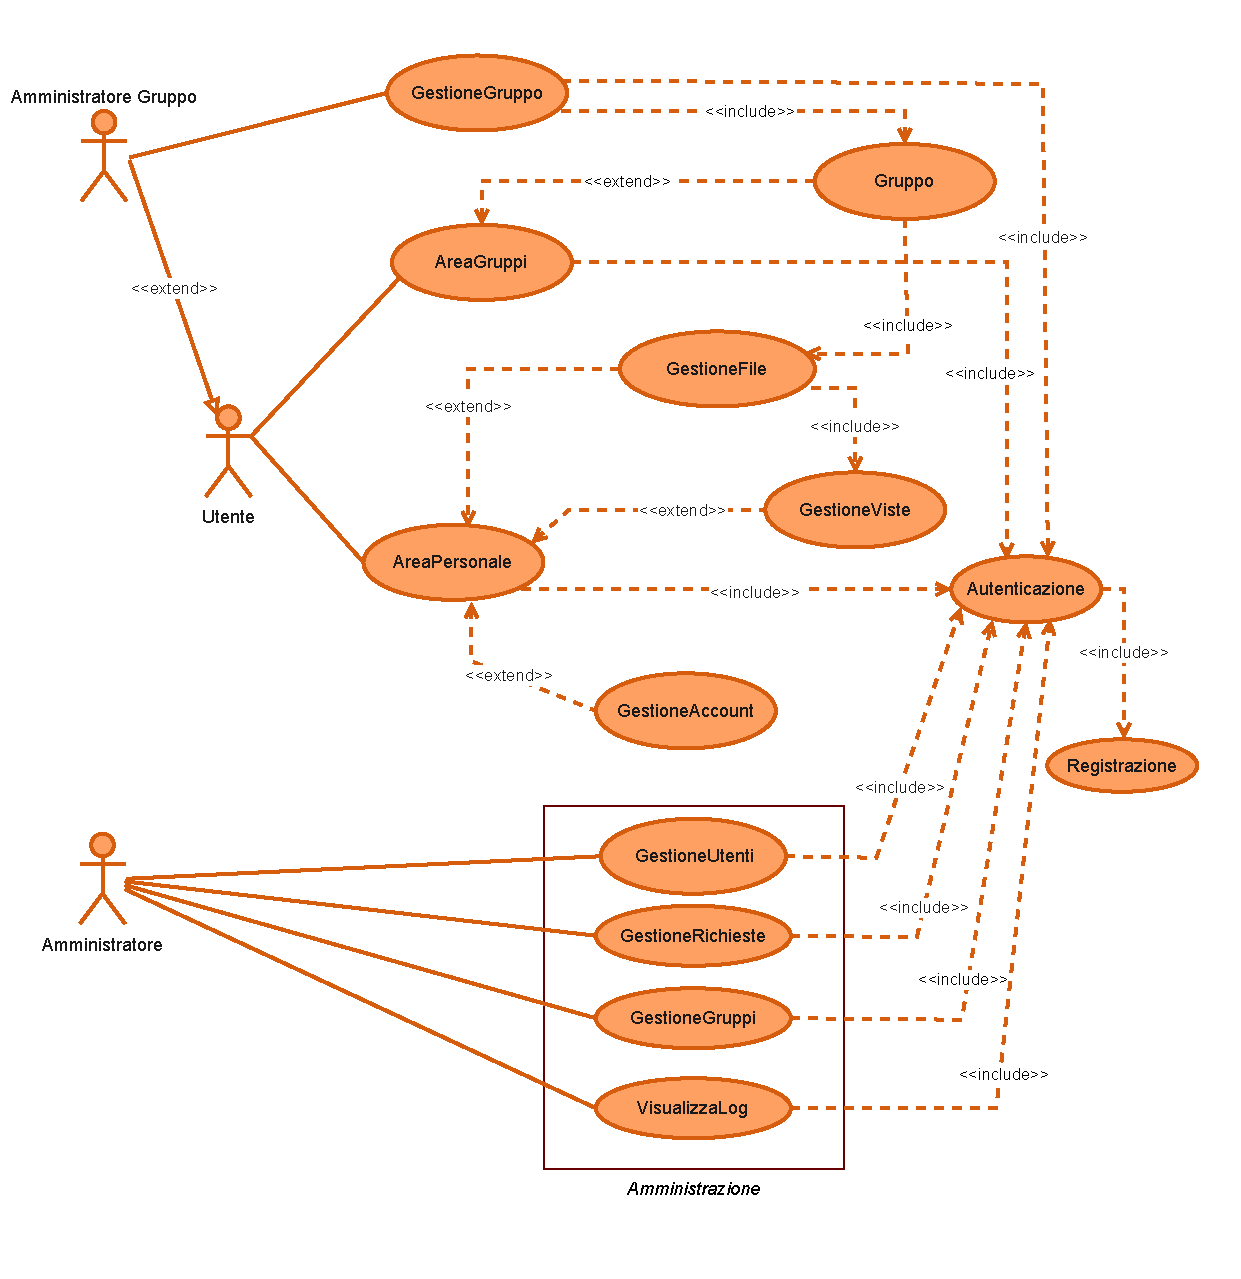
\includegraphics[scale=0.9]{casi d'uso/Casi d'uso-Casi d'uso aggiornati.drawio.pdf}
\end{adjustwidth}



\phantomsection
\addcontentsline{toc}{subsection}{VisualizzaLog}
\rowcolors{2}{white!0!}{white!0!}
\begin{adjustwidth}{0cm}{0cm}

\resizebox{1\textwidth}{!}{
\begin{tabular}{ |l|l|  }
\hline
\rowcolor{red!25}\large\textbf{Titolo} & \large{VisualizzaLog}\\
\hline

\textbf{Descrizione} & Pagina di monitoraggio dei Log\\
\hline
\textbf{Attori} & Amministratore Gruppo\\
\hline
\textbf{Relazioni} & Autenticazione\\
\hline
\textbf{Precondizioni} & \\
\hline
\textbf{Postcondizioni} & \\
\hline
\textbf{Scenario principale} &
\begin{tabular}{@{}l@{}}
1) Autenticazione\\
2) L'Amministratore accede alla sezione dei Log\\
2) L'Amministratore del gruppo può visualizzare\\
\quad i Log di sistema
\end{tabular}\\
\hline
\textbf{Scenari alternativi} & \\
\hline
\textbf{Requisiti non funzionali} & \\
\hline
\textbf{Punti aperti} & \\
\hline

\end{tabular}
}
\end{adjustwidth}
\vspace{0.2cm}
\pagebreak

\chapter*{Analisi del Problema}
\addcontentsline{toc}{chapter}{Analisi del Probelma}

\phantomsection
\section*{Analisi delle Funzionalità}
\addcontentsline{toc}{section}{Analisi delle Funzionalità}

\phantomsection
\addcontentsline{toc}{subsection}{Tabella delle Funzionalità}
\thispagestyle{empty}

\rowcolors{2}{white!0!}{white!0!}

\begin{adjustwidth}{-1cm}{0cm}

\resizebox{1.2\textwidth}{!}{
\begin{tabular}{ |c|p{4cm}|c|c|  }
\hline
\rowcolor{darktangerine!60}\multicolumn{4}{|c|}{\huge\textbf{Tabella delle Funzionalità}} \\
\hline
\rowcolor{darktangerine!50!}\LARGE\textbf{Funzionalità} & \multicolumn{1}{c|}{\LARGE\textbf{Tipo}} & 
\LARGE\textbf{Complessità} & \LARGE\textbf{Requisiti}\\
\hline
\hline
\rowcolor{cyan!10!}
\textbf{Registrazione} & Memorizzazione dati & Semplice & R1F \\ \hline
\rowcolor{cyan!10!}
\textbf{Autenticazione} & Interazione con l'esterno, Gestione dati & Semplice & R2F \\ \hline
\rowcolor{red!20!}
\textbf{GestioneUtenti} & Gestione dati, interazione con l’esterno & Semplice & R5F \\ \hline
\rowcolor{orange!20!}
\textbf{GestioneRichieste} & Gestione dati, interazione con l’esterno & Semplice &  R5F \\ \hline  
\rowcolor{yellow!20!}
\textbf{GestioneGruppi} & Gestione dati, interazione con l’esterno & Semplice & R5F \\ \hline  
\rowcolor{darktangerine!10!}
\textbf{VisualizzaLog} & Interazione con l’esterno & Semplice & R12F \\ \hline  
\rowcolor{yellow!20!}
\textbf{CreazioneBackup} & Memorizzazione dati & Semplice & R8NF \\ \hline
\rowcolor{blue!20!}
\textbf{AreaPersonale} & Memorizzazione dati, Gestione dati, interazione con l’esterno & Complesso & R3F, R9F\\ 
\rowcolor{cyan!30!} \hline
\textbf{GestioneAccount} & Memorizzazione dati, Gestione dati, interazione con l’esterno & Complesso & R10F \\
\rowcolor{cyan!20!}
\textbf{CambioCredenziali} & Memorizzazione dati, Gestione dati, interazione con l’esterno & Semplice & R10F \\
\rowcolor{cyan!20!}
\textbf{RimozioneAccount} & Gestione dati, interazione con l’esterno & Semplice & R10F \\ 
\rowcolor{cyan!20!}
\textbf{VisualizzaInformazioni} & Interazione con l’esterno & Semplice & R10F \\ \hline


\end{tabular}}
\end{adjustwidth}
\pagebreak


\begin{adjustwidth}{-1cm}{0cm}
\resizebox{1.2\textwidth}{!}{
\begin{tabular}{ |l|p{4cm}|l|l| }

\hline
\rowcolor{red!25!}
\textbf{GestioneViste} & Memorizzazione dati, Gestione dati, interazione con l’esterno & Complesso & R9F \\
\rowcolor{orange!20!}
\textbf{CreazioneVista} & Memorizzazione dati, interazione con l’esterno & Semplice & R9F \\
\rowcolor{orange!20!}
\textbf{RimozioneVista} & Gestione dati, interazione con l’esterno & Semplice & R9F \\
\rowcolor{orange!20!}
\textbf{PersonalizzaVista} & Memorizzazione dati, Gestione dati, interazione con l’esterno & Semplice & R9F \\\hline

\rowcolor{green!25!}
\textbf{GestioneFile} & Memorizzazione dati, gestione dati, interazione con l’esterno & Complesso & R3F, R4F \\ 
\rowcolor{lime!20!}
\textbf{CaricaFile} & Memorizzazione dati, interazione con l’esterno & Semplice & R3F, R4F \\ 
\rowcolor{lime!20!}
\textbf{ScaricaFile} & Gestione dati, interazione con l’esterno & Semplice & R3F, R4F \\ 
\rowcolor{lime!20!}
\textbf{EliminaFile} & Gestione dati, interazione con l’esterno & Semplice & R3F, R4F \\ 
\hline

\rowcolor{violet!20!}
\textbf{AreaGruppi} & Gestione dati, interazione con l’esterno & Complesso & R6F, R7F, R8F \\ 
\rowcolor{magenta!20!} \hline
\textbf{CreaGruppo} & Memorizzazione dati, interazione con l’esterno & Semplice & R6F, R7F, R8F \\
\rowcolor{magenta!20!} \hline
\textbf{IscrizioneGruppo} & Gestione dati, interazione con l’esterno & Semplice & R6F, R7F, R8F \\
\hline

\rowcolor{magenta!20!}
\textbf{EsploraGruppo} & Memorizzazione dati, Gestione dati, interazione con l’esterno & Complesso & R8F \\ 
\rowcolor{pink!30!}
\textbf{VisualizzaUtenti} & Interazione con l’esterno & Semplice & R6F, R7F, R8F \\
\rowcolor{pink!30!}
\textbf{GestioneFileGruppo} & Memorizzazione dati, Gestione dati, interazione con l’esterno & Semplice & R6F, R7F, R8F \\
\rowcolor{pink!30!}
\textbf{UscitaGruppo} & Gestione dati, interazione con l’esterno & Semplice & R6F, R7F, R8F \\
\hline

\rowcolor{magenta!20!}
\textbf{GestioneGruppo} & Memorizzazione dati, gestione dati, interazione con l’esterno & Complesso & R5F, R6F \\ 
\rowcolor{pink!30!}
\textbf{GestioneUtentiGruppo} & Gestione dati, interazione con l’esterno & Semplice & R6F, R7F, R8F \\
\hline

\end{tabular}
}

\end{adjustwidth}


%---------------------------------------------------------------------------------
\phantomsection
\subsection*{Tabelle di Informazione/Flusso}
\addcontentsline{toc}{subsection}{Tabelle di Informazione/Flusso}

\phantomsection
\addcontentsline{toc}{subsubsection}{Registrazione}

\rowcolors{2}{white!0!}{white!0!}
\begin{adjustwidth}{-2cm}{0cm}
\resizebox{1.3\textwidth}{!}{
\begin{tabular}{ |m{3cm}|c|m{2.7cm}|m{2.5cm}|m{2.5cm}|  }
\hline
\rowcolor{darkspringgreen!50}\multicolumn{5}{|c|}{\Large\textbf{Registrazione}} \\
\hline
\rowcolor{emerald!50}\Large\textbf{Informazione} & \Large\textbf{Tipo}& \Large\textbf{Livello   
protezione   /privacy} & \Large\textbf{Input /Output}& \Large\textbf{Vincoli}\\
\hline
Nickname & Semplice & Alto & Input &  Non più di 32 caratteri\\
\hline
Username & Semplice & Alto & Input &  Non più di 32 caratteri\\
\hline
Password & Semplice & Molto Alto & Input &  Non meno di 6 caratteri, non più di 128 caratteri\\
\hline
\end{tabular}
}
\end{adjustwidth}
\vspace{0.6cm}

%--------

\phantomsection
\addcontentsline{toc}{subsubsection}{Autenticazione}

\rowcolors{2}{white!0!}{white!0!}
\begin{adjustwidth}{-2cm}{0cm}
\resizebox{1.3\textwidth}{!}{
\begin{tabular}{ |m{3cm}|c|m{2.7cm}|m{2.5cm}|m{2.5cm}|  }
\hline
\rowcolor{darkspringgreen!50}\multicolumn{5}{|c|}{\Large\textbf{Autenticazione}} \\
\hline
\rowcolor{emerald!50}\Large\textbf{Informazione} & \Large\textbf{Tipo}& \Large\textbf{Livello   
protezione   /privacy} & \Large\textbf{Input /Output}& \Large\textbf{Vincoli}\\
\hline
Username & Semplice & Alto & Input &  Non più di 32 caratteri\\
\hline
Password & Semplice & Molto Alto & Input &  Non meno di 6 caratteri, non più di 128 caratteri\\
\hline
\end{tabular}
}
\end{adjustwidth}
\vspace{0.6cm}

%--------

\phantomsection
\addcontentsline{toc}{subsubsection}{GestioneUtenti}

\rowcolors{2}{white!0!}{white!0!}
\begin{adjustwidth}{-2cm}{0cm}
\resizebox{1.3\textwidth}{!}{
\begin{tabular}{ |m{3cm}|c|m{2.7cm}|m{2.5cm}|m{2.5cm}|  }
\hline
\rowcolor{darkspringgreen!50}\multicolumn{5}{|c|}{\Large\textbf{GestioneUtenti}} \\
\hline
\rowcolor{emerald!50}\Large\textbf{Informazione} & \Large\textbf{Tipo}& \Large\textbf{Livello   
protezione   /privacy} & \Large\textbf{Input /Output}& \Large\textbf{Vincoli}\\
\hline
Utente & Composto & Alto & Output &  \\
\hline
\textbf{Composto da:} & & & & \\
Nickname & Semplice & Basso & Output &  Non più di 32 caratteri\\
Username & Semplice & Medio & Output &  Non più di 32 caratteri\\
\hline
\end{tabular}
}
\end{adjustwidth}
\vspace{0.6cm}

%--------

\phantomsection
\addcontentsline{toc}{subsubsection}{GestioneRichieste}

\rowcolors{2}{white!0!}{white!0!}
\begin{adjustwidth}{-2cm}{0cm}
\resizebox{1.3\textwidth}{!}{
\begin{tabular}{ |m{3cm}|c|m{2.7cm}|m{2.5cm}|m{2.5cm}|  }
\hline
\rowcolor{darkspringgreen!50}\multicolumn{5}{|c|}{\Large\textbf{GestioneRichieste}} \\
\hline
\rowcolor{emerald!50}\Large\textbf{Informazione} & \Large\textbf{Tipo}& \Large\textbf{Livello   
protezione   /privacy} & \Large\textbf{Input /Output}& \Large\textbf{Vincoli}\\
\hline
RichiestaUtente & Composto & Alto & Output &  \\
\hline
\textbf{Composto da:} & & & & \\
Username & Semplice & Medio & Output &  Non più di 32 caratteri\\
Timestamp & Semplice & Basso & Output & Esattamente 23 caratteri\\
\hline

RichiestaGruppo & Composto & Medio & Output &  \\
\hline
\textbf{Composto da:} & & & & \\
NomeGruppo & Semplice & Basso & Output &  Non più di 32 caratteri\\
NomeProprietario & Semplice & Medio & Output &  Non più di 32 caratteri\\
Timestamp & Semplice & Basso & Output & Esattamente 23 caratteri\\
\hline
\end{tabular}
}
\end{adjustwidth}
\vspace{0.6cm}

%--------

\phantomsection
\addcontentsline{toc}{subsubsection}{GestioneGruppi}

\rowcolors{2}{white!0!}{white!0!}
\begin{adjustwidth}{-2cm}{0cm}
\resizebox{1.3\textwidth}{!}{
\begin{tabular}{ |m{3cm}|c|m{2.7cm}|m{2.5cm}|m{2.5cm}|  }
\hline
\rowcolor{darkspringgreen!50}\multicolumn{5}{|c|}{\Large\textbf{GestioneGruppi}} \\
\hline
\rowcolor{emerald!50}\Large\textbf{Informazione} & \Large\textbf{Tipo}& \Large\textbf{Livello   
protezione   /privacy} & \Large\textbf{Input /Output}& \Large\textbf{Vincoli}\\
\hline
Gruppo & Composto & Alto & Output &  \\
\hline
\textbf{Composto da:} & & & & \\
NomeGruppo & Semplice & Basso & Output &  Non più di 32 caratteri\\
Descrizione & Semplice & Basso & Output &  Non più di 256 caratteri\\
NumeroPartecipanti & Semplice & Medio & Output &  Non più di 16 partecipanti\\
\hline
\end{tabular}
}
\end{adjustwidth}
\vspace{0.6cm}

%--------


\phantomsection
\addcontentsline{toc}{subsubsection}{VisualizzaLog}

\rowcolors{2}{white!0!}{white!0!}
\begin{adjustwidth}{-2cm}{0cm}
\resizebox{1.3\textwidth}{!}{
\begin{tabular}{ |m{3cm}|c|m{2.7cm}|m{2.5cm}|m{2.5cm}|  }
\hline
\rowcolor{darkspringgreen!50}\multicolumn{5}{|c|}{\Large\textbf{VisualizzaLog}} \\
\hline
\rowcolor{emerald!50}\Large\textbf{Informazione} & \Large\textbf{Tipo}& \Large\textbf{Livello   
protezione   /privacy} & \Large\textbf{Input /Output}& \Large\textbf{Vincoli}\\
\hline
ResocontoLog & Composto & Alto & Output &  \\
\hline
\textbf{Composto da:} & & & & \\
Timestamp & Semplice & Basso & Output & Esattamente 23 caratteri\\
EventoLog & Semplice & Alto & Output &  Non più di 256 caratteri\\
\hline
\end{tabular}
}
\end{adjustwidth}
\vspace{0.6cm}


\phantomsection
\addcontentsline{toc}{subsubsection}{CambioCredenziali}

\rowcolors{2}{white!0!}{white!0!}
\begin{adjustwidth}{-2cm}{0cm}
\resizebox{1.3\textwidth}{!}{
\begin{tabular}{ |m{3cm}|c|m{2.7cm}|m{2.5cm}|m{2.5cm}|  }
\hline
\rowcolor{darkspringgreen!50}\multicolumn{5}{|c|}{\Large\textbf{CambioCredenziali}} \\
\hline
\rowcolor{emerald!50}\Large\textbf{Informazione} & \Large\textbf{Tipo}& \Large\textbf{Livello   
protezione   /privacy} & \Large\textbf{Input /Output}& \Large\textbf{Vincoli}\\
\hline
Nickname & Semplice & Alto & Output &  Non più di 32 caratteri\\
\hline
Username & Semplice & Alto & Output &  Non più di 32 caratteri\\
\hline
NuovoNickname & Semplice & Alto & Input &  Non più di 32 caratteri\\
\hline
NuovoUsername & Semplice & Alto & Input &  Non più di 32 caratteri\\
\hline
NuovaPassword & Semplice & Alto & Input &  Non meno di 6 caratteri, non più di 128 caratteri\\
\hline

\end{tabular}
}
\end{adjustwidth}
\vspace{0.6cm}



\phantomsection
\addcontentsline{toc}{subsubsection}{RimozioneAccount}

\rowcolors{2}{white!0!}{white!0!}
\begin{adjustwidth}{-2cm}{0cm}
\resizebox{1.3\textwidth}{!}{
\begin{tabular}{ |m{3cm}|c|m{2.7cm}|m{2.5cm}|m{2.5cm}|  }
\hline
\rowcolor{darkspringgreen!50}\multicolumn{5}{|c|}{\Large\textbf{RimozioneAccount}} \\
\hline
\rowcolor{emerald!50}\Large\textbf{Informazione} & \Large\textbf{Tipo}& \Large\textbf{Livello   
protezione   /privacy} & \Large\textbf{Input /Output}& \Large\textbf{Vincoli}\\
\hline
Password & Semplice & Molto Alto & Input &  Non meno di 6 caratteri, non più di 128 caratteri\\
\hline
\end{tabular}
}
\end{adjustwidth}
\vspace{0.6cm}


\phantomsection
\addcontentsline{toc}{subsubsection}{VisualizzaInformazioni}

\rowcolors{2}{white!0!}{white!0!}
\begin{adjustwidth}{-2cm}{0cm}
\resizebox{1.3\textwidth}{!}{
\begin{tabular}{ |m{3cm}|c|m{2.7cm}|m{2.5cm}|m{2.5cm}|  }
\hline
\rowcolor{darkspringgreen!50}\multicolumn{5}{|c|}{\Large\textbf{VisualizzaInformazioni}} \\
\hline
\rowcolor{emerald!50}\Large\textbf{Informazione} & \Large\textbf{Tipo}& \Large\textbf{Livello   
protezione   /privacy} & \Large\textbf{Input /Output}& \Large\textbf{Vincoli}\\
\hline
Nickname & Semplice & Basso & Output &  Non più di 32 caratteri\\
Username & Semplice & Basso & Output &  Non più di 32 caratteri\\
\hline
\end{tabular}
}
\end{adjustwidth}
\vspace{0.6cm}




\phantomsection
\addcontentsline{toc}{subsubsection}{CreazioneVista}

\rowcolors{2}{white!0!}{white!0!}
\begin{adjustwidth}{-2cm}{0cm}
\resizebox{1.3\textwidth}{!}{
\begin{tabular}{ |m{3cm}|c|m{2.7cm}|m{2.5cm}|m{2.5cm}|  }
\hline
\rowcolor{darkspringgreen!50}\multicolumn{5}{|c|}{\Large\textbf{CreazioneVista}} \\
\hline
\rowcolor{emerald!50}\Large\textbf{Informazione} & \Large\textbf{Tipo}& \Large\textbf{Livello   
protezione   /privacy} & \Large\textbf{Input /Output}& \Large\textbf{Vincoli}\\
\hline
NomeVista & Semplice & Basso & Input & Non più di 32 caratteri\\
StileVista & Semplice & Basso & Input & \\
\hline
\end{tabular}
}
\end{adjustwidth}
\vspace{0.6cm}

\phantomsection
\addcontentsline{toc}{subsubsection}{RimozioneVista}

\rowcolors{2}{white!0!}{white!0!}
\begin{adjustwidth}{-2cm}{0cm}
\resizebox{1.3\textwidth}{!}{
\begin{tabular}{ |m{3cm}|c|m{2.7cm}|m{2.5cm}|m{2.5cm}|  }
\hline
\rowcolor{darkspringgreen!50}\multicolumn{5}{|c|}{\Large\textbf{RimozioneVista}} \\
\hline
\rowcolor{emerald!50}\Large\textbf{Informazione} & \Large\textbf{Tipo}& \Large\textbf{Livello   
protezione   /privacy} & \Large\textbf{Input /Output}& \Large\textbf{Vincoli}\\
\hline
NomeVista & Semplice & Basso & Input & Non più di 32 caratteri\\
\hline
\end{tabular}
}
\end{adjustwidth}
\vspace{0.6cm}


\phantomsection
\addcontentsline{toc}{subsubsection}{PersonalizzaVista}

\rowcolors{2}{white!0!}{white!0!}
\begin{adjustwidth}{-2cm}{0cm}
\resizebox{1.3\textwidth}{!}{
\begin{tabular}{ |m{3cm}|c|m{2.7cm}|m{2.5cm}|m{2.5cm}|  }
\hline
\rowcolor{darkspringgreen!50}\multicolumn{5}{|c|}{\Large\textbf{PersonalizzaVista}} \\
\hline
\rowcolor{emerald!50}\Large\textbf{Informazione} & \Large\textbf{Tipo}& \Large\textbf{Livello   
protezione   /privacy} & \Large\textbf{Input /Output}& \Large\textbf{Vincoli}\\
\hline
NomeVista & Semplice & Basso & Input & Non più di 32 caratteri\\
StileVista & Semplice & Basso & Input & \\
\hline
\end{tabular}
}
\end{adjustwidth}
\vspace{0.6cm}


\phantomsection
\addcontentsline{toc}{subsubsection}{GestioneFile}

\rowcolors{2}{white!0!}{white!0!}
\begin{adjustwidth}{-2cm}{0cm}
\resizebox{1.3\textwidth}{!}{
\begin{tabular}{ |m{3cm}|c|m{2.7cm}|m{2.5cm}|m{2.5cm}|  }
\hline
\rowcolor{darkspringgreen!50}\multicolumn{5}{|c|}{\Large\textbf{GestioneFile}} \\
\hline
\rowcolor{emerald!50}\Large\textbf{Informazione} & \Large\textbf{Tipo}& \Large\textbf{Livello   
protezione   /privacy} & \Large\textbf{Input /Output}& \Large\textbf{Vincoli}\\
\hline
File & Composto & Molto Alto & Input &\\
\hline
\textbf{Composto da:} & & & & \\
NomeFile & Semplice & Basso & Input/Output & Non più di 32 caratteri\\
DimensioneFile & Semplice & Basso & Input/Output & Non più di 1 GB\\
ContenutoFile & Semplice & Molto Alto & Input/Output &\\
\hline
\end{tabular}
}
\end{adjustwidth}
\vspace{0.6cm}


\phantomsection
\addcontentsline{toc}{subsubsection}{AreaGruppi}

\rowcolors{2}{white!0!}{white!0!}
\begin{adjustwidth}{-2cm}{0cm}
\resizebox{1.3\textwidth}{!}{
\begin{tabular}{ |m{3cm}|c|m{2.7cm}|m{2.5cm}|m{2.5cm}|  }
\hline
\rowcolor{darkspringgreen!50}\multicolumn{5}{|c|}{\Large\textbf{AreaGruppi}} \\
\hline
\rowcolor{emerald!50}\Large\textbf{Informazione} & \Large\textbf{Tipo}& \Large\textbf{Livello   
protezione   /privacy} & \Large\textbf{Input /Output}& \Large\textbf{Vincoli}\\
\hline
ListaGruppi & Composto & Alto & Output &\\
\hline
NomeGruppo & Semplice & Basso & Output &  Non più di 32 caratteri\\
\hline
\end{tabular}
}
\end{adjustwidth}
\vspace{0.6cm}


\phantomsection
\addcontentsline{toc}{subsubsection}{CreaGruppo}

\rowcolors{2}{white!0!}{white!0!}
\begin{adjustwidth}{-2cm}{0cm}
\resizebox{1.3\textwidth}{!}{
\begin{tabular}{ |m{3cm}|c|m{2.7cm}|m{2.5cm}|m{2.5cm}|  }
\hline
\rowcolor{darkspringgreen!50}\multicolumn{5}{|c|}{\Large\textbf{CreaGruppo}} \\
\hline
\rowcolor{emerald!50}\Large\textbf{Informazione} & \Large\textbf{Tipo}& \Large\textbf{Livello   
protezione   /privacy} & \Large\textbf{Input /Output}& \Large\textbf{Vincoli}\\
\hline
NomeGruppo & Semplice & Basso & Input &  Non più di 32 caratteri\\
Descrizione & Semplice & Basso & Input &  Non più di 256 caratteri\\
Password & Semplice & Alto & Input &  Non meno di 6 caratteri, non più di 128 caratteri\\
\hline
\end{tabular}
}
\end{adjustwidth}
\vspace{0.6cm}


\phantomsection
\addcontentsline{toc}{subsubsection}{IscrizioneGruppo}

\rowcolors{2}{white!0!}{white!0!}
\begin{adjustwidth}{-2cm}{0cm}
\resizebox{1.3\textwidth}{!}{
\begin{tabular}{ |m{3cm}|c|m{2.7cm}|m{2.5cm}|m{2.5cm}|  }
\hline
\rowcolor{darkspringgreen!50}\multicolumn{5}{|c|}{\Large\textbf{IscrizioneGruppo}} \\
\hline
\rowcolor{emerald!50}\Large\textbf{Informazione} & \Large\textbf{Tipo}& \Large\textbf{Livello   
protezione   /privacy} & \Large\textbf{Input /Output}& \Large\textbf{Vincoli}\\
\hline
NomeGruppo & Semplice & Basso & Input &  Non più di 32 caratteri\\
\hline
\end{tabular}
}
\end{adjustwidth}
\vspace{0.6cm}


\phantomsection
\addcontentsline{toc}{subsubsection}{VisualizzaUtenti}

\rowcolors{2}{white!0!}{white!0!}
\begin{adjustwidth}{-2cm}{0cm}
\resizebox{1.3\textwidth}{!}{
\begin{tabular}{ |m{3cm}|c|m{2.7cm}|m{2.5cm}|m{2.5cm}|  }
\hline
\rowcolor{darkspringgreen!50}\multicolumn{5}{|c|}{\Large\textbf{VisualizzaUtenti}} \\
\hline
\rowcolor{emerald!50}\Large\textbf{Informazione} & \Large\textbf{Tipo}& \Large\textbf{Livello   
protezione   /privacy} & \Large\textbf{Input /Output}& \Large\textbf{Vincoli}\\
ListaUtenti & Semplice & Basso & Output &\\
\hline
\textbf{Composto da:} & & & & \\
Utente & Composto & Alto & Output &  \\
\hline
\textbf{Composto da:} & & & & \\
Nickname & Semplice & Basso & Output &  Non più di 32 caratteri\\
Username & Semplice & Medio & Output &  Non più di 32 caratteri\\
\hline
\end{tabular}
}
\end{adjustwidth}
\vspace{0.6cm}


\phantomsection
\addcontentsline{toc}{subsubsection}{GestioneFileGruppo}

\rowcolors{2}{white!0!}{white!0!}
\begin{adjustwidth}{-2cm}{0cm}
\resizebox{1.3\textwidth}{!}{
\begin{tabular}{ |m{3cm}|c|m{2.7cm}|m{2.5cm}|m{2.5cm}|  }
\hline
\rowcolor{darkspringgreen!50}\multicolumn{5}{|c|}{\Large\textbf{GestioneFileGruppo}} \\
\hline
\rowcolor{emerald!50}\Large\textbf{Informazione} & \Large\textbf{Tipo}& \Large\textbf{Livello   
protezione   /privacy} & \Large\textbf{Input /Output}& \Large\textbf{Vincoli}\\
\hline
AggiungiFileGruppo & Composto & Alto & Input &\\
\textbf{Composto da:} & & & & \\
File & Composto & Molto Alto & Input &\\
\hline
\textbf{Composto da:} & & & & \\
NomeFile & Semplice & Basso & Input & Non più di 32 caratteri\\
DimensioneFile & Semplice & Basso & Input & Non più di 1 GB\\
ContenutoFile & Semplice & Molto Alto & Input &\\
\hline
RimuoviFileGruppo & Composto & Alto & Input &\\
\textbf{Composto da:} & & & & \\
File & Composto & Molto Alto & Input &\\
\hline
\textbf{Composto da:} & & & & \\
NomeFile & Semplice & Basso & Input/Output & Non più di 32 caratteri\\
DimensioneFile & Semplice & Basso & Input/Output & Non più di 1 GB\\
ContenutoFile & Semplice & Molto Alto & Input/Output &\\
\hline
\end{tabular}
}
\end{adjustwidth}
\vspace{0.6cm}


\phantomsection
\addcontentsline{toc}{subsubsection}{UscitaGruppo}

\rowcolors{2}{white!0!}{white!0!}
\begin{adjustwidth}{-2cm}{0cm}
\resizebox{1.3\textwidth}{!}{
\begin{tabular}{ |m{3cm}|c|m{2.7cm}|m{2.5cm}|m{2.5cm}|  }
\hline
\rowcolor{darkspringgreen!50}\multicolumn{5}{|c|}{\Large\textbf{UscitaGruppo}} \\
\hline
\rowcolor{emerald!50}\Large\textbf{Informazione} & \Large\textbf{Tipo}& \Large\textbf{Livello   
protezione   /privacy} & \Large\textbf{Input /Output}& \Large\textbf{Vincoli}\\
\hline
NomeGruppo & Semplice & Basso & Input &  Non più di 32 caratteri\\
\hline
\end{tabular}
}
\end{adjustwidth}
\vspace{0.6cm}


\phantomsection
\addcontentsline{toc}{subsubsection}{GestioneUtentiGruppo}

\rowcolors{2}{white!0!}{white!0!}
\begin{adjustwidth}{-2cm}{0cm}
\resizebox{1.3\textwidth}{!}{
\begin{tabular}{ |p{4cm}|c|p{2.7cm}|p{2.5cm}|p{2.5cm}|  }
\hline
\rowcolor{darkspringgreen!50}\multicolumn{5}{|c|}{\Large\textbf{GestioneUtentiGruppo}} \\
\hline
\rowcolor{emerald!50}\Large\textbf{Informazione} & \Large\textbf{Tipo}& \Large\textbf{Livello   
protezione   /privacy} & \Large\textbf{Input /Output}& \Large\textbf{Vincoli}\\
\hline
AggiungiUtenteGruppo & Composto & Alto & Input &\\
\textbf{Composto da:} & & & & \\
\hline
\textbf{Composto da:} & & & & \\
Nickname & Semplice & Basso & Output &  Non più di 32 caratteri\\
Username & Semplice & Medio & Output &  Non più di 32 caratteri\\
\hline
RimuoviUtenteGruppo & Composto & Alto & Input &\\
\textbf{Composto da:} & & & & \\
\hline
\textbf{Composto da:} & & & & \\
Nickname & Semplice & Basso & Output &  Non più di 32 caratteri\\
Username & Semplice & Medio & Output &  Non più di 32 caratteri\\
\hline
\end{tabular}
}
\end{adjustwidth}
\pagebreak










\phantomsection
\subsection*{Analisi dei Vincoli}
\addcontentsline{toc}{subsection}{Analisi dei Vincoli}

\rowcolors{2}{white!0!}{white!0!}
\begin{adjustwidth}{-2cm}{0cm}
\resizebox{1.3\textwidth}{!}{
\begin{tabular}{ |p{3cm}|p{2cm}|p{3.5cm}|p{3.5cm}|  }
\hline
\rowcolor{denim!70}\multicolumn{4}{|c|}{\Large\textbf{Tabella dei Vincoli}} \\
\hline
\rowcolor{denim!50}\Large\textbf{Requisito} & \Large\textbf{Categorie} & \Large\textbf{Impatto} & \Large\textbf{Funzionalità} \\
\hline
Interfaccia intuitiva & Usabilità & Cercare di migliorare & AreaPersonale \\
\hline
Velocità caricamento file & Tempo di risposta & Cercare di migliorare & GestioneFile \\
\hline
Pannello di amministrazione intuitivo & Usabilità & Cercare di migliorare & GestioneUtenti, GestioneRichieste, GestioneGruppi, VisualizzaLog \\
\hline
Utilizzo efficace del servizio anche in assenza di una connessione veloce. & Usabilità. Tempo di risposta & Cercare di migliorare & Registrazione, Autenticazione, GestioneFile, GestioneAccount \\
\hline
Il sistema deve essere in grado di effettuare un ripristino veloce in caso di attacco. & Sicurezza & Peggiorano tempo di risposta, migliora la privacy dei dati & CreazioneBackup \\
\hline
\end{tabular}
}
\end{adjustwidth}



\phantomsection
\subsection*{Analisi delle Interazioni}
\addcontentsline{toc}{subsection}{Analisi delle Interazioni}

\rowcolors{2}{orange!7!}{white!0!}
\begin{adjustwidth}{-2cm}{0cm}
\resizebox{1.3\textwidth}{!}{
\begin{tabular}{ |m{4cm}|p{4cm}|p{3.5cm}| }
\hline
\rowcolor{ferrarired!70}\multicolumn{3}{|c|}{\Large\textbf{Tabella delle Maschere}} \\
\hline
\rowcolor{ferrarired!45}\Large\textbf{Maschera} & \Large\textbf{Informazioni} & \Large\textbf{Funzionalità} \\
\hline

View Registrazione & Nickname, Username, Password & Registrazione \\

View Login & Username, Password & Autenticazione \\

\hline

%----- AMMINISTRAZIONE

View Gestione Utenti & Lista Utenti registrati, pulsante per rimuovere l'Utente & GestioneUtenti \\

View Gestione Gruppi & Lista dei Gruppi registrati, pulsante per rimuovere il Gruppo & GestioneGruppi \\

View Gestione Richieste & Lista richieste di registrazione di Utenti, lista di richieste di creazione gruppi, pulsanti per accettare/rifiutare la richiesta & GestioneRichieste \\

View Visualizza Log & Lista dei file di Log & VisualizzaLog \\

\hline

%----- UTENTE
View Gestione File & Lista dei file visualizzabili, possibilità di caricare un file, scaricare un file, eliminare un file & GestioneFile \\



\hline
\end{tabular}
}
\end{adjustwidth}
\pagebreak


\begin{adjustwidth}{-2cm}{0cm}
\resizebox{1.3\textwidth}{!}{
\begin{tabular}{ |m{4cm}|p{4cm}|p{3.5cm}| }
\hline
View Gestione Viste & Possibilità di creare una vista, eliminare una vista, riferimento all'editor delle viste & CreazioneVista, RimozioneVista, PersonalizzaVista\\

View Editor Viste & Possibilità di caricare un file di configurazione per la vista, editor grafico vista & PersonalizzaVista, CreazioneVista \\

View Gestione Account & Visualizza Nickname, Username, spazio di archiviazione rimanente, Sezione per modificare Nickname e Password, pulsante per rimuovere l'account & CambioCredenziali, RimozioneAccount \\

\hline

View Lista Gruppi & Lista dei gruppi registrati nel sistema, pulsante per esplorare il gruppo, pulsante per creare un nuovo gruppo & AreaGruppo, CreaGruppo \\

View Gruppo & Se non iscritto mostra un pulsante per iscriversi al gruppo, se iscritto mostra un riferimento al gestore file di gruppo ed alla lista degli utenti ed un pulsante per abbandonare. & IscrizioneGruppo, VisualizzaUtenti, GestioneFileGruppo, UscitaGruppo \\

View Lista Utenti Gruppo & Lista degli utenti iscritti al gruppo, se l'utente è amministratore del gruppo mostra un pulsante per rimuovere un utente dal gruppo & VisualizzaUtenti, GestioneUtentiGruppo \\

\hline
\end{tabular}
}
\end{adjustwidth}
\pagebreak



\phantomsection
\addcontentsline{toc}{subsection}{Tabella Sistemi Esterni}

\rowcolors{2}{white!0!}{white!0!}
\begin{adjustwidth}{-2cm}{0cm}
\resizebox{1.3\textwidth}{!}{
\begin{tabular}{ |p{2cm}|p{2.5cm}|p{3.5cm}|p{3.5cm}|  }
\hline
\rowcolor{chromeyellow!80}\multicolumn{4}{|c|}{\Large\textbf{Tabella Sistemi Esterni}} \\
\hline
\rowcolor{chromeyellow!50}\Large\textbf{Sistema} & \Large\textbf{Descrizione} & \Large\textbf{Protocollo di Interazione} & \Large\textbf{Livello di Sicurezza} \\
\hline
Storage & Sistema di memoria & L'amministratore fornisce lo spazio di archiviazione sul Server & Alto livello, i dischi contengono le informazioni dei file \\
\hline

\end{tabular}
}
\end{adjustwidth}
\vspace{2cm}



\section*{Analisi Ruoli e Responsabilità}
\phantomsection
\addcontentsline{toc}{section}{Analisi Ruoli e Responsabilità}

\rowcolors{2}{orange!7!}{white!0!}
\begin{adjustwidth}{-2cm}{0cm}
\resizebox{1.3\textwidth}{!}{
\begin{tabular}{ |p{2.5cm}|p{3cm}|p{4cm}|p{3cm}|p{3cm}|  }
\hline
\rowcolor{cerise!75}\multicolumn{5}{|c|}{\Large\textbf{Tabella Ruoli}} \\
\hline
\rowcolor{cerise!50}\Large\textbf{Ruolo} & \Large\textbf{Responsabilità} & \Large\textbf{Maschere} & \Large\textbf{Riservatezza}  & \Large\textbf{Numerosità} \\
\hline
Utente & Garantire la privacy della propria password & View Registrazione, View Login, Home Utente, View Gestione File, View Gestione Viste, View Editor Viste, View Gestione Account, View Lista Gruppi, View Lista Utenti , View Gruppo & Richiesto grado di riservatezza medio/basso & Numero gestito dell' amministratore di sistema, limitato nella configurazione del sistema \\

Amministratore Gruppo & Gestione del proprio gruppo e delle informazioni relative ad esso &  View Registrazione, View Login, Home Utente, View Gestione File, View Gestione Viste, View Editor Viste, View Gestione Account, View Lista Gruppi, View Lista Utenti , View Gruppo & Richiesto grado di riservatezza medio & Numero gestito dell' amministratore di sistema\\

Amministratore & Gestione delle informazioni relative agli utenti e ai gruppi e lettura dei log di sistema & View Login, Home Amministrazione, View Gestione Utenti, View Gestione Gruppi, View Gestione Richieste, View Visualizza Log, View Lista Gruppi, View Lista Utenti Gruppo & Richiesto grado di riservatezza molto alto  & Unica persona \\


\hline

\end{tabular}
}
\end{adjustwidth}
\pagebreak



\phantomsection
\addcontentsline{toc}{subsection}{Utente: Tabella Ruolo-Informazioni}

\rowcolors{2}{white!0!}{white!0!}
\begin{adjustwidth}{-0.5cm}{0cm}
\resizebox{1.1\textwidth}{!}{
\begin{tabular}{ |l|c|  }
\hline
\rowcolor{electriccrimson!65}\multicolumn{2}{|c|}{\Large\textbf{Utente: Tabella Ruolo-Informazioni}} \\
\hline
\rowcolor{electriccrimson!50}\Large\textbf{Informazione} & \Large\textbf{Tipo di Accesso} \\
\hline
Nickname & Lettura/Scrittura \\
Username & Lettura/Scrittura \\
Password & Scrittura \\
Configurazione Vista & Lettura/Scrittura \\
Informazioni inerenti al gruppo & Lettura \\
File & Lettura/Scrittura \\

\hline
\end{tabular}
}
\end{adjustwidth}
\vspace{0.8cm}

\phantomsection
\addcontentsline{toc}{subsection}{AmministratoreGruppo: Tabella Ruolo-Informazioni}

\rowcolors{2}{white!0!}{white!0!}
\begin{adjustwidth}{-0.5cm}{0cm}
\resizebox{1.1\textwidth}{!}{
\begin{tabular}{ |l|c|  }
\hline
\rowcolor{electriccrimson!65!}\multicolumn{2}{|c|}{\Large\textbf{AmministratoreGruppo: Tabella Ruolo-Informazioni}} \\
\hline
\rowcolor{electriccrimson!50!}\Large\textbf{Informazione} & \Large\textbf{Tipo di Accesso} \\
\hline
Nickname Utente & Lettura/Scrittura \\
Username Utente & Lettura/Scrittura \\
Password Utente & Scrittura \\
Configurazione Vista & Lettura/Scrittura \\
Configurazione Gruppo & Lettura/Scrittura \\
Informazioni inerenti al gruppo & Lettura \\
File & Lettura/Scrittura \\

\hline
\end{tabular}
}
\end{adjustwidth}
\vspace{0.8cm}


\phantomsection
\addcontentsline{toc}{subsection}{Amministratore: Tabella Ruolo-Informazioni}

\rowcolors{2}{white!0!}{white!0!}
\begin{adjustwidth}{-0.5cm}{0cm}
\resizebox{1.1\textwidth}{!}{
\begin{tabular}{ |l|c|  }
\hline
\rowcolor{electriccrimson!65}\multicolumn{2}{|c|}{\Large\textbf{Amministratore: Tabella Ruolo-Informazioni}} \\
\hline
\rowcolor{electriccrimson!50}\Large\textbf{Informazione} & \Large\textbf{Tipo di Accesso} \\
\hline
Username & Lettura/Scrittura \\
Password & Scrittura \\
Configurazione Utenti & Lettura/Scrittura \\
Configurazione Gruppi & Lettura/Scrittura \\
Log & Lettura \\

\hline
\end{tabular}
}
\end{adjustwidth}
\vspace{0.8cm}


\section*{Scomposizione del Problema}
\phantomsection
\addcontentsline{toc}{section}{Tabella Scomposizione Funzionalità}

\rowcolors{2}{white!0!}{white!0!}
\begin{adjustwidth}{-0.5cm}{0cm}
\resizebox{1.1\textwidth}{!}{
\begin{tabular}{ |p{4cm}|p{4.5cm}|  }
\hline
\rowcolor{lapislazuli!70}\multicolumn{2}{|c|}{\Large\textbf{Tabella Scomposizione Funzionalità}} \\
\hline
\rowcolor{lapislazuli!50}\Large\textbf{Funzionalità} & \Large\textbf{Scomposizione} \\

\hline
GestioneAccount & CambioCredenziali, RimozioneAccount, VisualizzaInformazioni \\
\hline
GestioneViste & CreazioneVista, RimozioneVista, PersonalizzaVista \\
\hline
GestioneFile & CaricaFile, ScaricaFile, EliminaFile \\
\hline
AreaGruppi & CreaGruppo, IscrizioneGruppo, Gruppo, GestioneGruppo \\
\hline
EsploraGruppo & VisualizzaUtenti, GestioneFileGruppo, UscitaGruppo \\
\hline
GestioneGruppo & GestioneUtentiGruppo, GestioneFileGruppo \\

\hline
\end{tabular}
}
\end{adjustwidth}
\pagebreak



\phantomsection
\addcontentsline{toc}{subsection}{GestioneViste: Tabella Sotto-Funzionalità}

\rowcolors{2}{white!0!}{white!0!}
\begin{adjustwidth}{-2cm}{0cm}
\resizebox{1.3\textwidth}{!}{
\begin{tabular}{ |p{4.5cm}|p{4.5cm}|p{3.5cm}|p{3.5cm}|  }
\hline
\rowcolor{chromeyellow!80}\multicolumn{4}{|c|}{\Large\textbf{GestioneViste: Tabella Sotto-Funzionalità}} \\
\hline
\rowcolor{chromeyellow!50}\Large\textbf{Sotto-funzionalità} & \Large\textbf{Sotto-funzionalità} & \Large\textbf{Legame} & \Large\textbf{Informazioni} \\
\hline
CreazioneVista & RimozioneVista & Non è possibile eliminare una vista se prima non è stata creata & NomeVista\\
\hline
CreazioneVista & PersonalizzaVista & Non è possibile personalizzare una vista se prima non è stata creata & NomeVista\\
\hline

\end{tabular}
}
\end{adjustwidth}
\vspace{2cm}



\phantomsection
\addcontentsline{toc}{subsection}{GestioneFile: Tabella Sotto-Funzionalità}

\rowcolors{2}{white!0!}{white!0!}
\begin{adjustwidth}{-2cm}{0cm}
\resizebox{1.3\textwidth}{!}{
\begin{tabular}{ |p{4.5cm}|p{4.5cm}|p{3.5cm}|p{3.5cm}|  }
\hline
\rowcolor{chromeyellow!80}\multicolumn{4}{|c|}{\Large\textbf{GestioneFile: Tabella Sotto-Funzionalità}} \\
\hline
\rowcolor{chromeyellow!50}\Large\textbf{Sotto-funzionalità} & \Large\textbf{Sotto-funzionalità} & \Large\textbf{Legame} & \Large\textbf{Informazioni} \\
\hline
EliminaFile & ScaricaFile & I File devono esistere per essere scaricati o eliminati & NomeFile\\
\hline

\end{tabular}
}
\end{adjustwidth}
\vspace{2cm}


\phantomsection
\addcontentsline{toc}{subsection}{AreaGruppi : Tabella Sotto-Funzionalità}

\rowcolors{2}{white!0!}{white!0!}
\begin{adjustwidth}{-2cm}{0cm}
\resizebox{1.3\textwidth}{!}{
\begin{tabular}{ |p{4.5cm}|p{4.5cm}|p{3.5cm}|p{3.5cm}|  }
\hline
\rowcolor{chromeyellow!80}\multicolumn{4}{|c|}{\Large\textbf{AreaGruppi : Tabella Sotto-Funzionalità}} \\
\hline
\rowcolor{chromeyellow!50}\Large\textbf{Sotto-funzionalità} & \Large\textbf{Sotto-funzionalità} & \Large\textbf{Legame} & \Large\textbf{Informazioni} \\
\hline
CreaGruppo & IscrizioneGruppo & Non è possibile iscriversi ad un gruppo se prima non è stato creato & NomeGruppo\\
\hline
EsploraGruppo & IscrizioneGruppo & Non è possibile esplorare un gruppo se prima non ci si è iscritti al gruppo & NomeGruppo\\
\hline

\end{tabular}
}
\end{adjustwidth}
\pagebreak

\section*{Analisi del Dominio}
\phantomsection
\addcontentsline{toc}{section}{Analisi del Dominio}

\subsection*{Modello del Dominio}

\subsubsection*{Struttura Account}
\phantomsection
\addcontentsline{toc}{subsection}{Modello del Dominio: Struttura Account}
\vspace{0.5cm}
Questo è il diagramma delle classi del dominio relativo alla struttura degli Account ed alle relazione con gli Attori. \\
Sia Utente che Amministratore estendono Account, in quanto hanno in comune le credenziali di accesso \verb|username| e \verb|password|, omessa per ragioni di sicurezza.\\
Inoltre Amministratore Gruppo estende Utente con cardinalità 0..n - 1, in quanto un solo Utente può essere amministratore di più gruppi.

\vspace{0.5cm}
\begin{adjustwidth}{-2cm}{0cm}
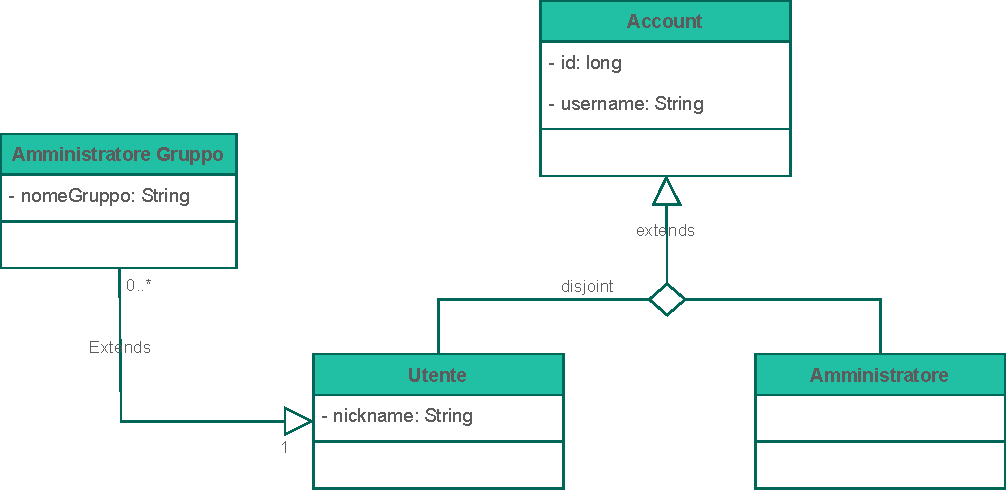
\includegraphics[scale=1]{dominio/Dominio-Struttura Account.drawio.pdf}
\end{adjustwidth}

%------------------------
\pagebreak
\subsubsection*{Area Personale}
\phantomsection
\addcontentsline{toc}{subsection}{Modello del Dominio: Area Personale}
\vspace{0.5cm}
La sezione Area Personale ha come attore l'Utente, il quale usa GestioneFile, GestioneViste, GestioneAccount. Il numero di Viste è limitato a 5, mentre non c'è un limite nel numero di File che è legato solo allo spazio disponibile residuo dell'Utente.
\vspace{0.5cm}

\begin{adjustwidth}{-2cm}{0cm}
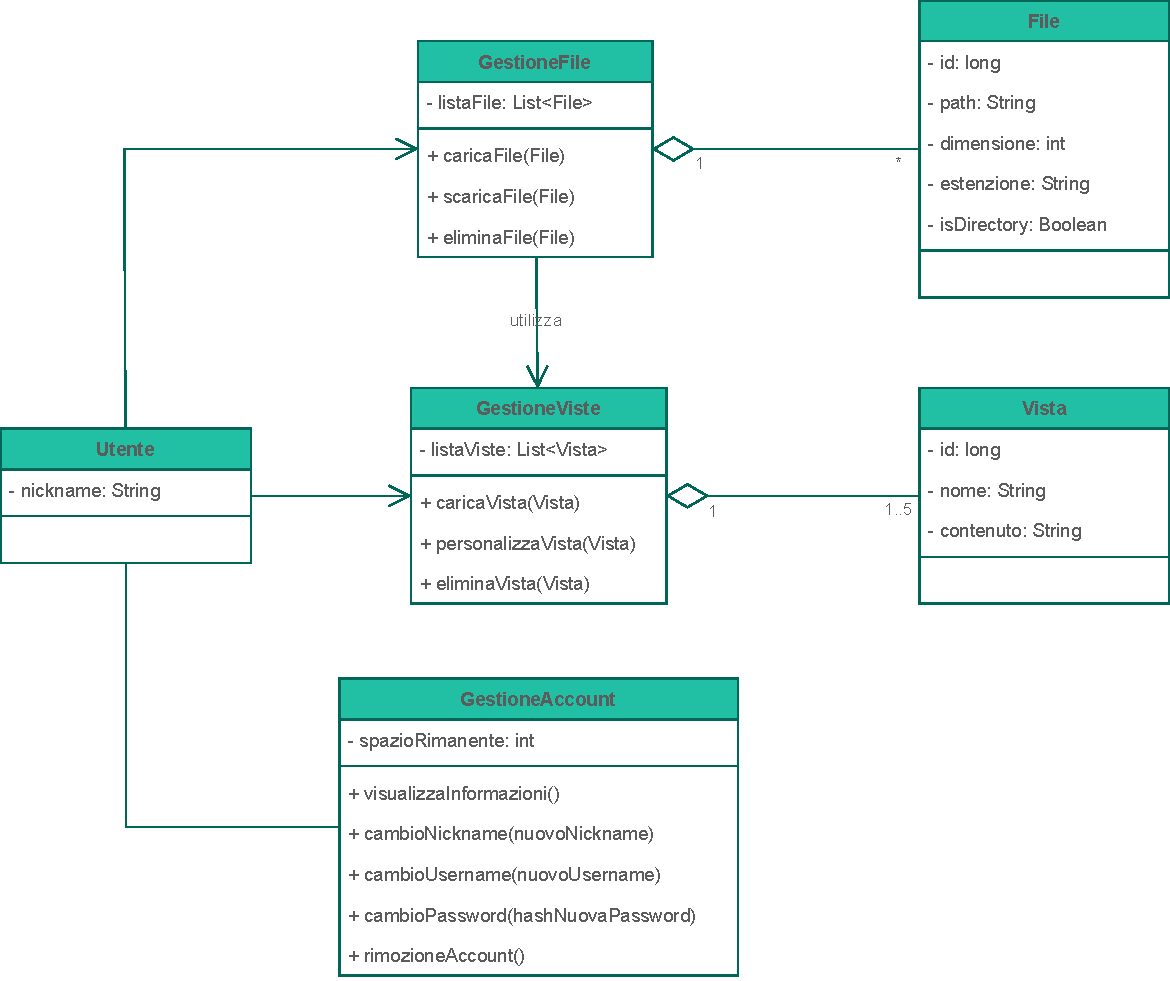
\includegraphics[scale=0.9]{dominio/Dominio-Area Personale.drawio.pdf}
\end{adjustwidth}


%-----------------
\pagebreak
\subsubsection*{Area Gruppi}
\phantomsection
\addcontentsline{toc}{subsection}{Modello del Dominio: Area Gruppi}
\vspace{0.5cm}
Nell' Area Gruppi l'Utente ha a disposizione i metodi per gestire all'interno dei gruppi le proprie risorse e viste. L'Utente dispone anche dei metodi per aggiornare la sua configurazione dell'account tramite GestioneAccount, il quale espone anche lo spazio rimanente.
\vspace{0.5cm}

\begin{adjustwidth}{-2cm}{0cm}
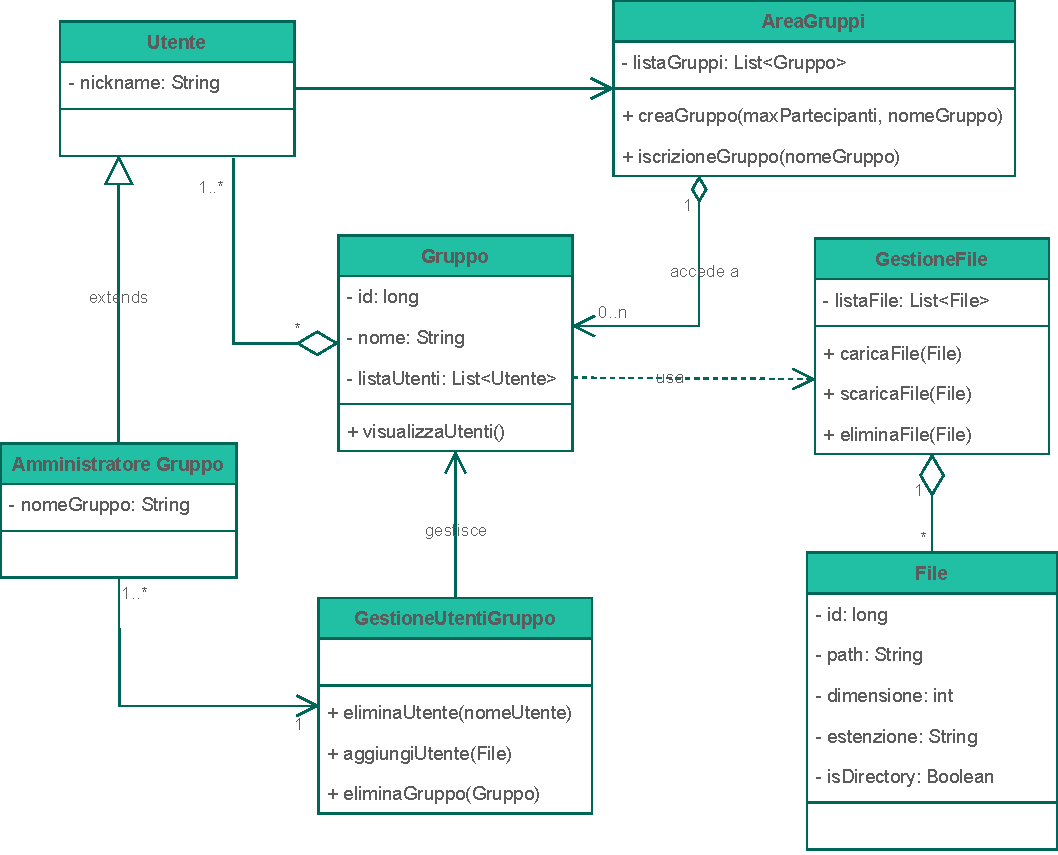
\includegraphics[scale=1]{dominio/Dominio-Area Gruppi.drawio.pdf}
\end{adjustwidth}

%-----------------
\pagebreak
\subsubsection*{Amministrazione}
\phantomsection
\addcontentsline{toc}{subsection}{Modello del Dominio: Amministrazione}
\vspace{0.5cm}

Nella sezione Amministratore, si dispongono i metodi per gestire le richieste.\linebreak \textbf{gestisciRichiestaUtente()} e \textbf{gestisciRichiestaGruppo()} servono per accettare o rifiutare le richieste "in attesa". L'Amministratore può anche eliminare Utenti e Gruppi.Le operazioni sono tracciate registrando nei Logs ogni richiesta.

\vspace{0.5cm}
\begin{adjustwidth}{-2.5cm}{0cm}
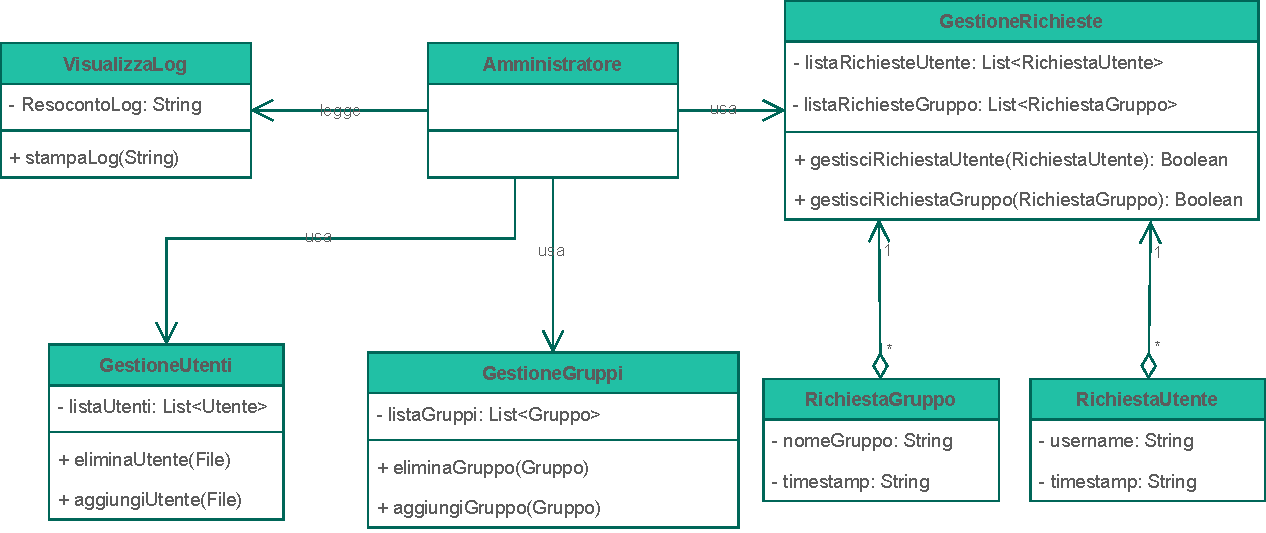
\includegraphics[scale=0.9]{dominio/Dominio-Amministrazione.drawio.pdf}
\end{adjustwidth}
\pagebreak

%------------------
\phantomsection
\addcontentsline{toc}{section}{Architettura Logica: Struttura}
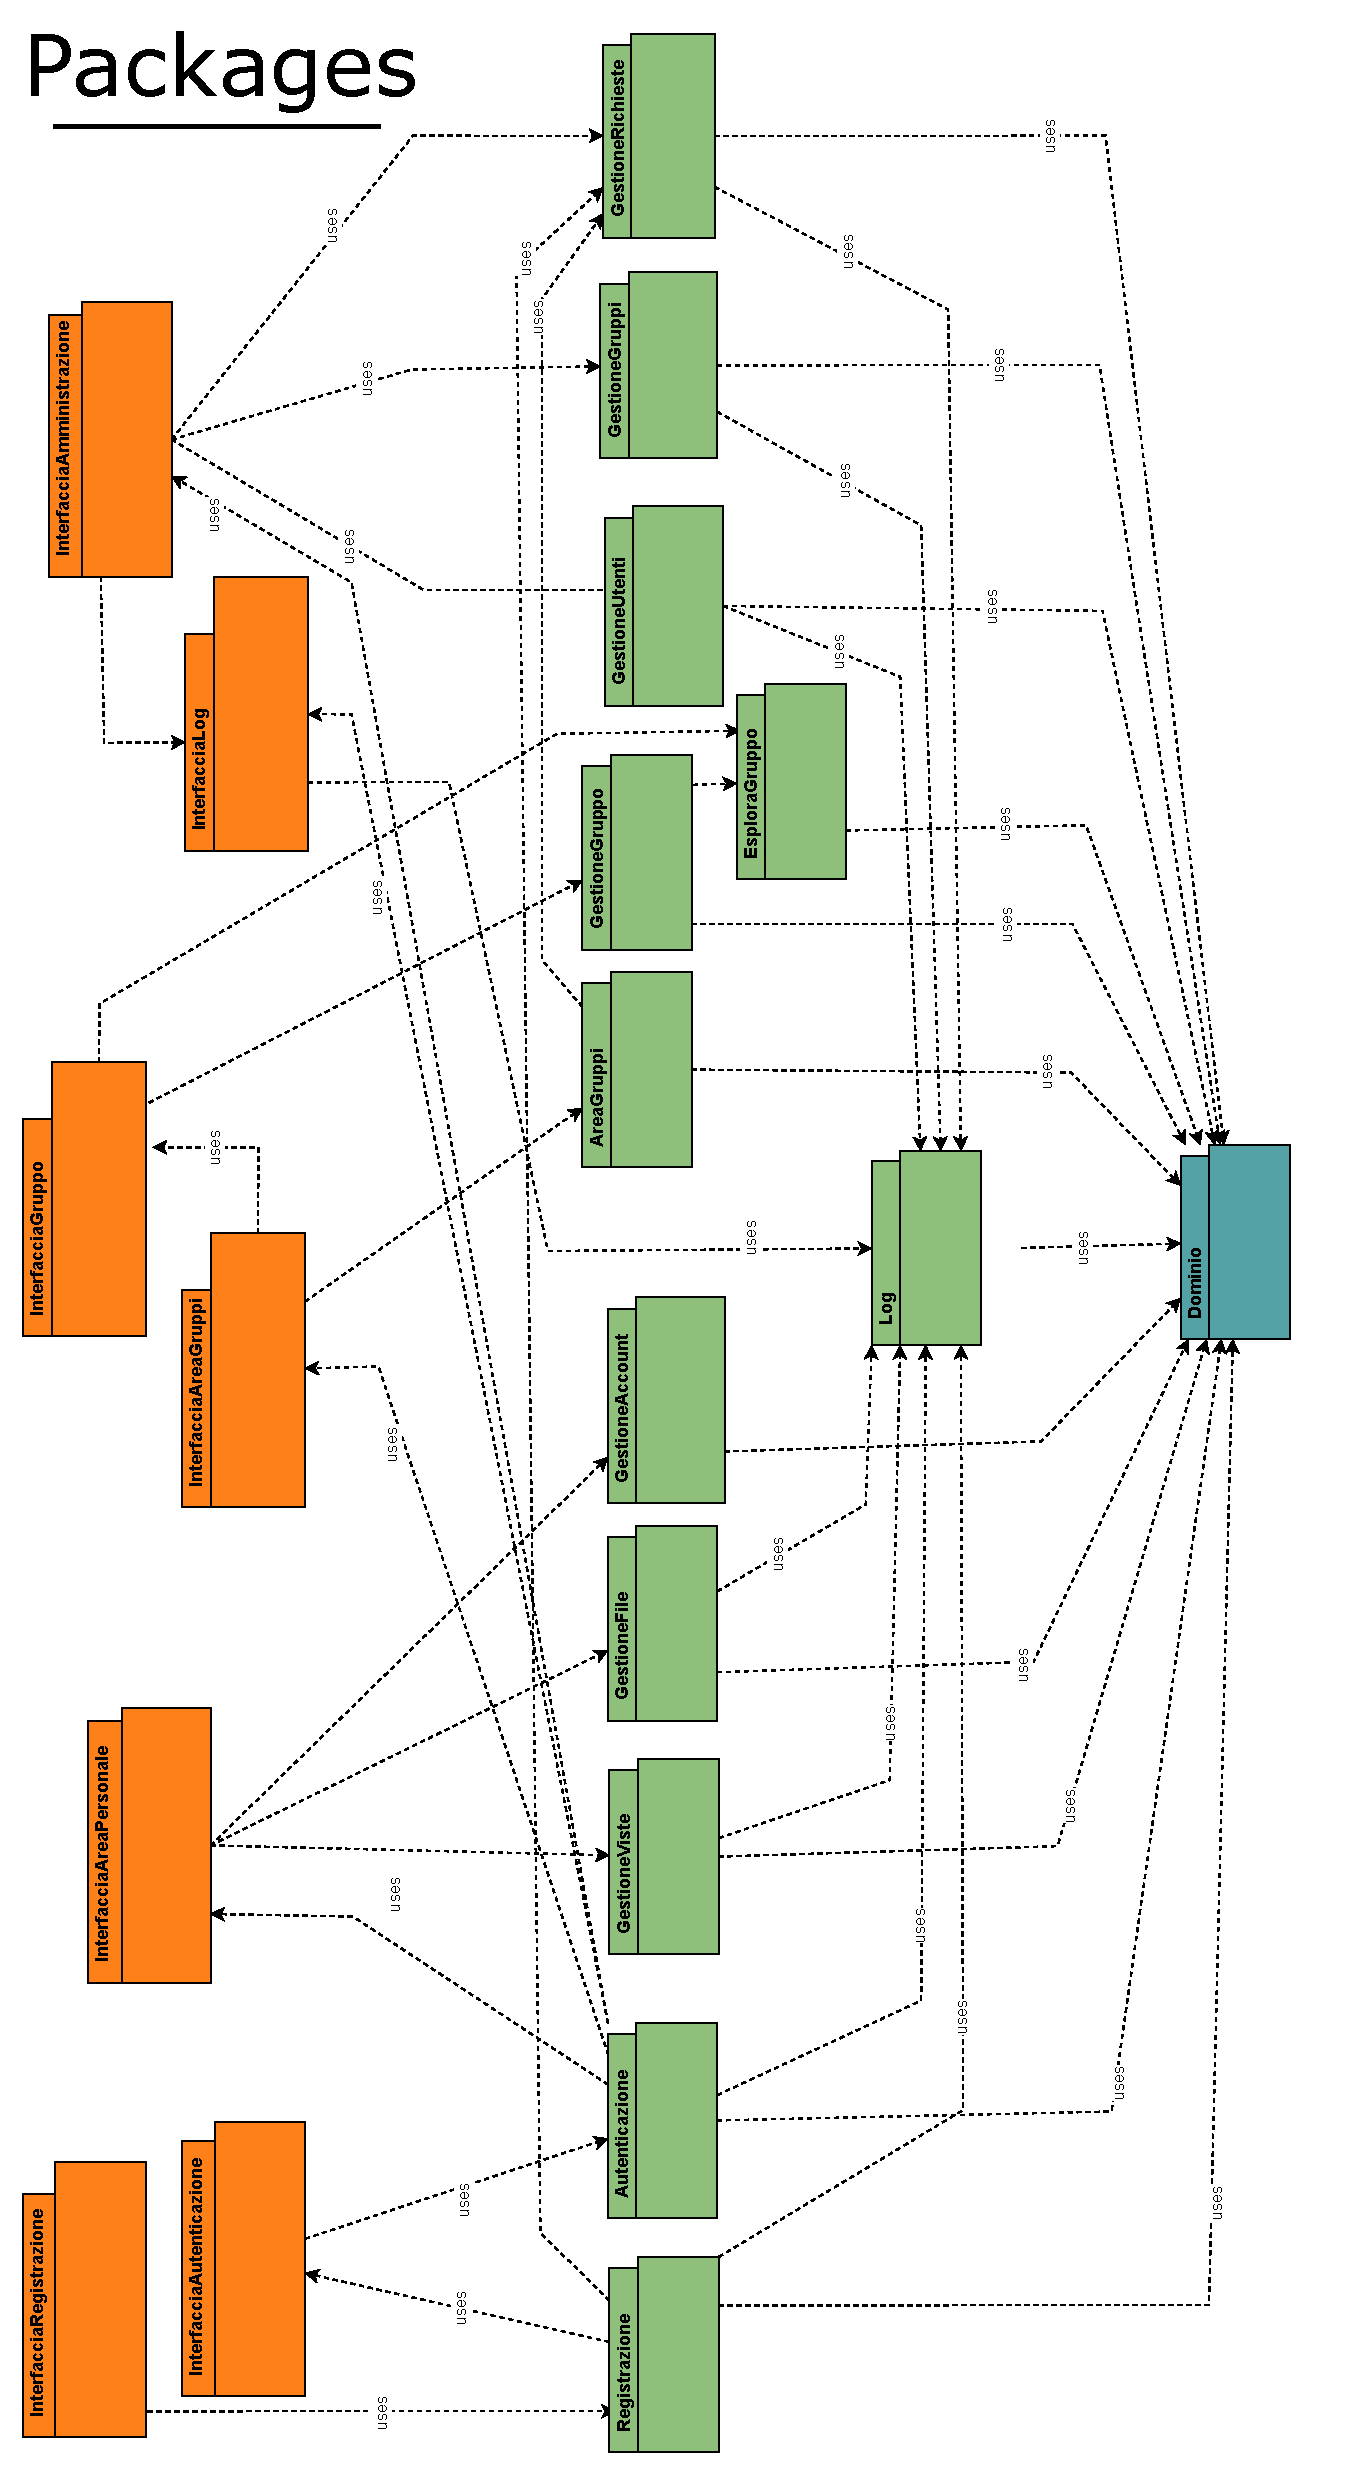
\includepdf[pages={1}]{classi/Package-Package.drawio.pdf}
%-------------------

\subsection*{Diagrammi delle Classi}

\phantomsection
\subsubsection*{Diagramma delle Classi: Autenticazione}
\addcontentsline{toc}{subsection}{Diagramma delle Classi: Autenticazione}
\vspace{1cm}
Il metodo \verb|registraUtente| inserisce la richiesta di registrazione nella \\\verb|listaRichiesteRegistrazione| della classe \verb|GestioneAmministrazioneController|.\\
L' operazione portata a termine quando l'Amministratore accetta la richiesta.
\vspace{2cm}
\begin{adjustwidth}{-2.5cm}{0cm}
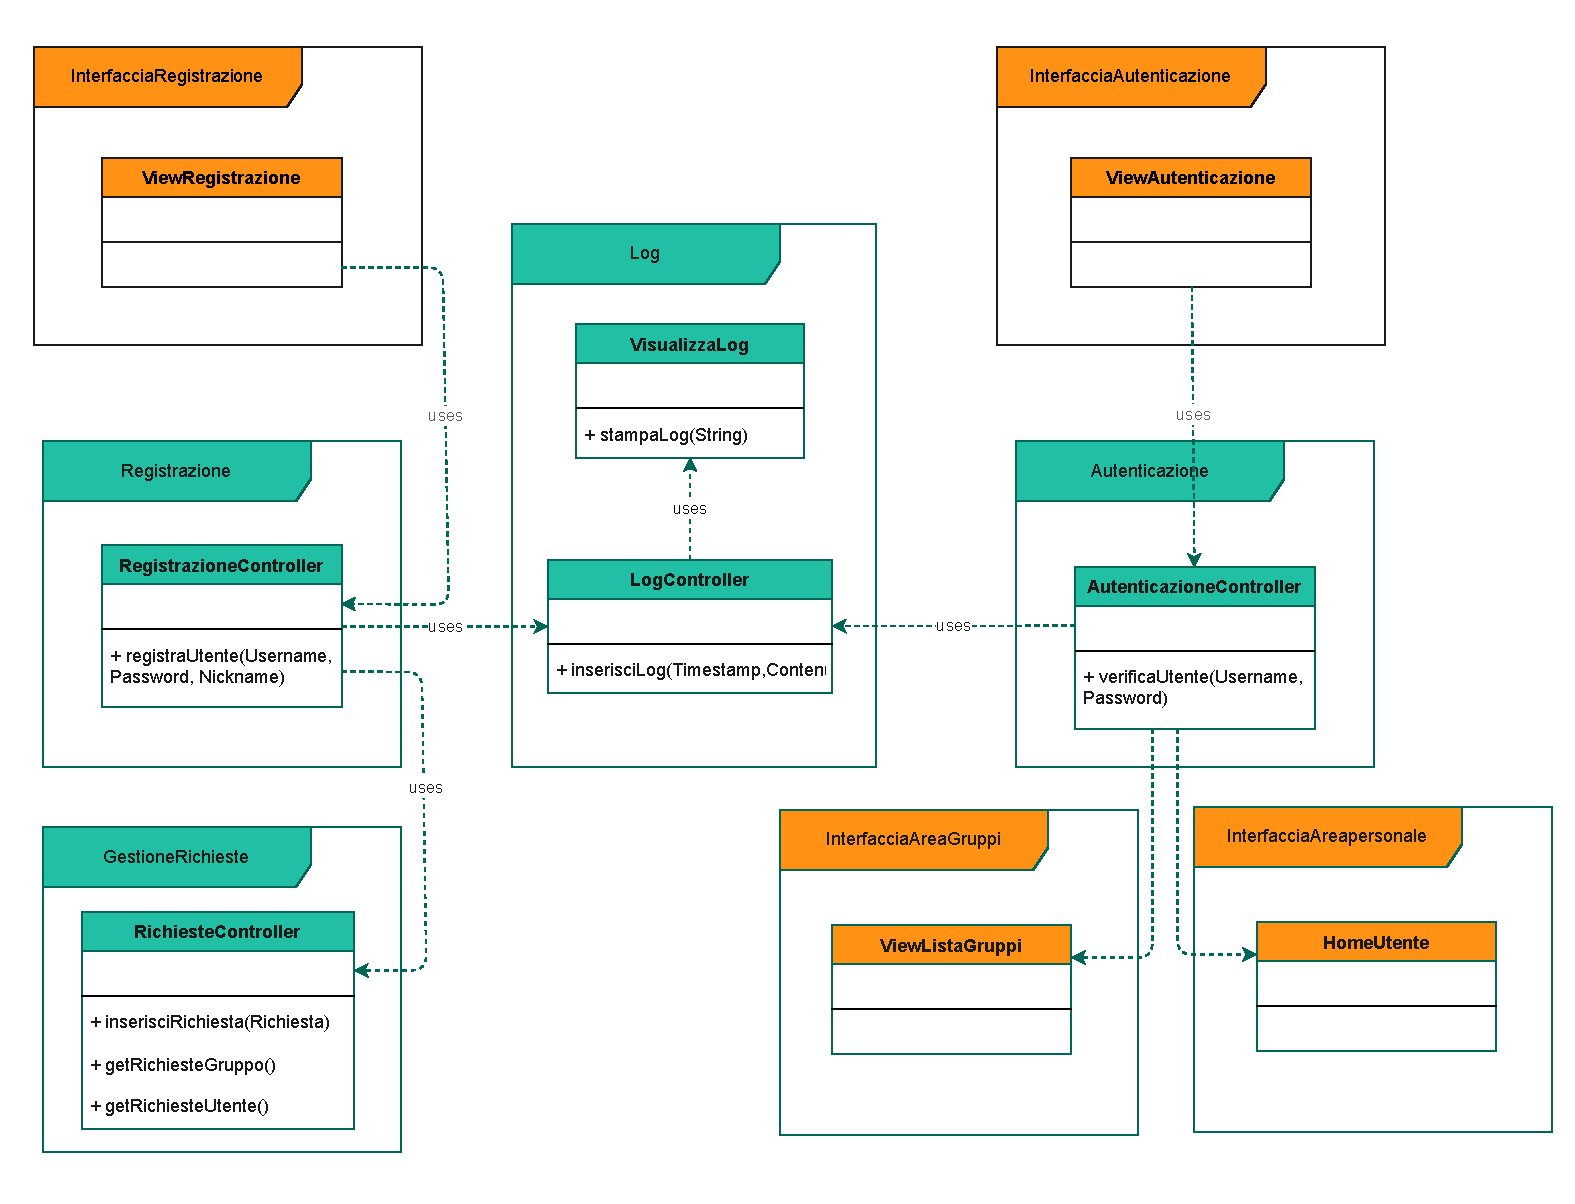
\includegraphics[scale=0.7]{classi/Package-Classi-Autenticazione.drawio.pdf}
\end{adjustwidth}



\phantomsection
\subsubsection*{Diagramma delle Classi: Amministrazione}
\addcontentsline{toc}{subsection}{Diagramma delle Classi: Amministrazione}
\vspace{0.5cm}

\begin{adjustwidth}{-2.5cm}{0cm}
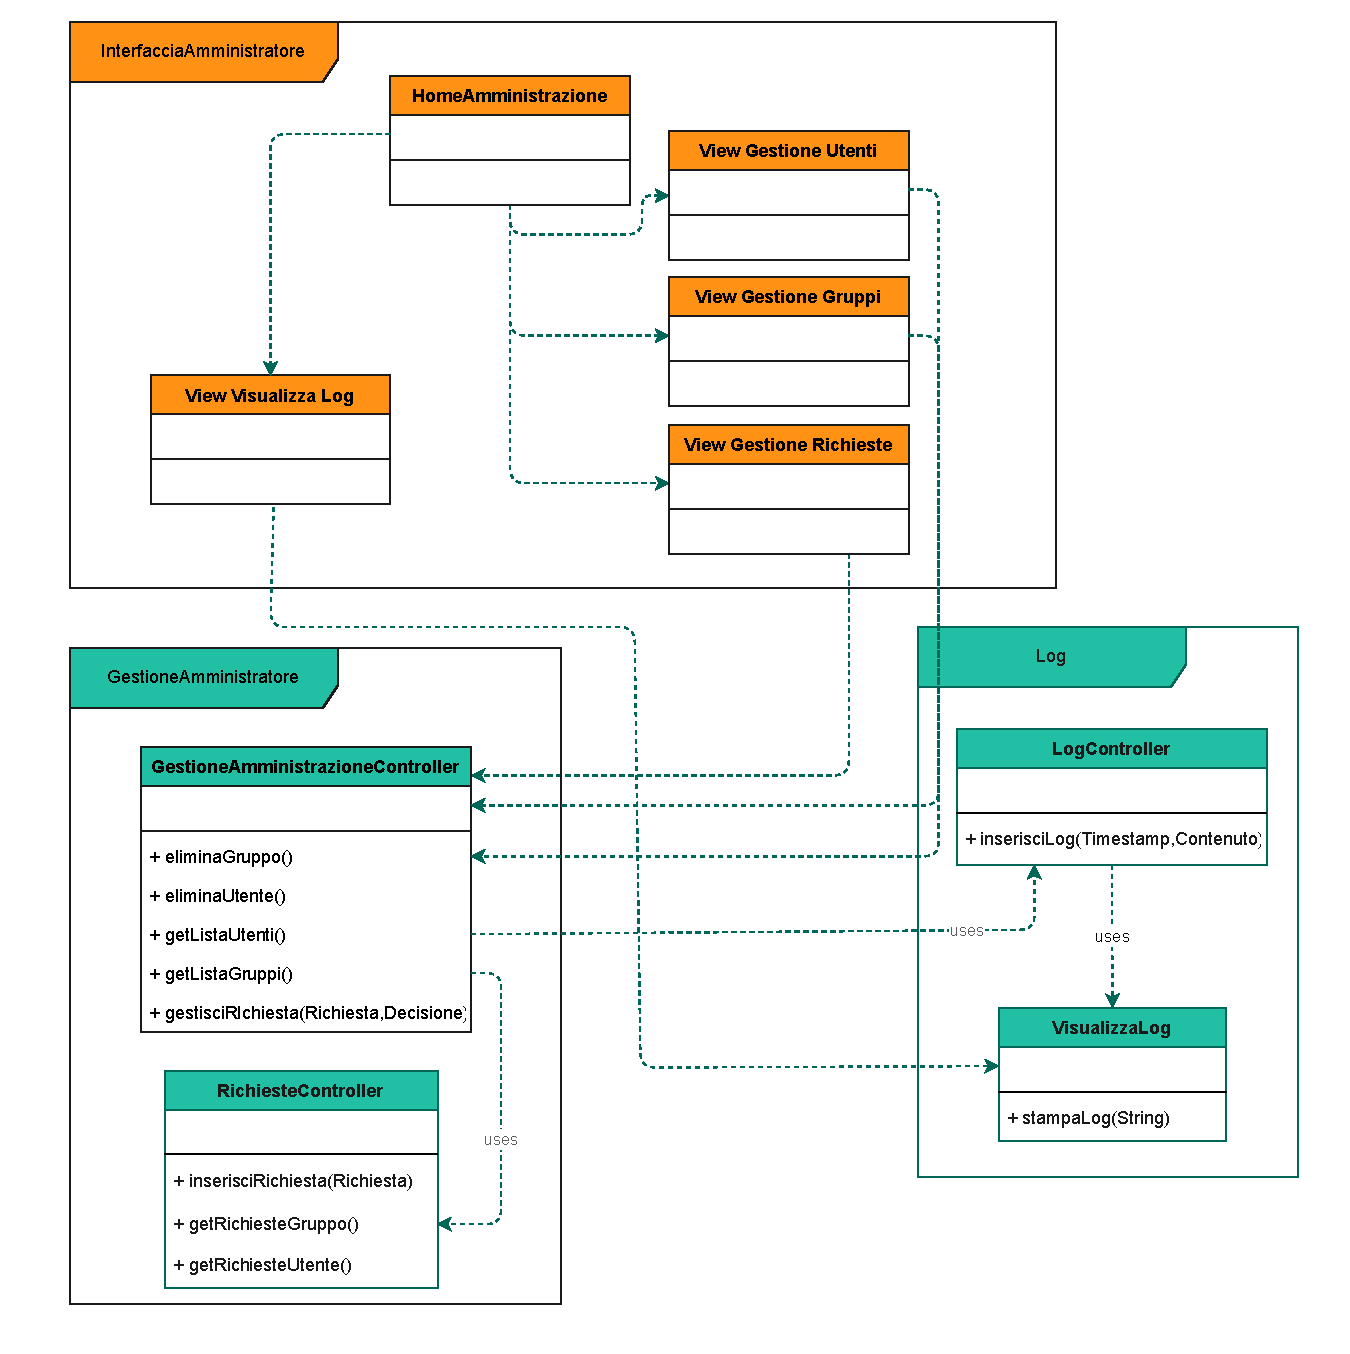
\includegraphics[scale=0.8]{classi/Package-Classi-Amministrazione.drawio.pdf}
\end{adjustwidth}
\vspace{0.5cm}




\phantomsection
\subsubsection*{Diagramma delle Classi: Utente}
\addcontentsline{toc}{subsection}{Diagramma delle Classi: Utente}
\vspace{0.5cm}


\vspace{0.5cm}
\begin{adjustwidth}{-3.5cm}{0cm}
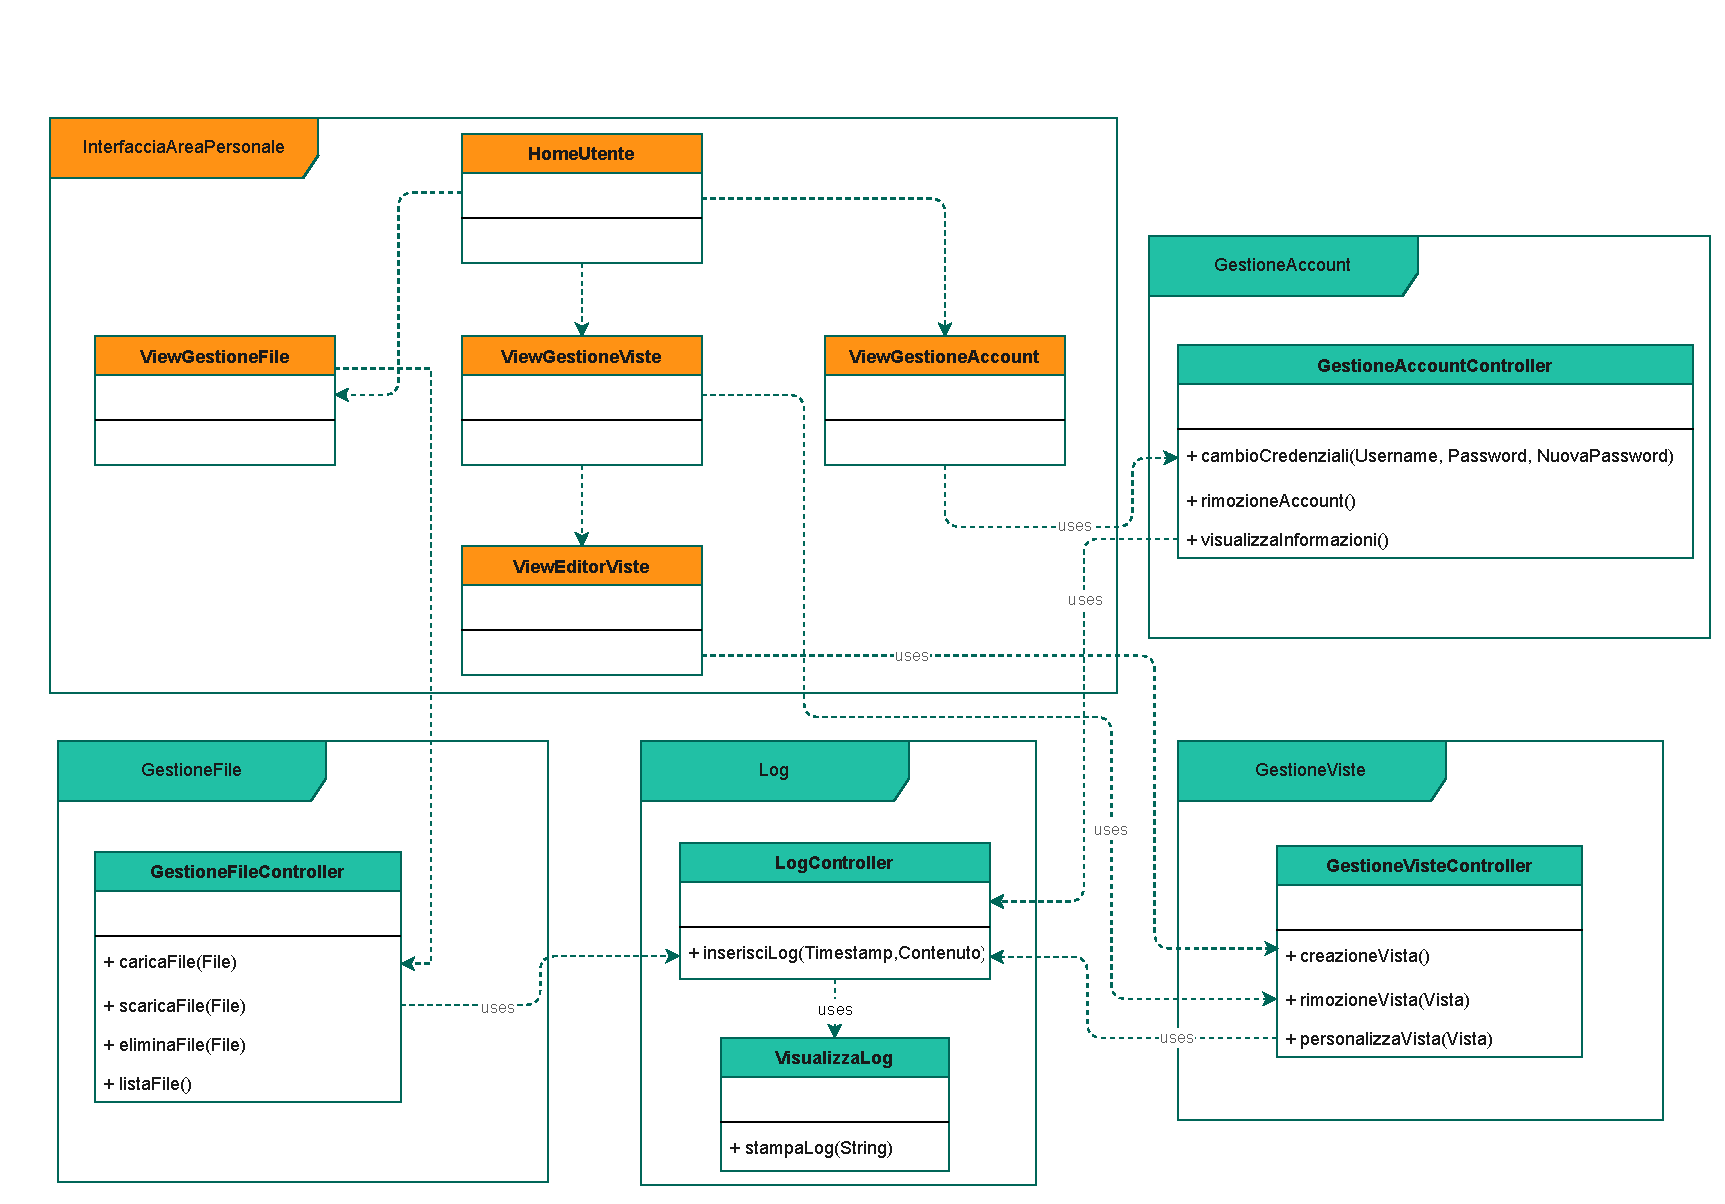
\includegraphics[scale=0.7]{classi/Package-Classi-Utente.drawio.pdf}
\end{adjustwidth}




\phantomsection
\subsubsection*{Diagramma delle Classi: Gruppi}
\addcontentsline{toc}{subsection}{Diagramma delle Classi: Gruppi}
\vspace{0.5cm}


\vspace{0.5cm}
\begin{adjustwidth}{-2.5cm}{0cm}
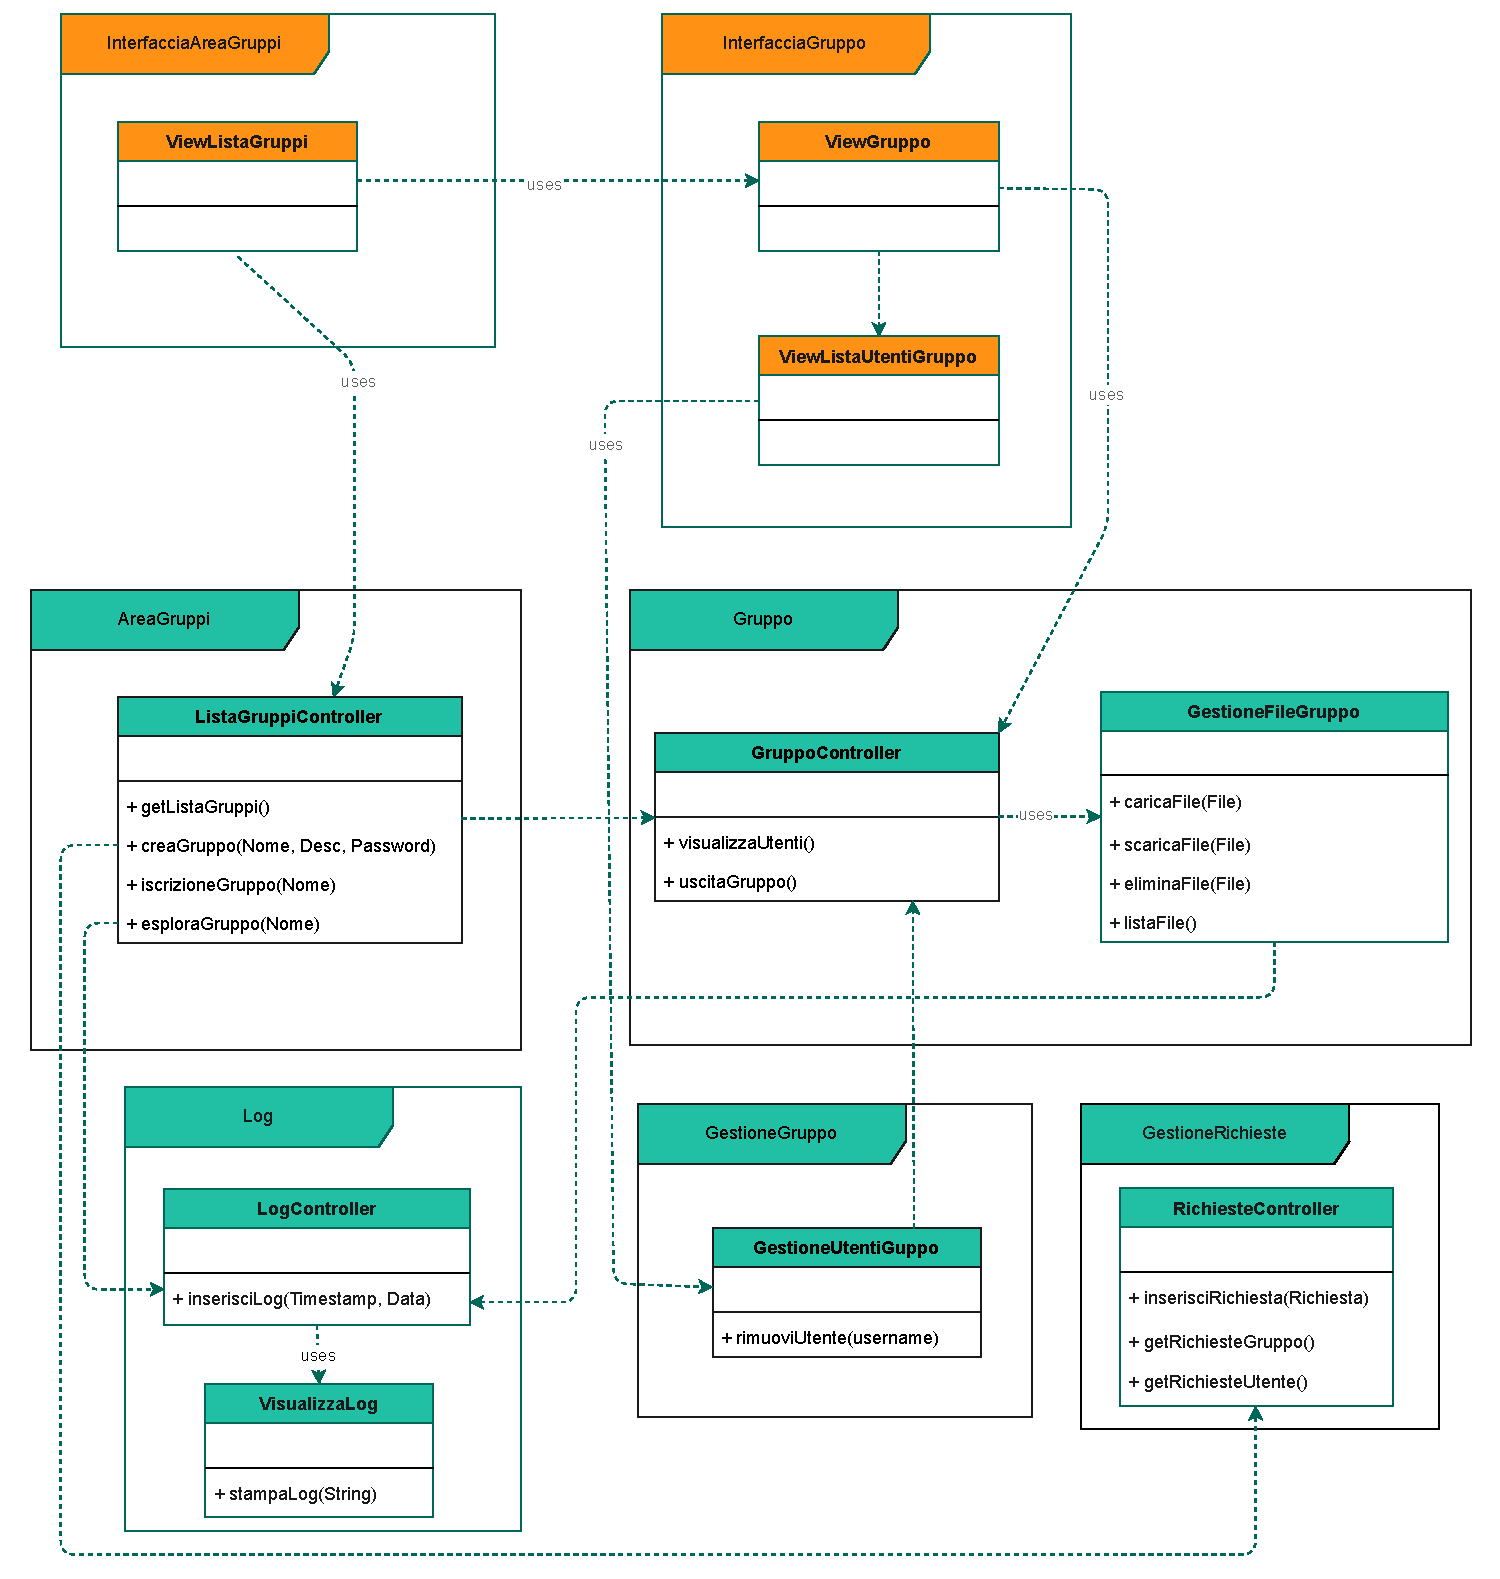
\includegraphics[scale=0.75]{classi/Package-Classi-Gruppi.drawio.pdf}
\end{adjustwidth}



%------------------------------------------


\phantomsection
\section*{Architettura Logica: Interazione}
\addcontentsline{toc}{section}{Architettura Logica: Interazione}
\vspace{0.5cm}


\phantomsection
\subsection*{Diagramma di sequenza : Registrazione}
\addcontentsline{toc}{subsection}{Diagramma di sequenza : Registrazione}
\vspace{0.5cm}

\begin{adjustwidth}{-0.5cm}{0cm}
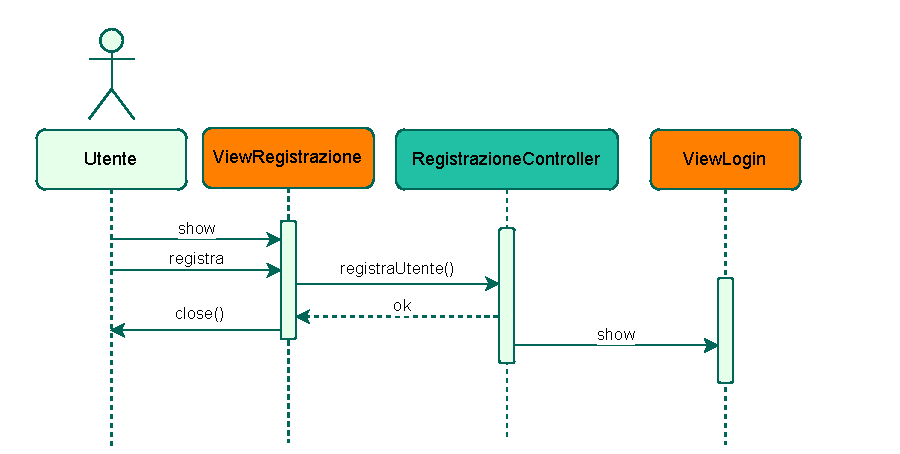
\includegraphics[scale=0.9]{interazione/Package-Interazione-Registrazione.drawio.pdf}
\end{adjustwidth}

\phantomsection
\subsection*{Diagramma di sequenza : Autenticazione}
\addcontentsline{toc}{subsection}{Diagramma di sequenza : Autenticazione}
\vspace{0.5cm}

\begin{adjustwidth}{-0.5cm}{0cm}
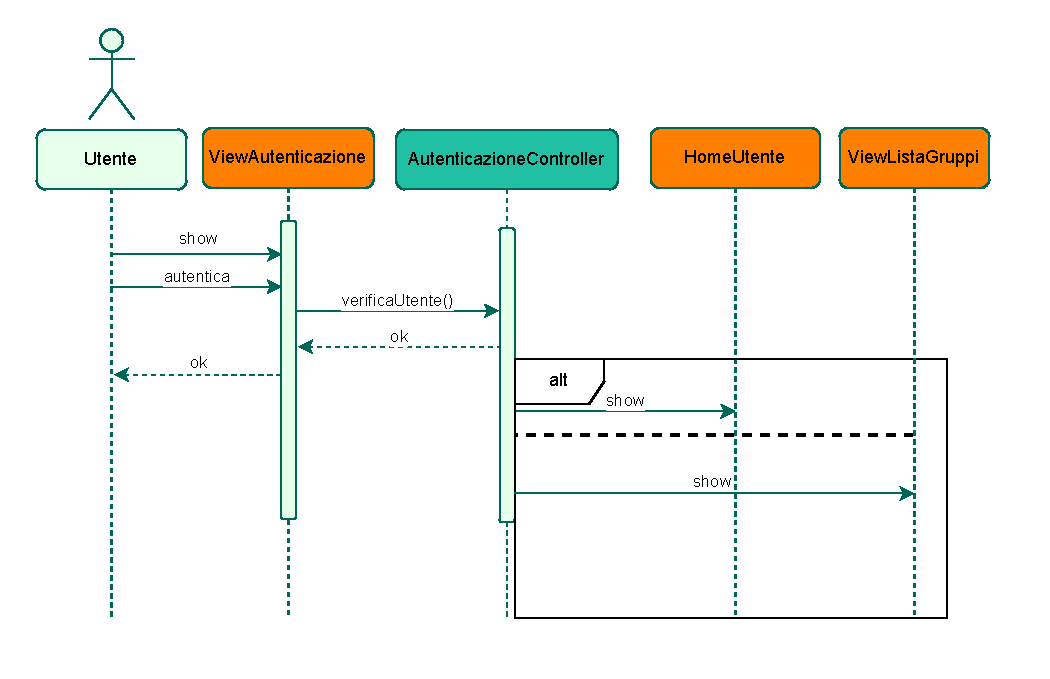
\includegraphics[scale=0.9]{interazione/Package-Interazione-Autenticazione.drawio.pdf}
\end{adjustwidth}


\phantomsection
\subsection*{Diagramma di sequenza : Gestione Amministratore}
\addcontentsline{toc}{subsection}{Diagramma di sequenza : Gestione Amministratore}
\vspace{0.5cm}

\vspace{0.5cm}
\begin{adjustwidth}{-1cm}{0cm}
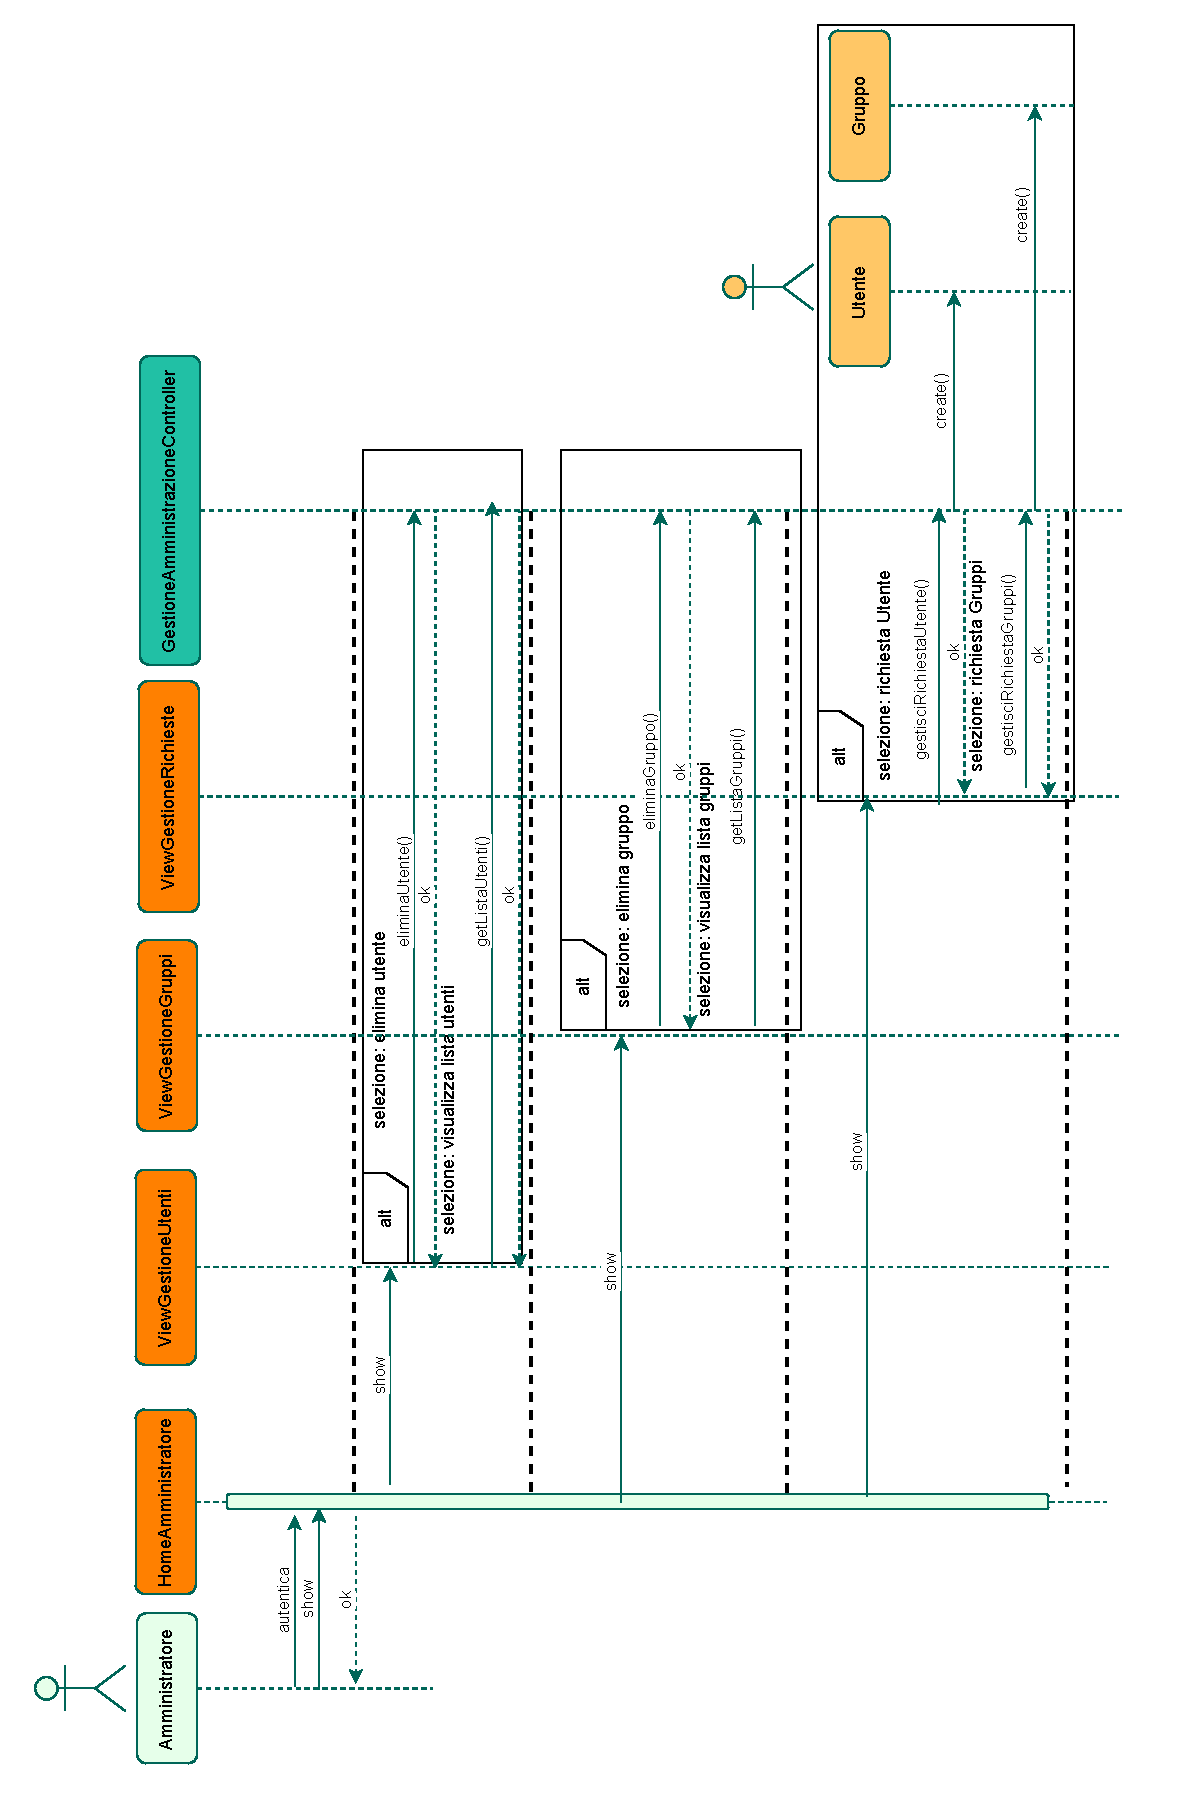
\includegraphics[scale=0.8]{interazione/Package-Interazione-GestioneAmministratore.drawio.pdf}
\end{adjustwidth}

\phantomsection
\subsubsection*{Diagramma di sequenza : Area Personale\-Viste}
\addcontentsline{toc}{subsection}{Diagramma di sequenza : Area Personale\-Viste}
\vspace{0.5cm}

\begin{adjustwidth}{-2.5cm}{0cm}
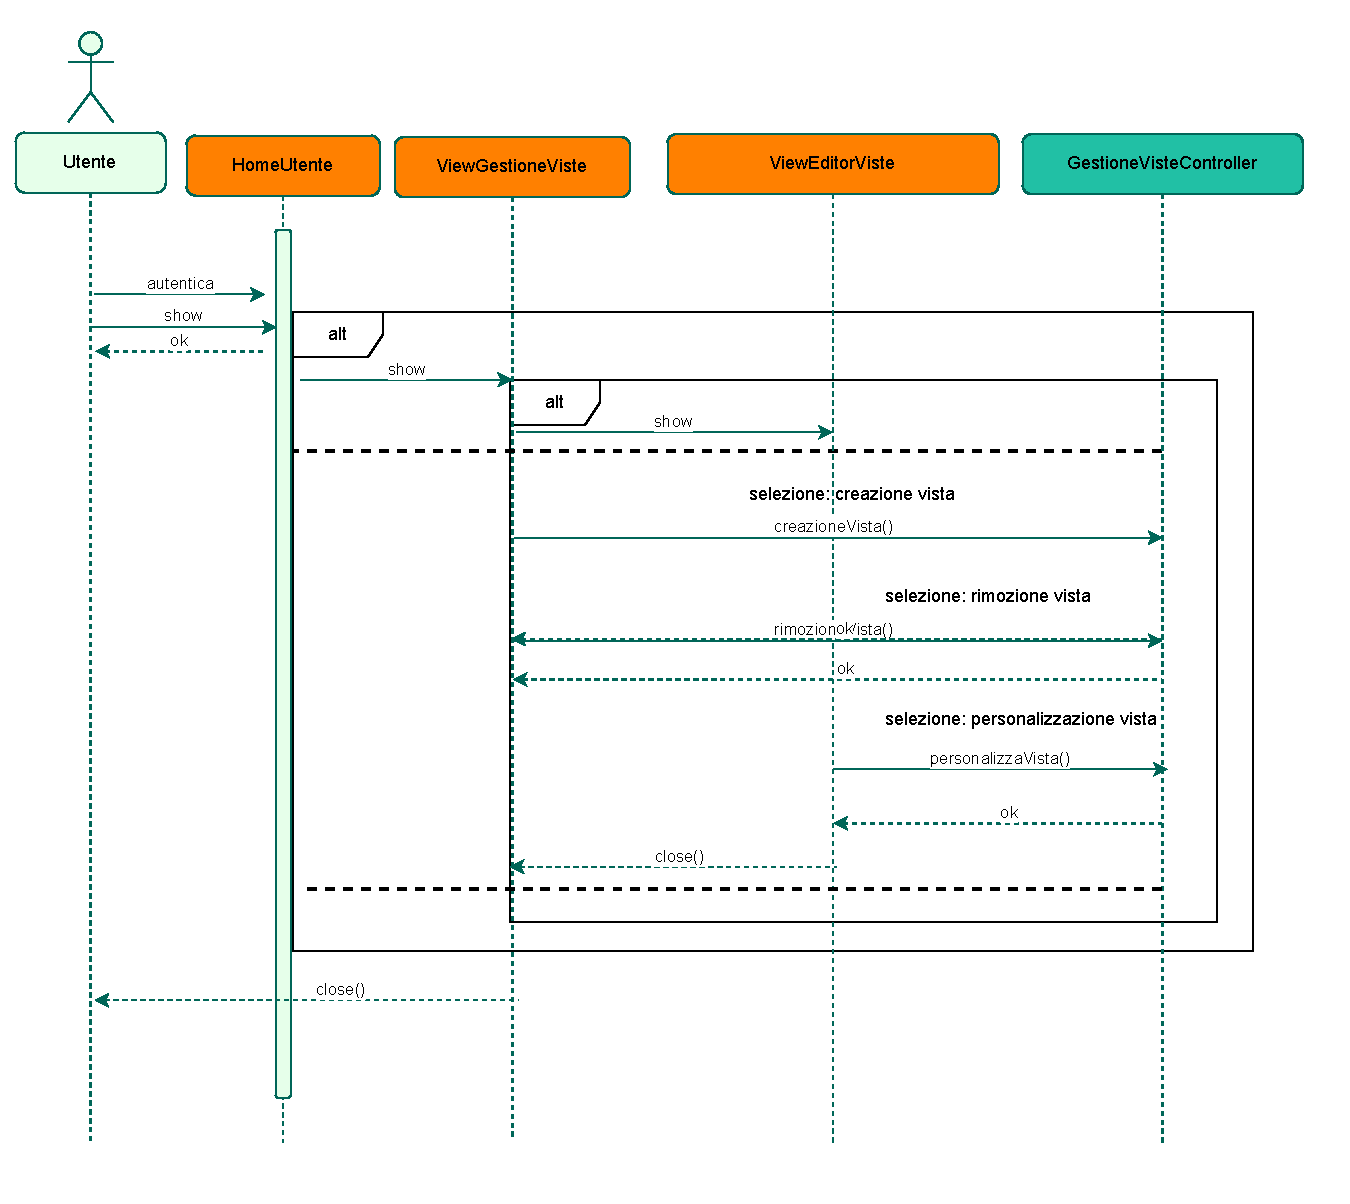
\includegraphics[scale=0.8]{interazione/Package-Interazione-AreaPersonale.drawio.pdf}
\end{adjustwidth}


\phantomsection
\subsubsection*{Diagramma di sequenza : Area Gruppi}
\addcontentsline{toc}{subsection}{Diagramma di sequenza : Area Gruppi}
\vspace{0.5cm}

\begin{adjustwidth}{-2.5cm}{0cm}
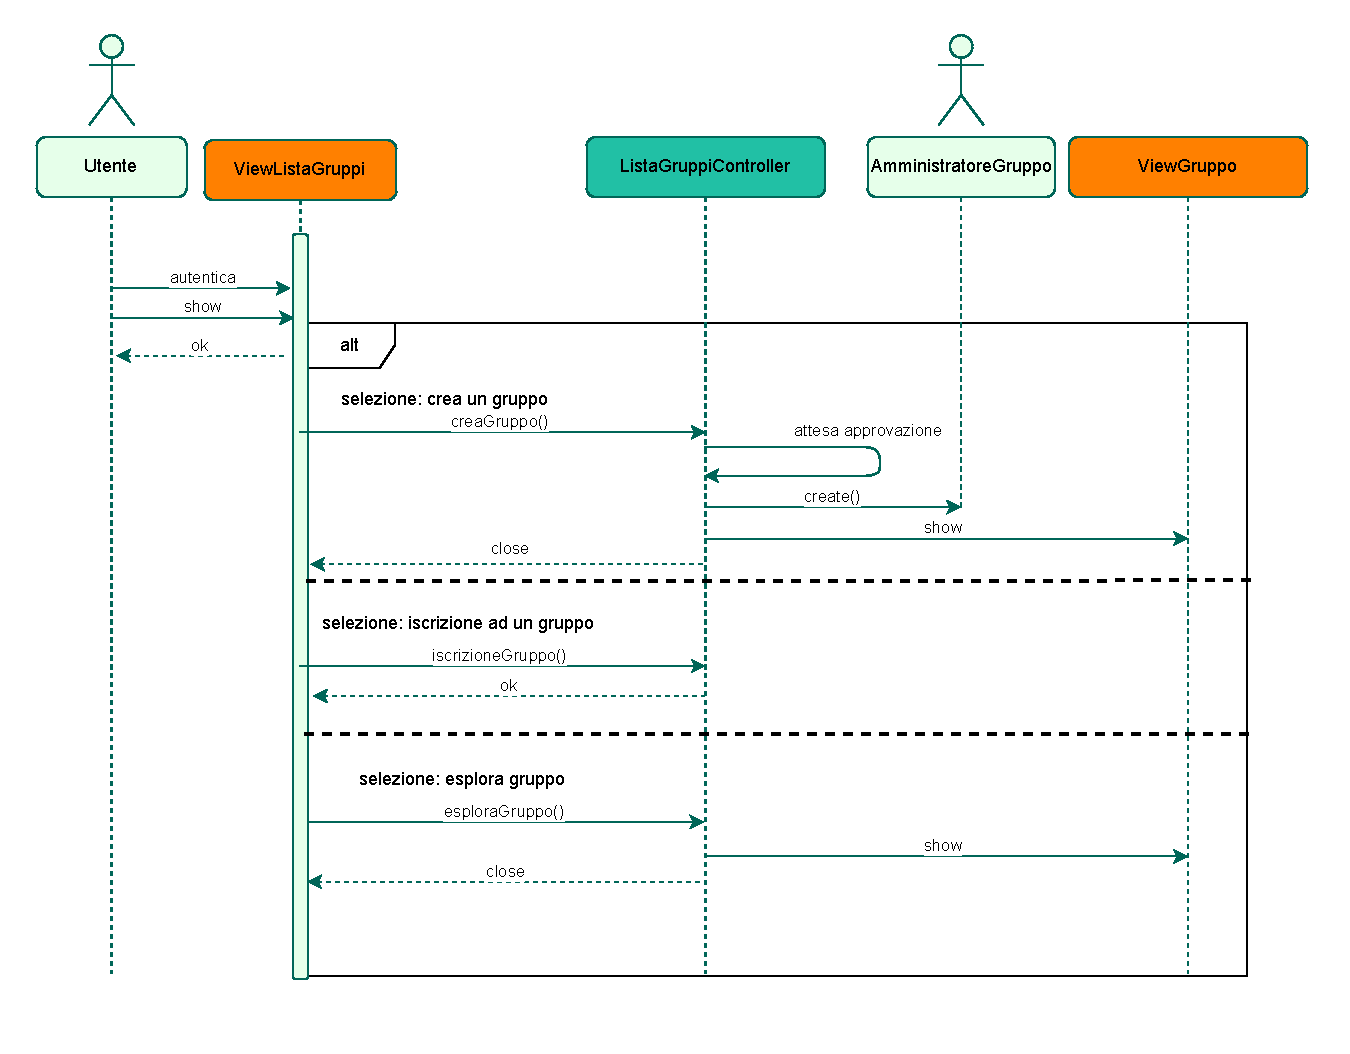
\includegraphics[scale=0.8]{interazione/Package-Interazione-AreaGruppi.drawio.pdf}
\end{adjustwidth}


\pagebreak
\pagebreak
\phantomsection
\section*{Piano di Lavoro}
\addcontentsline{toc}{section}{Piano di Lavoro}
\vspace{0.5cm}

Si è deciso di dividere sviluppo e progetto tra i vari membri nel seguente modo: 
\\ \\

\rowcolors{2}{white!0!}{white!0!}
\begin{adjustwidth}{-0.5cm}{0cm}
\resizebox{1.1\textwidth}{!}{
\begin{tabular}{ |l|c|c| }
\hline
\rowcolor{purple!25}\Large\textbf{Package} & \Large\textbf{Progetto} & \Large\textbf{Sviluppo} \\
\hline
InterfacciaRegistrazione & Nanni Cirulli, Venerandi, Di Fazio & Venerandi, Di Fazio\\
\hline
InterfacciaAutenticazione & Nanni Cirulli, Venerandi, Di Fazio & Venerandi, Di Fazio\\
\hline
InterfacciaAreaPersonale & Nanni Cirulli, Venerandi, Di Fazio & Nanni Cirulli\\
\hline
InterfacciaAreaGruppi & Nanni Cirulli, Venerandi, Di Fazio & Venerandi\\
\hline
InterfacciaGruppo & Nanni Cirulli, Venerandi, Di Fazio &  Venerandi\\
\hline
InterfacciaLog & Nanni Cirulli, Venerandi, Di Fazio &  Nanni Cirulli\\
\hline
InterfacciaAmministratore & Nanni Cirulli, Venerandi, Di Fazio &  Di Fazio\\
\hline
Registrazione & Nanni Cirulli, Venerandi, Di Fazio &  Venerandi, Di Fazio\\
\hline
Autenticazione & Nanni Cirulli, Venerandi, Di Fazio &  Venerandi, Di Fazio\\
\hline
GestioneViste & Nanni Cirulli, Venerandi, Di Fazio &  Nanni Cirulli, Di Fazio\\
\hline
GestioneFile & Nanni Cirulli, Venerandi, Di Fazio &  Nanni Cirulli, Di Fazio\\
\hline
GestioneAccount & Nanni Cirulli, Venerandi, Di Fazio &  Di Fazio\\
\hline
Log & Nanni Cirulli, Venerandi, Di Fazio &  Nanni Cirulli\\
\hline
AreaGruppi & Nanni Cirulli, Venerandi, Di Fazio &  Nanni Cirulli, Venerandi \\
\hline
GestioneGruppo & Nanni Cirulli, Venerandi, Di Fazio &  Venerandi, Di Fazio\\
\hline
EsploraGruppo & Nanni Cirulli, Venerandi, Di Fazio &  Di Fazio\\
\hline
GestioneUtenti & Nanni Cirulli, Venerandi, Di Fazio &  Venerandi, Di Fazio\\
\hline
GestioneGruppi & Nanni Cirulli, Venerandi, Di Fazio &  Venerandi, Nanni Cirulli\\
\hline
GestioneRichieste & Nanni Cirulli, Venerandi, Di Fazio &  Nanni Cirulli, Venerandi, Di Fazio\\
\hline
\end{tabular}
}
\end{adjustwidth}
\vspace{0.5cm}


\phantomsection
\subsection*{Prototipo}
\addcontentsline{toc}{subsection}{Prototipo}

Il prototipo prevederà la possibilità di registrarsi e autenticarsi, di gestire il pannello come amministratore e di utilizzare l'Area Personale per accedere alla sezione di Gestione File, dove sarà possibile caricare i file. Nell' interfaccia delle viste sarà invece possibile predisporre i file secondo una delle viste selezionate.

\vspace{0.3cm}
\phantomsection
\subsection*{Sviluppi Futuri}
\addcontentsline{toc}{subsection}{Sviluppi Futuri}

Nelle versioni successive dell' applicazione si potrà avere un numero maggiore di viste preimpostate, una gestione dell' account completa con più funzionalità e l'amministratore di gruppo avrà dei pannelli di gestione completi.


\pagebreak
\phantomsection
\subsection*{Piano del collaudo}
\addcontentsline{toc}{subsection}{Piano del collaudo}

Per gestire lo sviluppo dell' applicazione sono stati predisposti alcuni test per analizzare il comportamento di componenti specifici del sistema. Nelle pagine successive vengono riportati parte dei test effettuati sul sistema. 

\inputminted
[
frame=lines,
framesep=2mm,
baselinestretch=1.2,
bgcolor=opal!20!,
fontsize=\footnotesize,
linenos
]
{csharp}{code/test.cs}


\chapter*{Progettazione}
\addcontentsline{toc}{chapter}{Progettazione}
\phantomsection
\section*{Progettazione architetturale}
\addcontentsline{toc}{section}{Progettazione architetturale}
\vspace{0.5cm}

\phantomsection
\subsection*{Requisiti non Funzionali}
\addcontentsline{toc}{subsection}{Requisiti non Funzionali}
\vspace{0.5cm}
Nell' Analisi del problema sono emersi dei requisiti non funzionali che impongono i seguenti vincoli:

\begin{enumerate}
\item Interfaccia utente intuitiva.
\item Velocità nel caricare/scaricare file.
\item Organizzazione del file manager ampiamente personalizzabile.
\item Possibilità di cambiare la view in modo rapido.
\item Utilizzo efficace del servizio anche in assenza di una connessione veloce.
\item Pannello di amministrazione intuitivo
\end{enumerate}

\\
L'interfaccia utente deve permettere di far capire immediatamente all'utente le funzionalità disponibili per caricare e scaricare file, inoltre deve essere fornito un sistema facile e veloce per modificare le varie viste. L'utilizzo veloce è garantito anche in assenza di una connessione veloce, perché le operazioni sulle viste verranno svolte principalmente lato client.\\
Il pannello di amministrazione intuitivo permetterà all'amministratore di operare velocemente nel sistema, agendo tempestivamente sugli utenti che svolgono azioni indesiderate.


\phantomsection
\subsection*{Scelta dell' Architettura}
\addcontentsline{toc}{subsection}{Scelta dell' Architettura}
Per l'architettura del sistema si è optato per un sistema Client/Server che si appoggia ad un Database. Le connessioni tra i vari livelli saranno cifrate.
\vspace{0.5cm}
\phantomsection
\subsection*{L1 - Client}
\addcontentsline{toc}{subsection}{L1 - Client}
Il Client utilizzerà una connessione TLS che sarà fondamentale in tutte le operazioni di interazione con il server e per lo scambio dei file che avverrà tra i due.
Per aggiungere un ulteriore livello di sicurezza, negli sviluppi futuri dell' applicazione si potrebbe aggiungere una cifratura dei file lato server.
\\
Il Client Utente sarà potenzialmente anche Client AmministratoreGruppo e sarà poi presente un Client Amministratore separato.
\vspace{0.5cm}

\phantomsection
\subsection*{L2 - Server}
\addcontentsline{toc}{subsection}{L2 - Server}
\vspace{0.5cm}
Sul sistema sarà presente
\begin{itemize}
\item Un Server per la gestione degli Utenti
\item Un Server per la gestione dei Gruppi
\item Un Server per la gestione degli Amministratori
\item Un Server per la gestione dei File
\end{itemize}
\phantomsection
\subsection*{L3 - Database}
\addcontentsline{toc}{subsection}{L3 - Database}
Per la gestione della persistenza dei dati degli Utenti e dell' Amministratore e per salvare gli ID dei file, viene utilizzata una connessione sicura TLS già supportata dal database e in più verrà aggiunto un SALT che garantirà una maggiore sicurezza nel caso di attacchi a dizionario.
Il Database - Server sarà installabile in modo disaccoppiato al sistema, in modo da poter utilizzare anche eventualmente un sistema Cloud o un sistema esterno per salvare i dati.
\\
Il database sarà disposto su tre server: un database memorizzerà i dati degli utilizzatori del sistema, un altro database memorizzerà i LOG e sarà accessibile dall'Amministratore per il monitoraggio del sistema e l'ultimo database manterrà la struttura ad albero dei file con i relativi ID.
Questo disaccoppiamento è utile per non avere un "Single Point of Failure" che può avvenire tramite un guasto all'unico sistema di persistenza, ad esempio non sarebbe tollerabile un disservizio al database degli utenti causato da un malfunzionamento del database dei LOG.
\\
L'interfacciamento fra l'applicativo e i DBMS avverrà secondo la metodologia \verb|forza bruta|, utilizzando dei metodi CRUD.

\vspace{0.5cm}

\phantomsection
\subsection*{Scelte Tecnologiche}
\addcontentsline{toc}{subsection}{Scelte Tecnologiche}

L'applicazione viene sviluppata come applicazione web, in modo da essere accessibile da molti dispositivi che supportano le tecnologie web moderne e abbiano a disposizione un web browser.
\\
Per l'installazione può essere utilizzato un metodo "a container" che faciliterà il deploy, oltre che a rendere più chiusa l'applicazione verso il sistema principale.

\vspace{0.5cm}

\pagebreak
\phantomsection
\subsection*{Diagramma dei package}
\addcontentsline{toc}{subsection}{Diagramma dei package}
Di seguito è riportata l’Architettura del Sistema organizzata attraverso un diagramma dei package.
\vspace{2cm}

\begin{adjustwidth}{-3cm}{0cm}
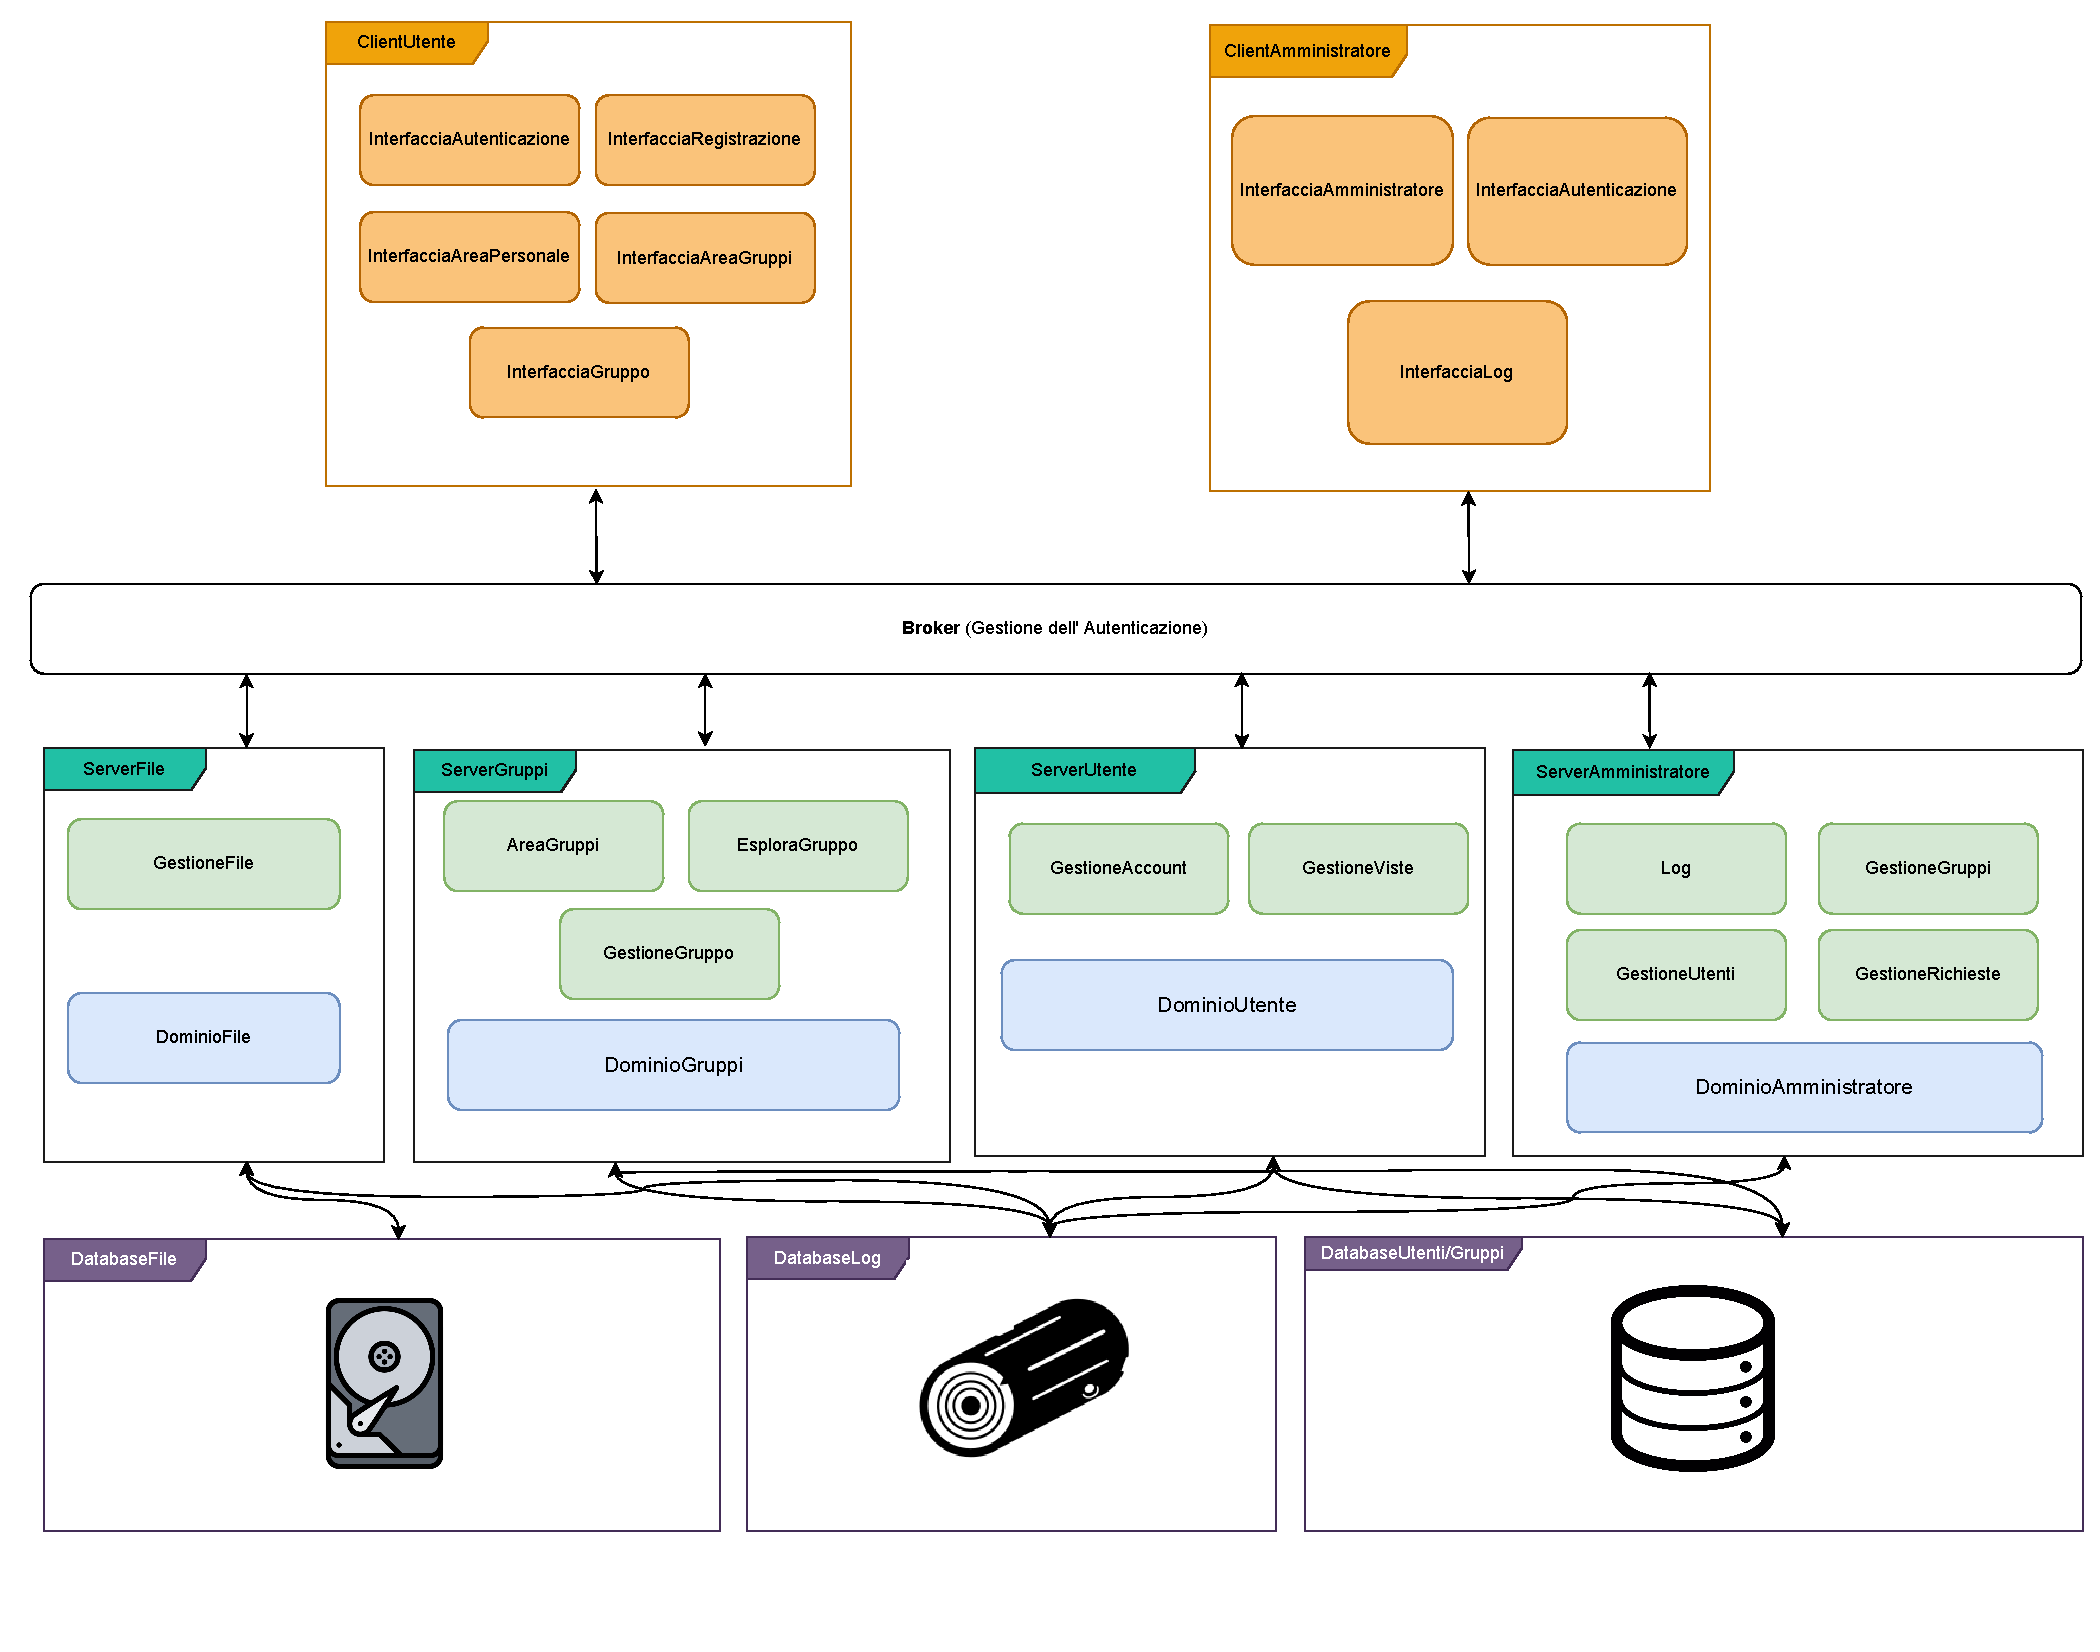
\includegraphics[scale=0.55]{progettazione/Progettazione-Diagramma Package.drawio.pdf}
\end{adjustwidth}


\pagebreak
\phantomsection
\subsection*{Diagramma dei componenti}
\addcontentsline{toc}{subsection}{Diagramma dei componenti}
Di seguito è riportato il diagramma dei componenti di sistema.
\vspace{2cm}
\begin{adjustwidth}{1cm}{0cm}
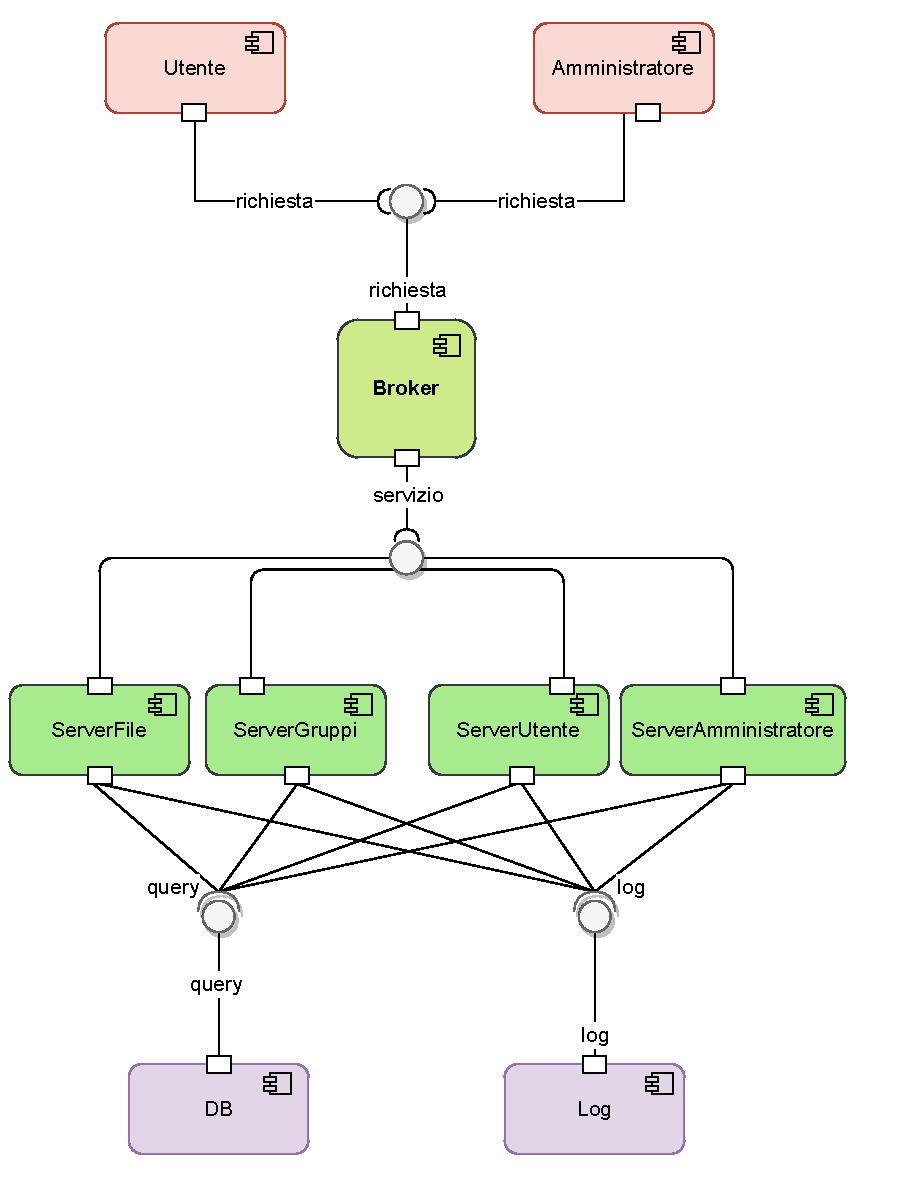
\includegraphics[scale=0.9]{progettazione/Progettazione-Diagramma Componenti.drawio.pdf}
\end{adjustwidth}
\vspace{1cm}


\pagebreak
\phantomsection
\section*{Progettazione di dettaglio}
\addcontentsline{toc}{section}{Progettazione di dettaglio}
\vspace{1cm}

\subsection*{Dominio: Struttura Account}
\phantomsection
\addcontentsline{toc}{subsection}{Dominio: Struttura Account}
\vspace{0.5cm}
\begin{adjustwidth}{-2cm}{0cm}
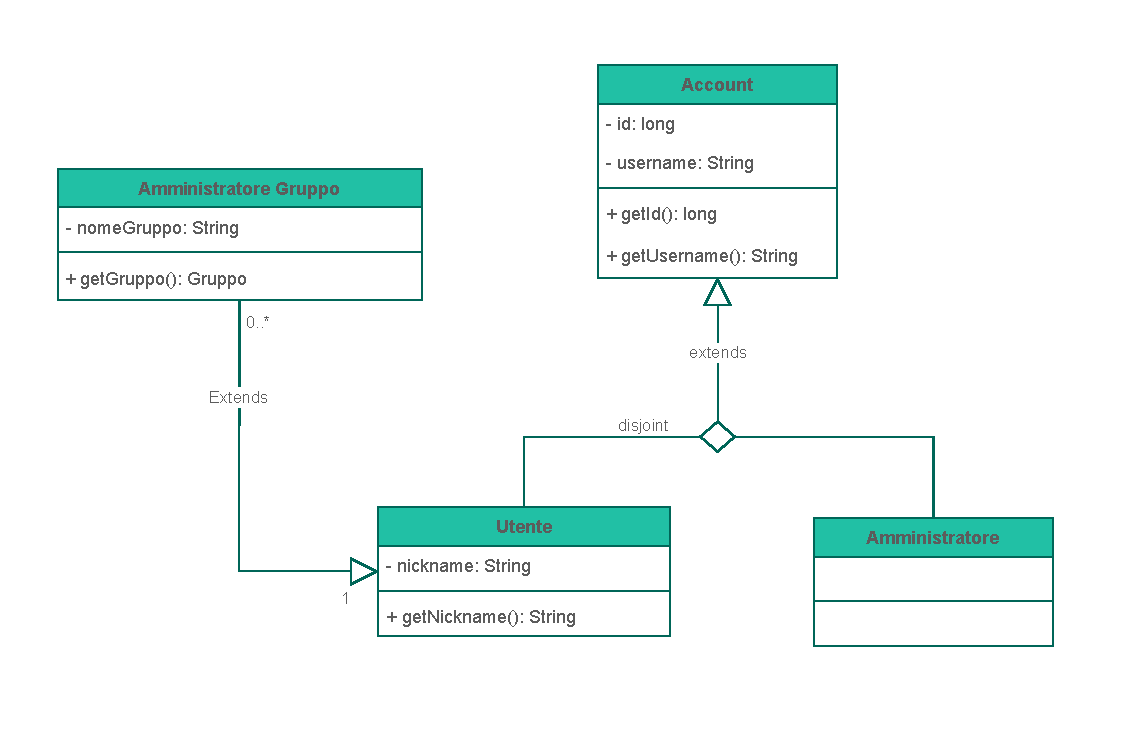
\includegraphics[scale=0.9]{progettazione/Progettazione-Struttura Account.drawio.pdf}
\end{adjustwidth}
\vspace{1cm}

\subsection*{Dominio: Amministrazione}
\phantomsection
\addcontentsline{toc}{subsection}{Dominio: Amministrazione}
\vspace{0.5cm}
\begin{adjustwidth}{-3.5cm}{0cm}
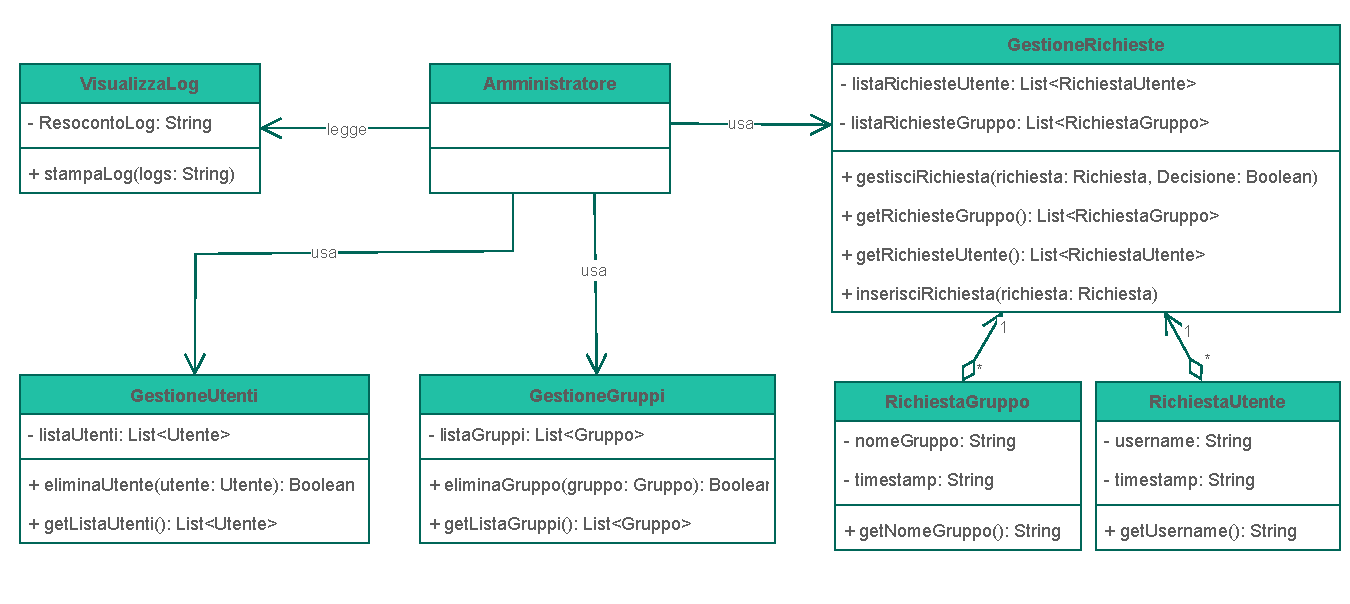
\includegraphics[scale=0.9]{progettazione/Progettazione-Amministrazione.drawio.pdf}
\end{adjustwidth}
\vspace{1cm}

\subsection*{Dominio: Area Personale}
\phantomsection
\addcontentsline{toc}{subsection}{Dominio: Area Personale}
\vspace{0.5cm}
\begin{adjustwidth}{-2cm}{0cm}
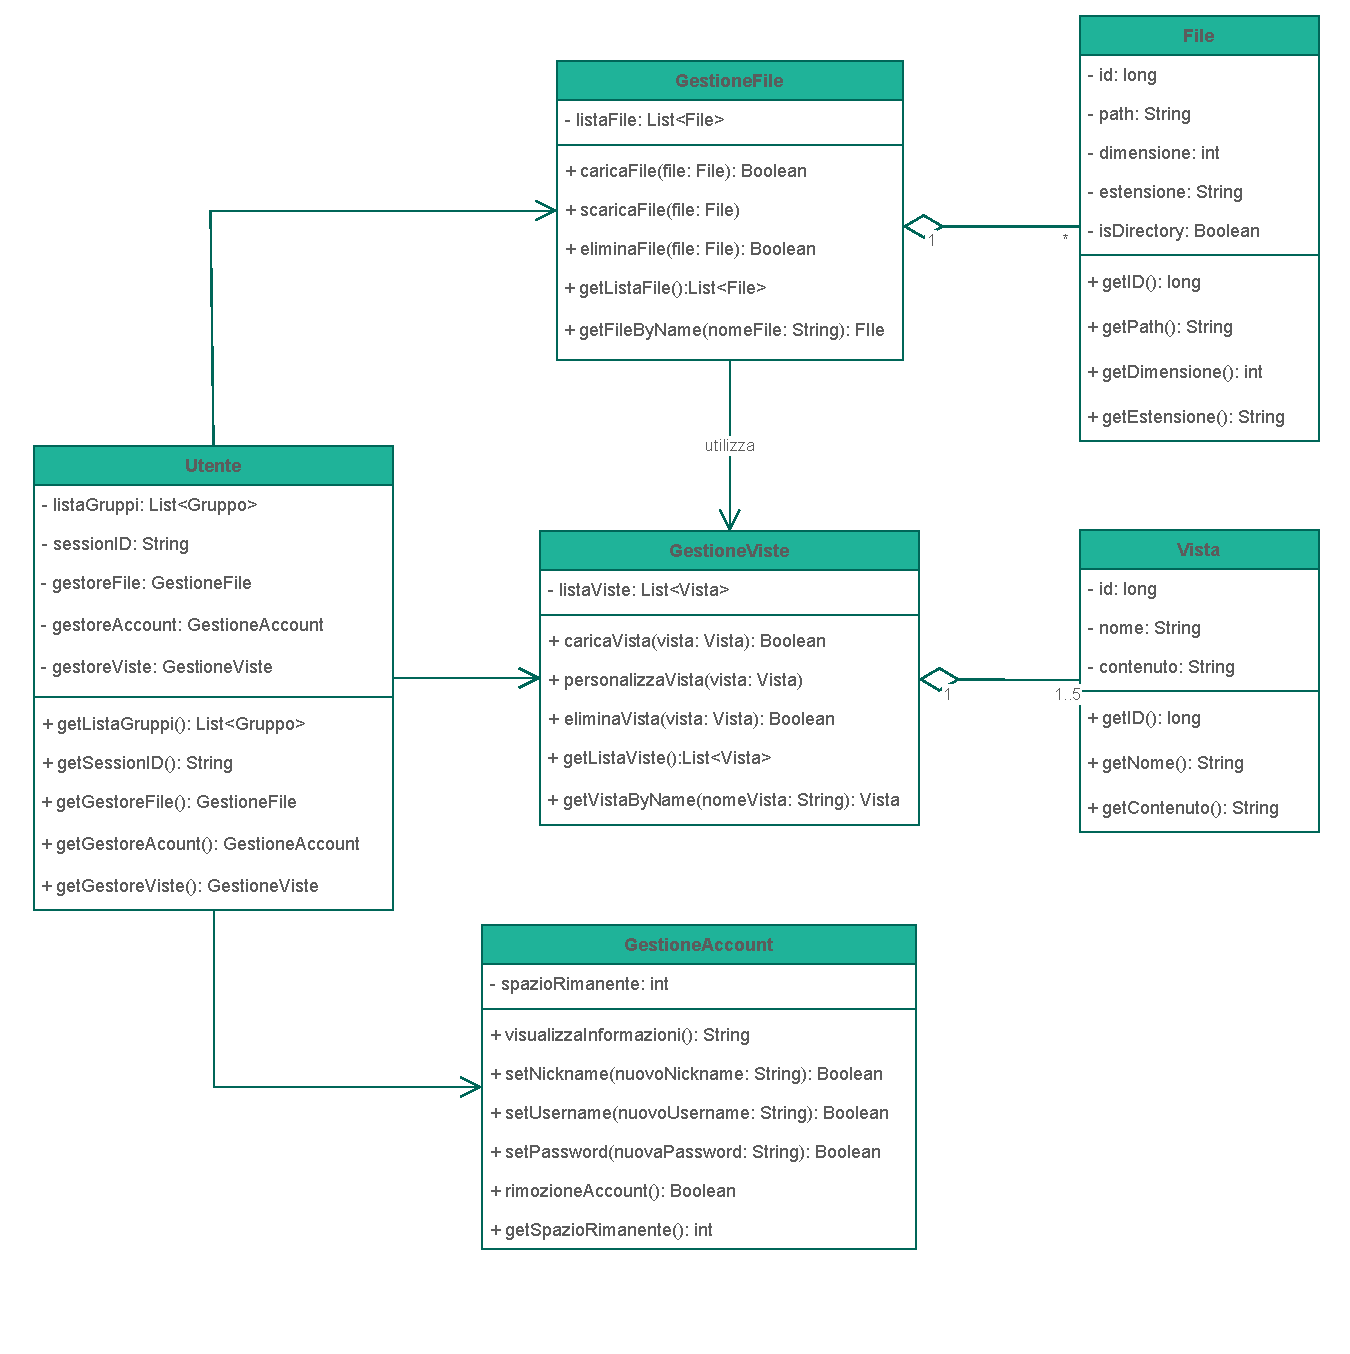
\includegraphics[scale=0.8]{progettazione/Progettazione-Area Personale.drawio.pdf}
\end{adjustwidth}
\vspace{1cm}
È stato deciso di creare una classe per i File, con un'istanza della classe per ogni File caricato dall'Utente.\\
Questo può essere oneroso per il Server in quanto occupa più memoria, però garantisce una migliore esperienza per l'Utente dato che l'accesso più facile all'alberatura dei file consente una navigazione più immediata.\\

\subsection*{Dominio: Area Gruppi}
\phantomsection
\addcontentsline{toc}{subsection}{Dominio: Area Gruppi}
\vspace{0.5cm}
\begin{adjustwidth}{-2cm}{0cm}
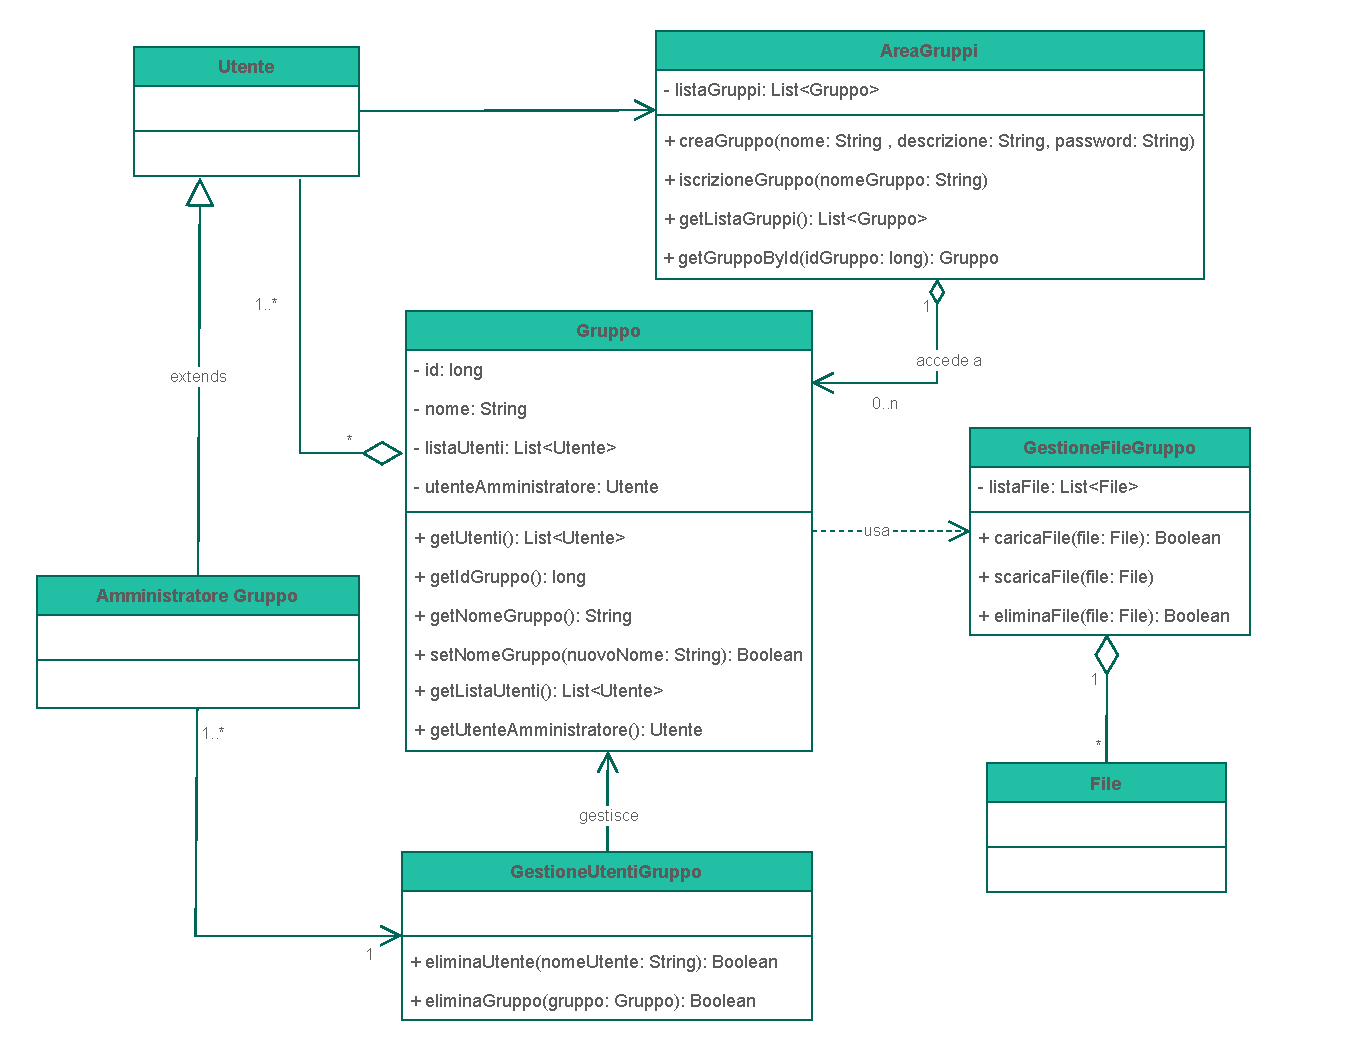
\includegraphics[scale=0.8]{progettazione/Progettazione-Area Gruppi.drawio.pdf}
\end{adjustwidth}
\vspace{1cm}


\subsection*{Diagramma di Dettaglio - Interfacce}
\phantomsection
\addcontentsline{toc}{subsection}{Interfacce}
\vspace{0.5cm}
\begin{adjustwidth}{-2.5cm}{0cm}
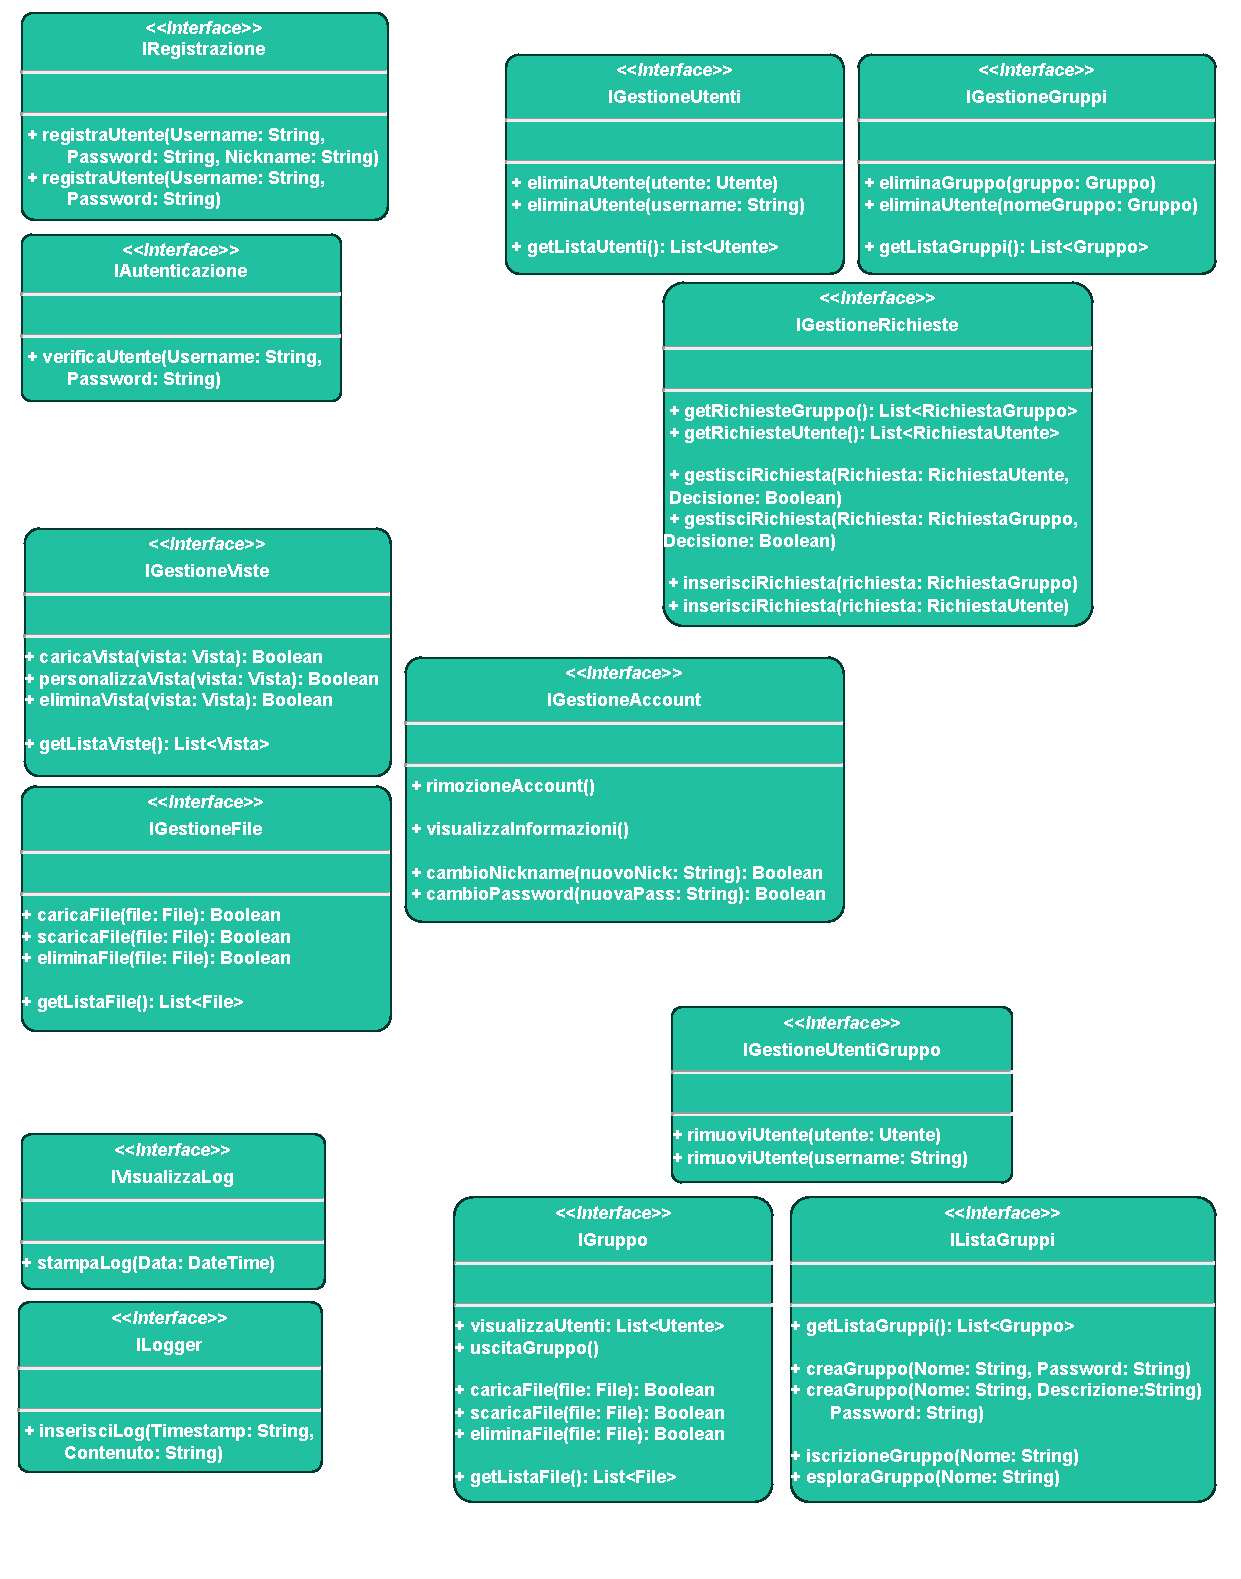
\includegraphics[scale=0.9]{progettazione/Progettazione-Interfacce.drawio.pdf}
\end{adjustwidth}
\vspace{1cm}


\subsection*{Diagramma di Dettaglio: Registrazione e Autenticazione}
\phantomsection
\addcontentsline{toc}{subsection}{Registrazione e Autenticazione}
\begin{adjustwidth}{-2cm}{0cm}
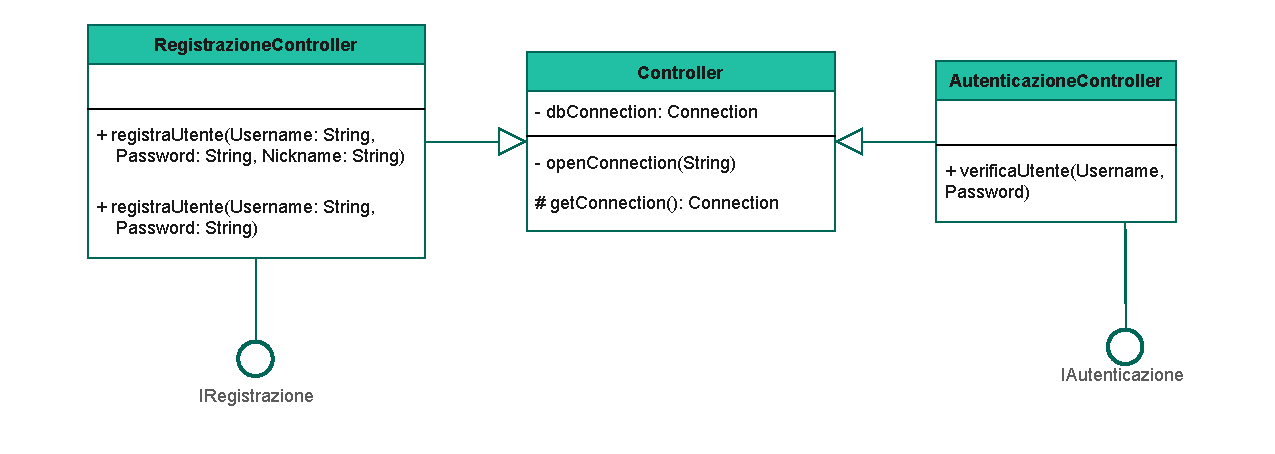
\includegraphics[scale=0.9]{progettazione/Progettazione-Dettaglio Autenticazione.drawio.pdf}
\end{adjustwidth}
\vspace{2cm}

\subsection*{Diagramma di Dettaglio: Amministrazione}
\phantomsection
\addcontentsline{toc}{subsection}{Amministrazione}
\begin{adjustwidth}{-3cm}{0cm}
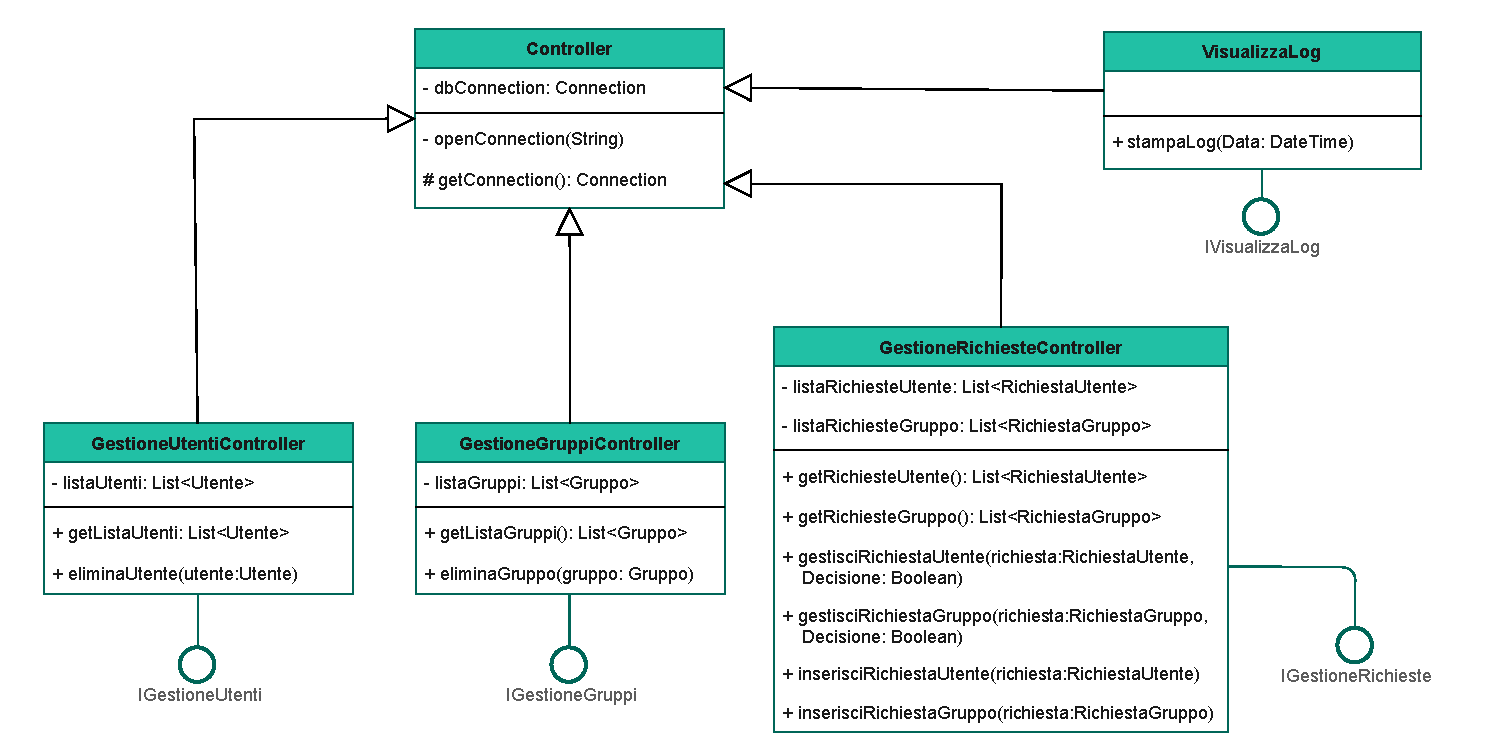
\includegraphics[scale=0.8]{progettazione/Progettazione-Dettaglio Amministratore.drawio.pdf}
\end{adjustwidth}
\vspace{0.5cm}


\subsection*{Diagramma di Dettaglio: Log}
\phantomsection
\addcontentsline{toc}{subsection}{Log}
\begin{adjustwidth}{-2cm}{0cm}
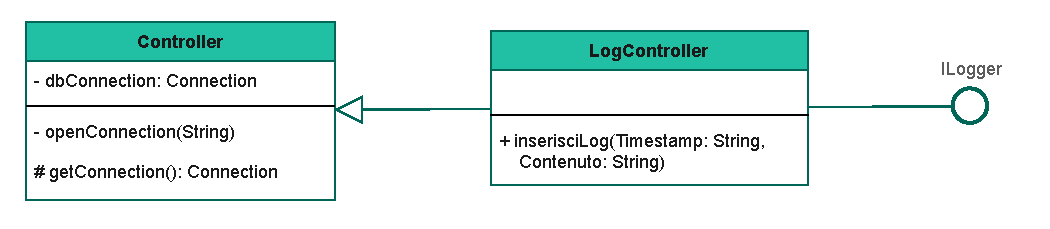
\includegraphics[scale=1]{progettazione/Progettazione-DettagliLog.drawio.pdf}
\end{adjustwidth}
\vspace{0.5cm}

\\
I Controller usano LogController per registrare ogni operazione come Log. A differenza delle altre classi, l'Amministratore può leggere i Log scritti dagli altri controller mediante VisualizzaLog.\\
\vspace{2cm}


\subsection*{Diagramma di Dettaglio: Utente}
\phantomsection
\addcontentsline{toc}{subsection}{Utente}
\vspace{0.5cm}
\begin{adjustwidth}{-1cm}{0cm}
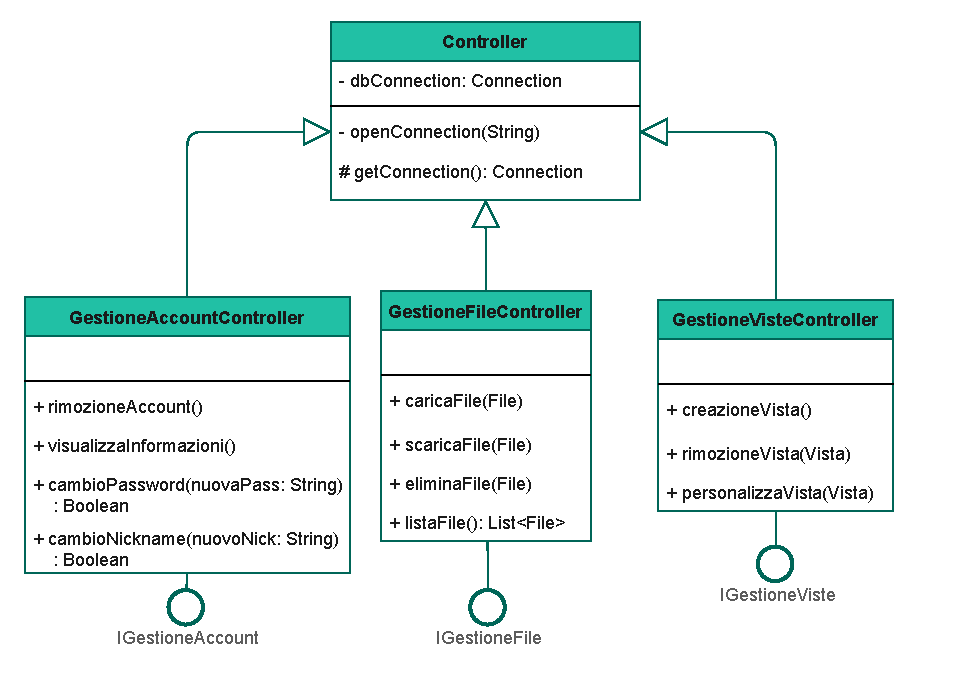
\includegraphics[scale=1]{progettazione/Progettazione-Dettaglio Utente.drawio.pdf}
\end{adjustwidth}
\vspace{0.5cm}

\subsection*{Diagramma di Dettaglio: Gruppi}
\vspace{0.5cm}
\phantomsection
\addcontentsline{toc}{subsection}{Gruppi}
\begin{adjustwidth}{-2cm}{0cm}
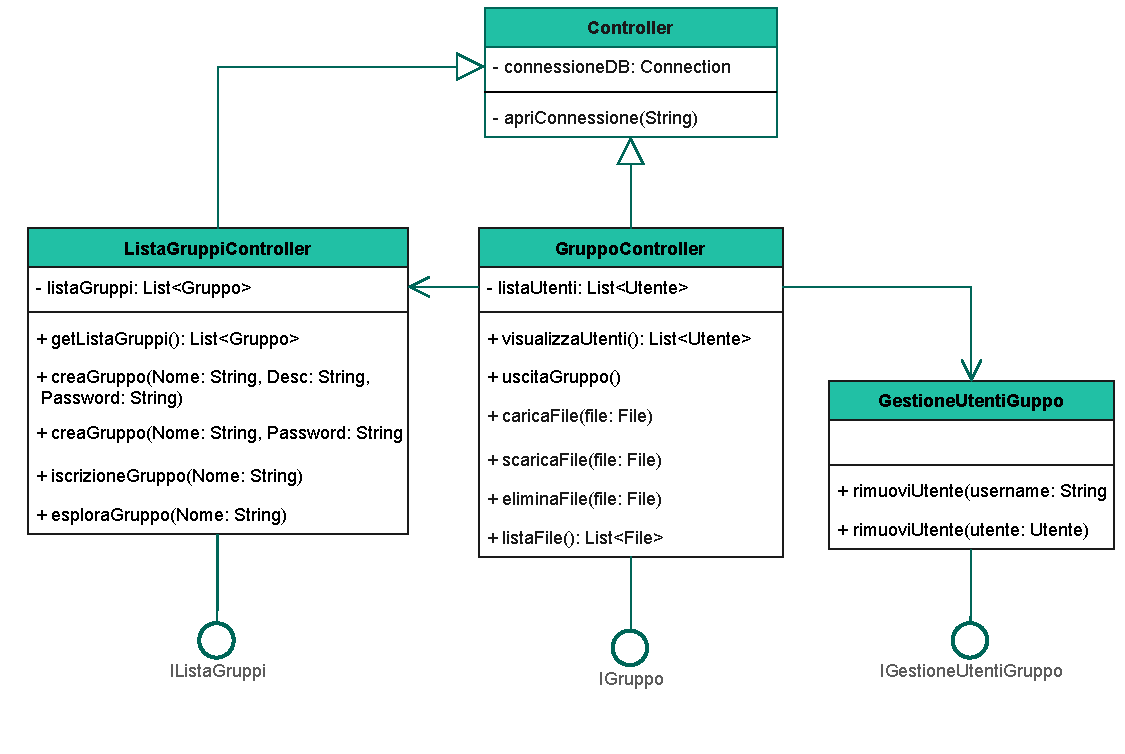
\includegraphics[scale=0.9]{progettazione/Progettazione-DettaglioGruppi.drawio.pdf}
\end{adjustwidth}
\vspace{0.5cm}



\pagebreak
\subsection*{Broker}
\phantomsection
\addcontentsline{toc}{subsection}{Broker}
Nel caso dell' applicazione web, il Broker può essere incorporato nel server web.
\\Così facendo possiamo delegare a quest'ultimo la capacità di gestire le richieste di connessione, catturando le sessioni dei clienti connessi e delegando a sua volta al Controller le operazioni necessarie per eseguire la registrazione e l'autenticazione.\\
Il Broker si interpone tra Client e Server e interagisce fin dalla prima connessione dell'utente al servizio. Potrà inoltre gestire molteplici richieste provenienti da numerosi utenti in parallelo, rendendo l'applicativo accessibile contemporaneamente nelle fasi di autenticazione.
Nel nostro caso specifico, il Broker è incorporato nel framework Dotnet. 
\vspace{0.5cm}



\subsection*{View di Registrazione e Autenticazione}
\phantomsection
\addcontentsline{toc}{subsection}{View di Registrazione e Autenticazione}
\begin{adjustwidth}{-2cm}{0cm}
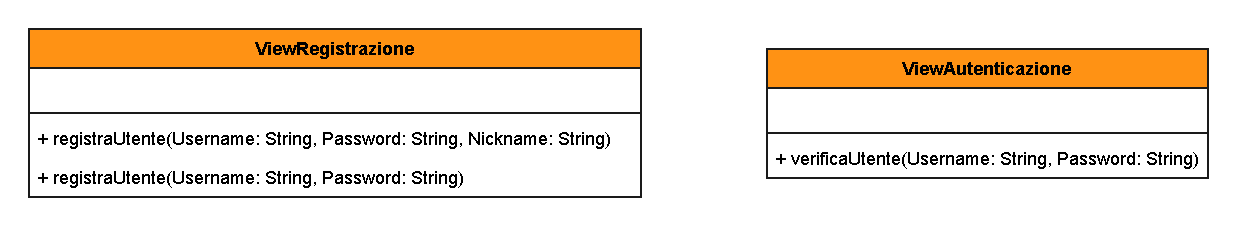
\includegraphics[scale=0.8]{progettazione/Progettazione-Interfacce Disponibili Registrazione_Autenticazione.drawio.pdf}
\end{adjustwidth}
\vspace{0.5cm}
\vspace{0.5cm}




\subsection*{View rese disponibili all' Utente}
\phantomsection
\addcontentsline{toc}{subsection}{View Utente}
\begin{adjustwidth}{-2cm}{0cm}
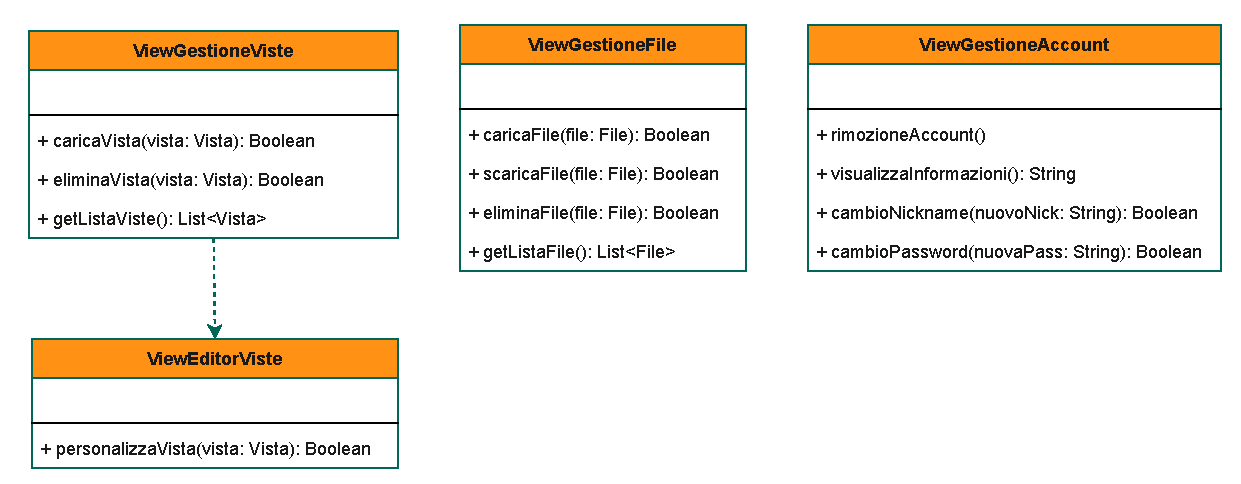
\includegraphics[scale=0.9]{progettazione/Progettazione-Interfacce Disponibili all' Utente.drawio.pdf}
\end{adjustwidth}
\vspace{0.5cm}
\vspace{0.5cm}


\subsection*{View rese disponibili ai Gruppi}
\phantomsection
\addcontentsline{toc}{subsection}{View Amministratore di Gruppo}
\begin{adjustwidth}{-3cm}{0cm}
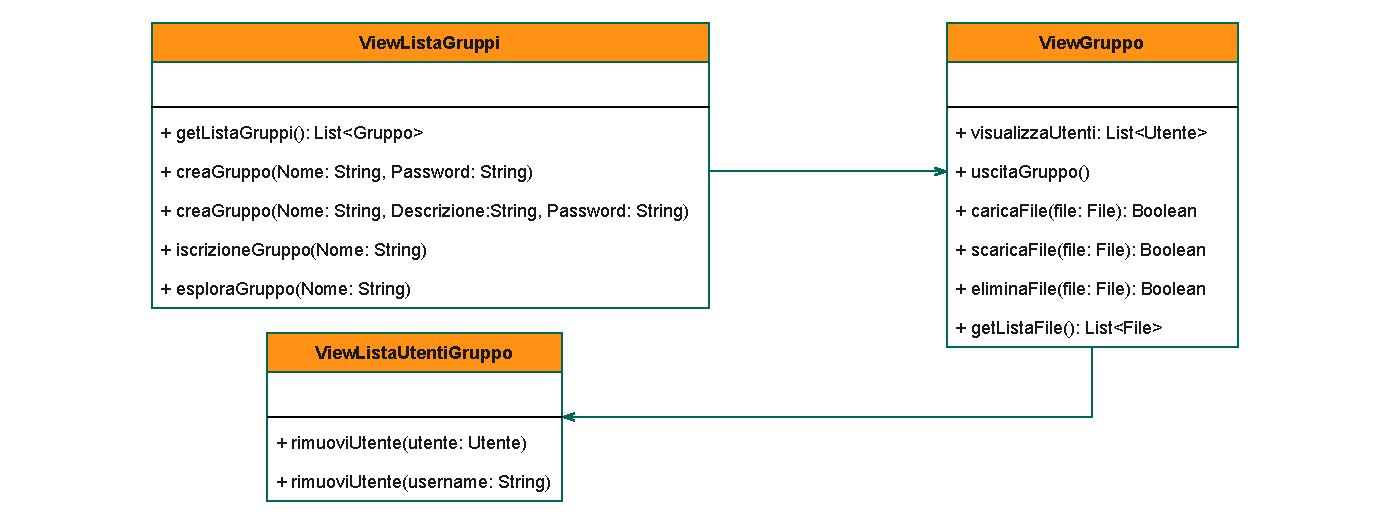
\includegraphics[scale=0.9]{progettazione/Progettazione-Interfacce Disponibili ai Gruppi.drawio.pdf}
\end{adjustwidth}
\vspace{0.5cm}


\subsection*{View rese disponibili all' Amministratore}
\phantomsection
\addcontentsline{toc}{subsection}{View Amministratore}
\begin{adjustwidth}{-2.5cm}{0cm}
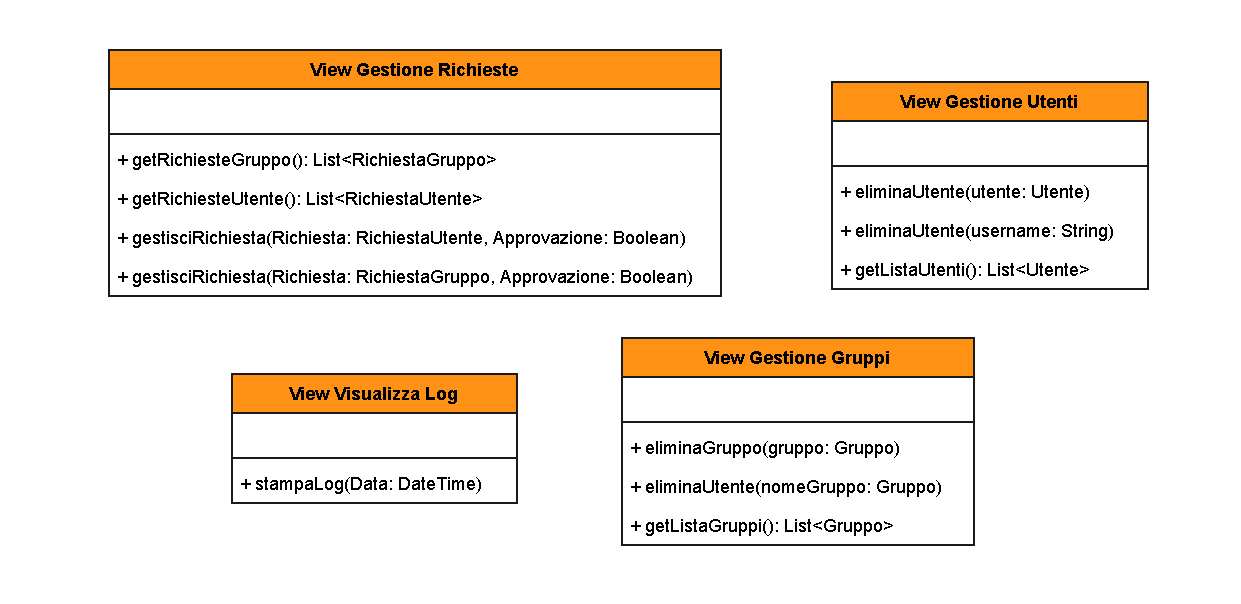
\includegraphics[scale=0.9]{progettazione/Progettazione-Interfacce Disponibili all' Amministratore.drawio.pdf}
\end{adjustwidth}
\vspace{0.5cm}



%----------------------------

\section*{Interfacce Applicazione}
\phantomsection
\addcontentsline{toc}{section}{Interfacce Applicazione}
\vspace{0.5cm}

\subsection*{Autenticazione}
\phantomsection
\addcontentsline{toc}{subsection}{Autenticazione}

\vspace{3cm}

\begin{adjustwidth}{-0.5cm}{0cm}
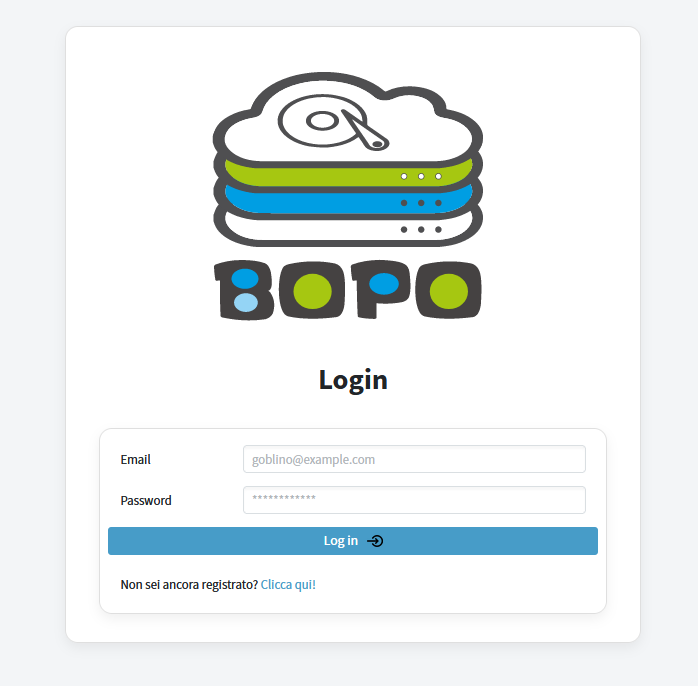
\includegraphics[scale=0.8]{figs/login.png}
\end{adjustwidth}
\pagecolor{background}\afterpage{\nopagecolor}



\subsection*{Registrazione}
\phantomsection
\addcontentsline{toc}{subsection}{Registrazione}
\vspace{3cm}
\begin{adjustwidth}{-0.5cm}{0cm}
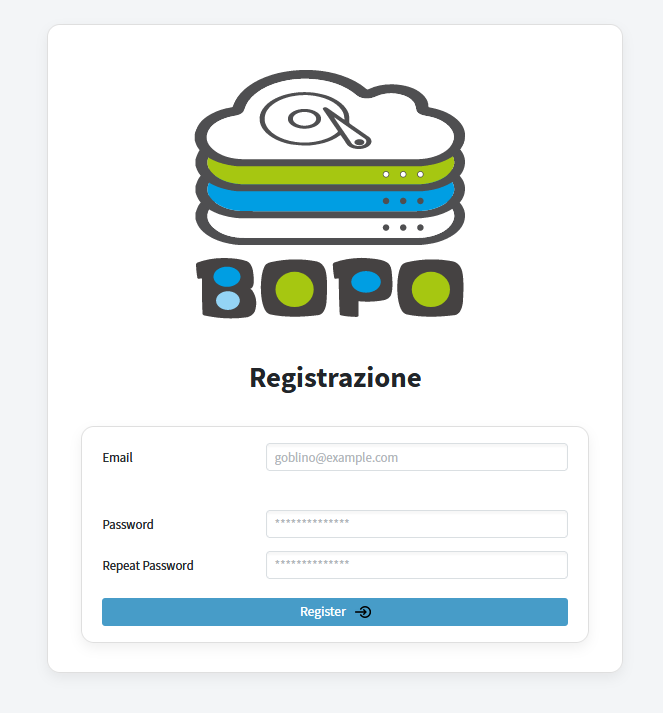
\includegraphics[scale=0.85]{figs/registrazione.png}
\end{adjustwidth}
\pagecolor{background}\afterpage{\nopagecolor}


\subsection*{Gestione Account}
\phantomsection
\addcontentsline{toc}{subsection}{Gestione Account}
\vspace{3cm}
\begin{adjustwidth}{-1.5cm}{0cm}
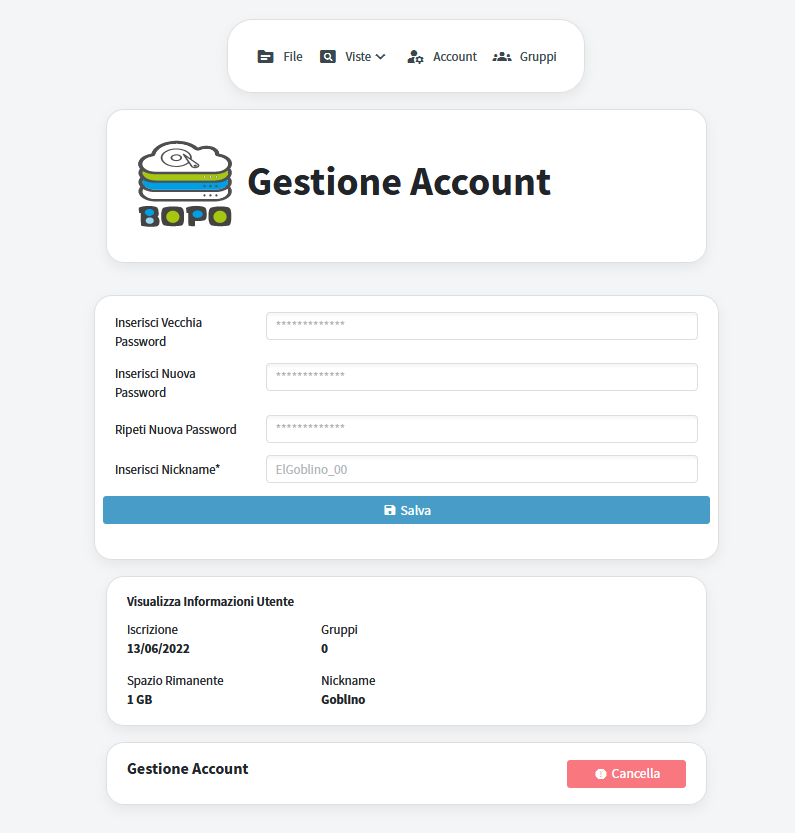
\includegraphics[scale=0.8]{figs/gestione_account.png}
\end{adjustwidth}
\pagecolor{background}\afterpage{\nopagecolor}



\subsection*{Gestione File}
\phantomsection
\addcontentsline{toc}{subsection}{Gestione File}
\vspace{3cm}
\begin{adjustwidth}{-4cm}{0cm}
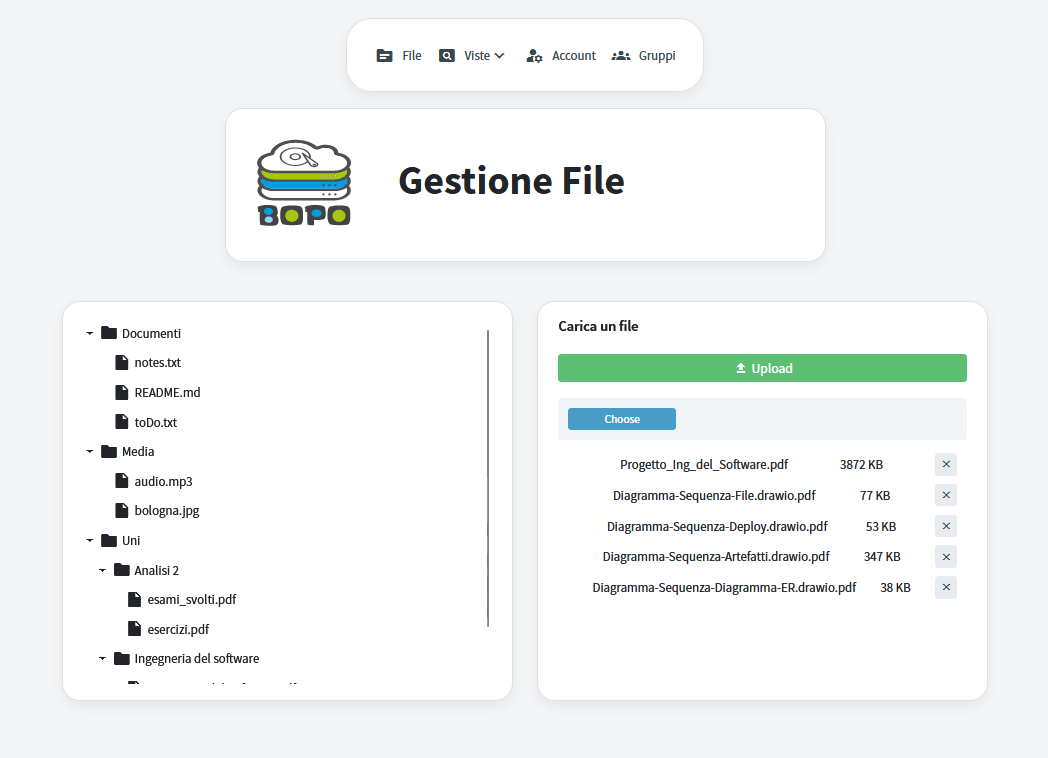
\includegraphics[scale=0.8]{figs/gestione_file.png}
\end{adjustwidth}
\pagecolor{background}\afterpage{\nopagecolor}


\subsection*{Gruppi}
\phantomsection
\addcontentsline{toc}{subsection}{Gruppi}
\vspace{3cm}
\begin{adjustwidth}{-3cm}{0cm}
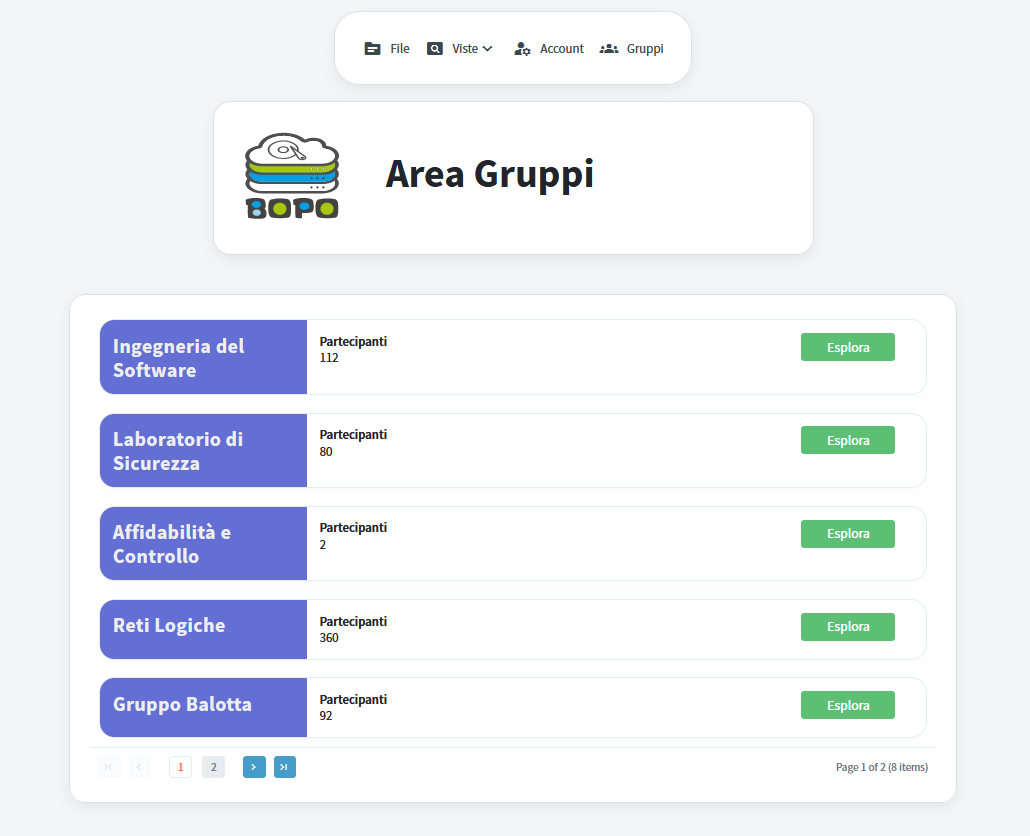
\includegraphics[scale=0.75]{figs/gruppi.png}
\end{adjustwidth}
\pagecolor{background}\afterpage{\nopagecolor}

%--------------------------------






\section*{Diagramma di dettaglio: Interazione}
\phantomsection
\addcontentsline{toc}{section}{Diagramma di dettaglio: Interazione}
\vspace{0.5cm}



\subsection*{Diagramma di Sequenza: Registrazione}
\phantomsection
\addcontentsline{toc}{subsection}{Diagramma di Sequenza: Registrazione}
\vspace{2cm}
\begin{adjustwidth}{-2cm}{0cm}
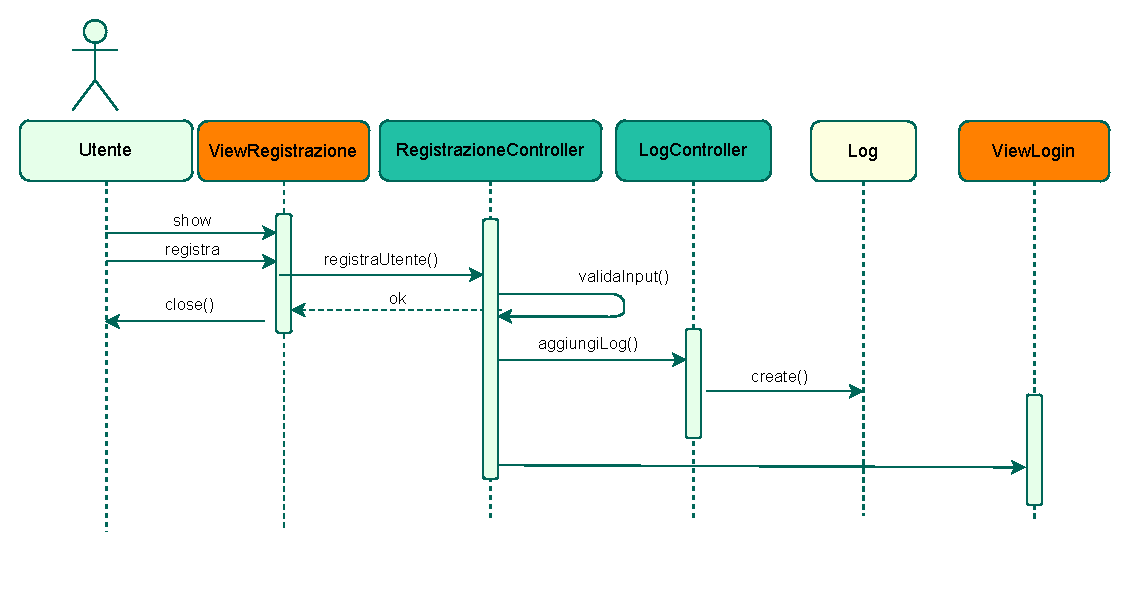
\includegraphics[scale=0.9]{progettazione/Diagramma-Sequenza-Interazione-Registrazione.drawio.pdf}
\end{adjustwidth}
\vspace{0.5cm}
Nella fase di registrazione, l'Utente non interroga direttamente il database. La richiesta deve essere approvata in primo luogo dall' Amministratore, il quale avrà i metodi delegati alla connessione e interrogazione del database dei dati degli Utenti.
Ogni tentativo di autenticazione viene registrato in un altro database che mantiene in modo persistente i Log di sistema.

\subsection*{Diagramma di Sequenza: Autenticazione}
\phantomsection
\addcontentsline{toc}{subsection}{Diagramma di Sequenza: Autenticazione}
\vspace{2cm}
\begin{adjustwidth}{-2cm}{0cm}
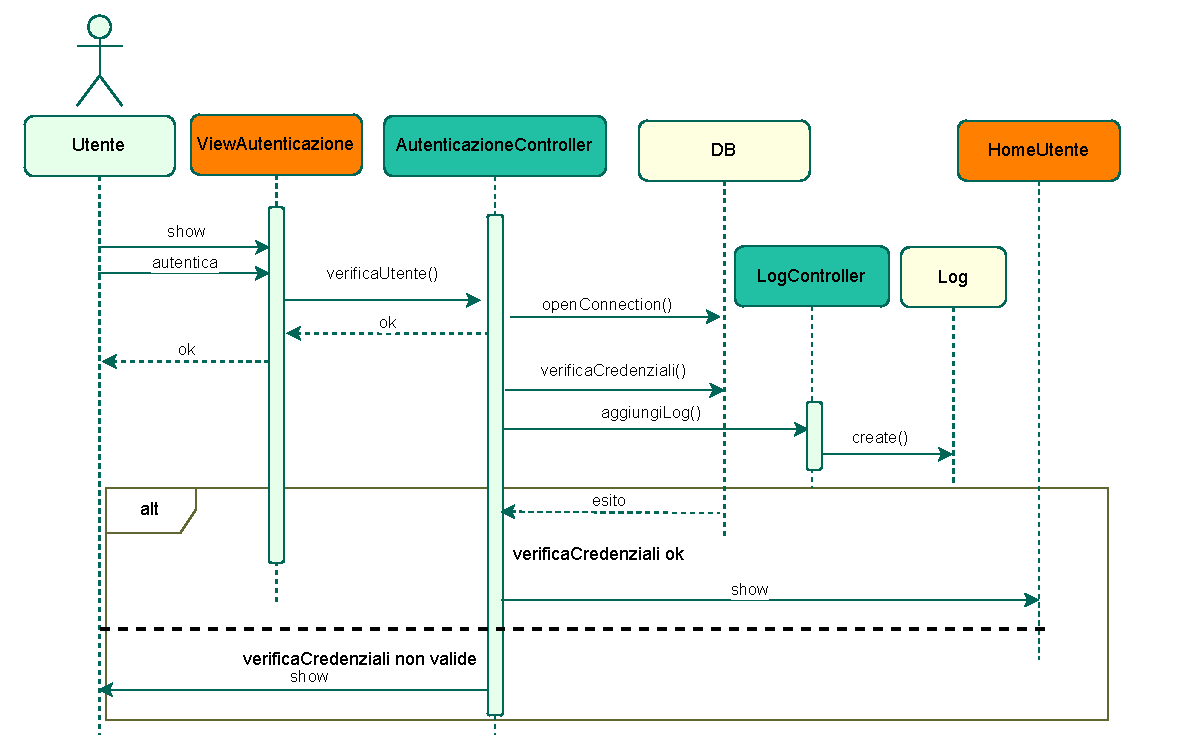
\includegraphics[scale=0.9]{progettazione/Diagramma-Sequenza-Interazione-Autenticazione.drawio.pdf}
\end{adjustwidth}
\vspace{0.5cm}
La fase di autenticazione inserisce i log nel database della persistenza in ogni tentativo di autenticazione. Nel Login si interroga invece il database dei dati degli Utenti.

\subsection*{Diagramma di Sequenza: Gestione Amministratore}
\phantomsection
\addcontentsline{toc}{subsection}{Diagramma di Sequenza: Gestione Amministratore}
\begin{adjustwidth}{-1cm}{0cm}
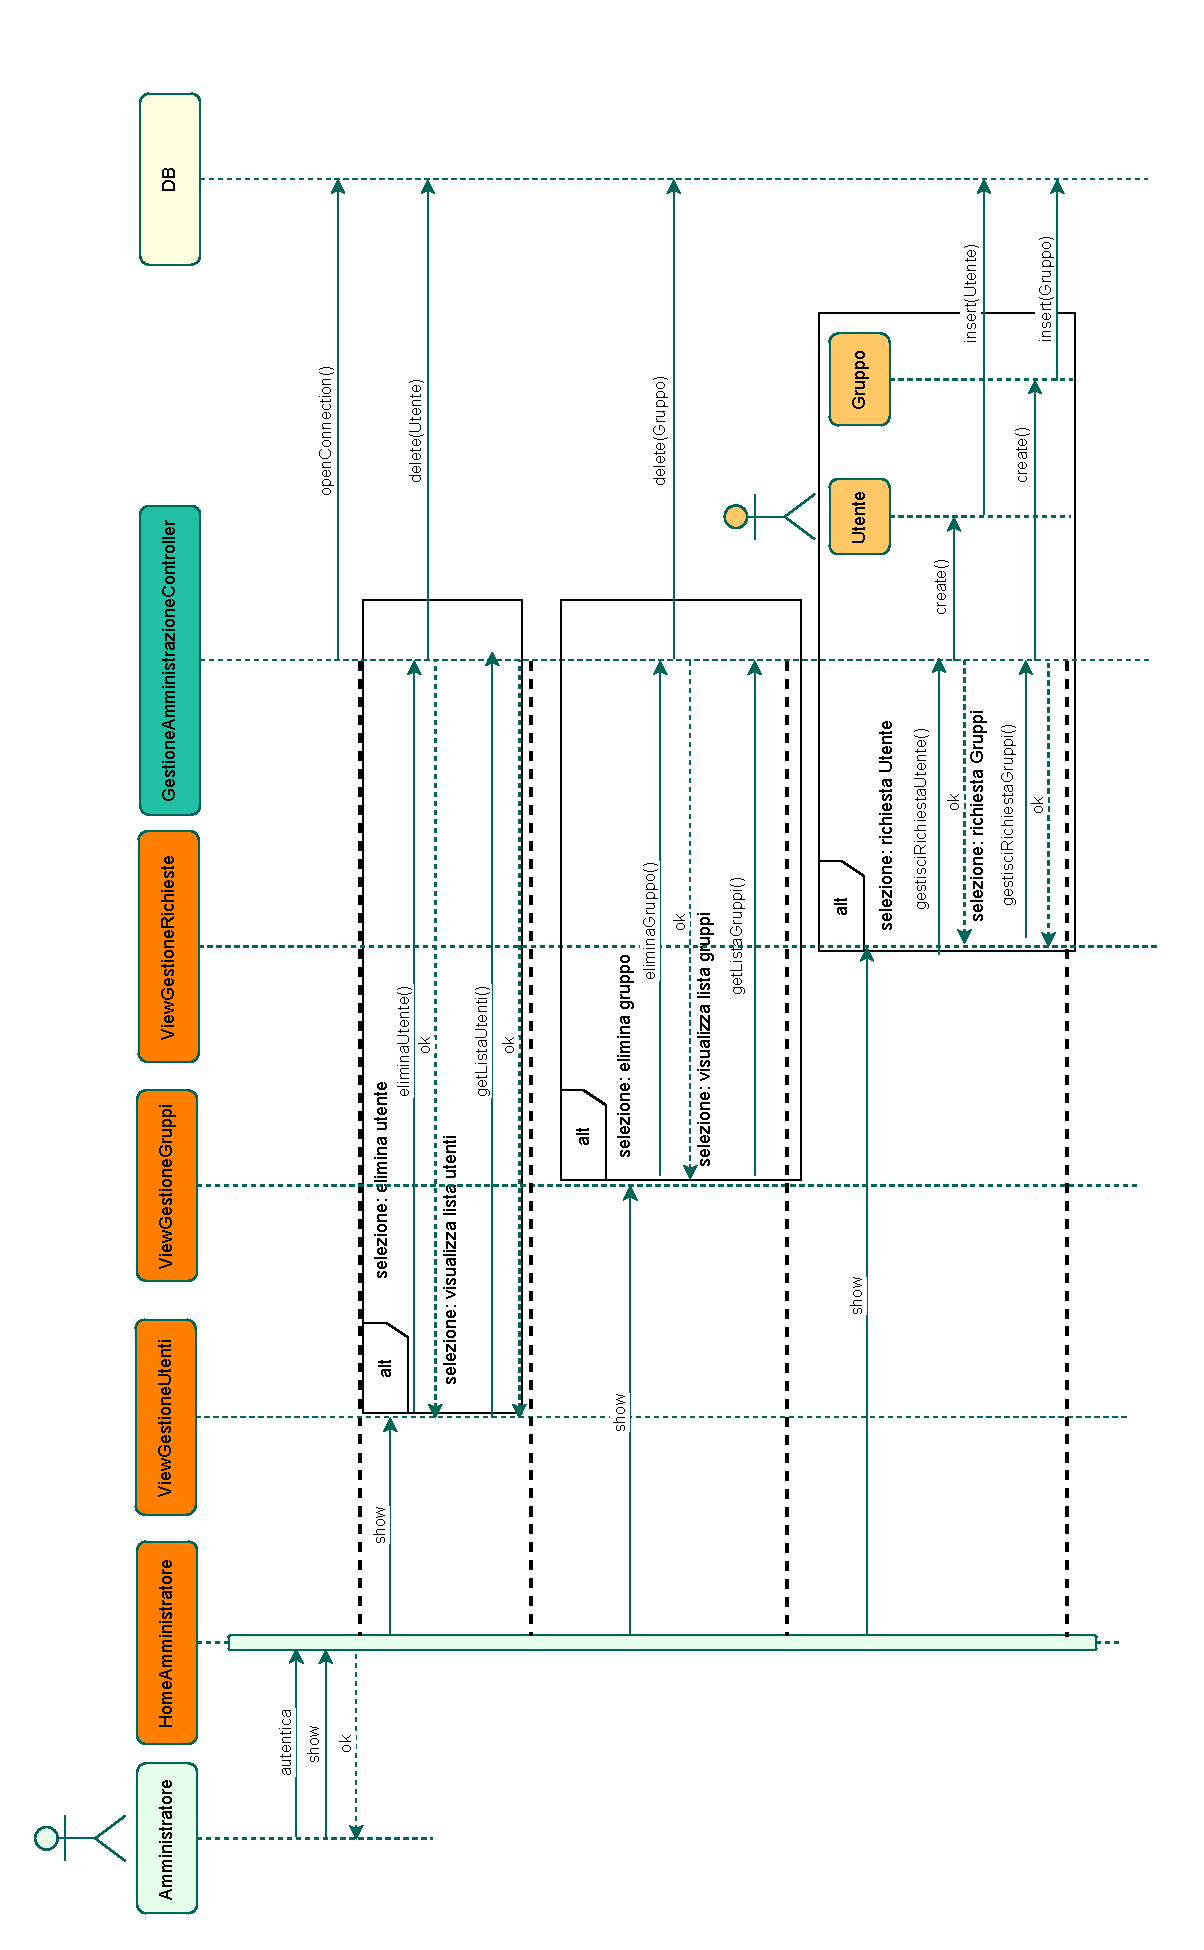
\includegraphics[scale=0.75]{progettazione/Diagramma-Sequenza-Interazione-GestioneAmministratore.drawio.pdf}
\end{adjustwidth}
\vspace{0.5cm}
L'Amministratore ha il ruolo di accettare la coda di richieste provenienti dagli Utenti e dai Gruppi. Si distinguono in questa fase le richieste dell' Utente da quelle del Gruppo. Dopo l'accettazione di una delle due richieste, si raggiungerà lo stesso database Utente/Gruppo in cui verranno registrate le nuove informazioni scatenate dalla richiesta.



\subsection*{Diagramma di Sequenza: Interazione Area Personale\-Viste}
\phantomsection
\addcontentsline{toc}{subsection}{Diagramma di Sequenza: Interazione Area Personale\-Viste}
\begin{adjustwidth}{-2.5cm}{0cm}
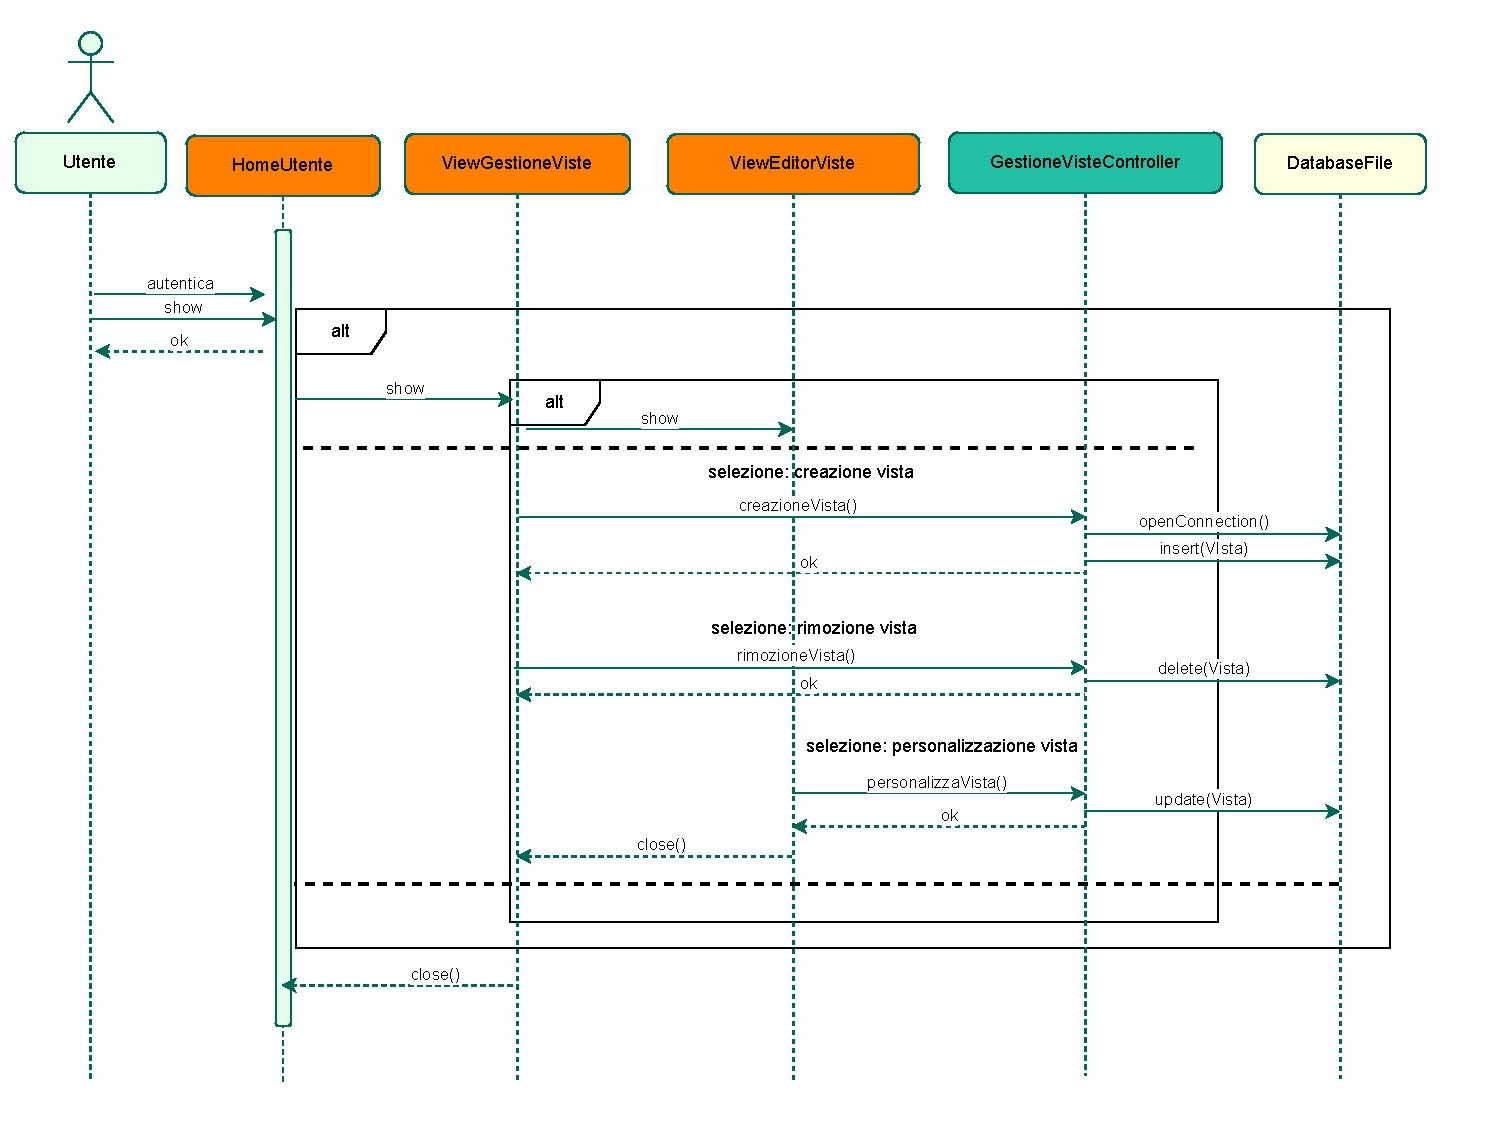
\includegraphics[scale=0.8]{progettazione/Diagramma-Sequenza-Interazione-Viste.drawio.pdf}
\end{adjustwidth}
\vspace{0.5cm}


\subsection*{Diagramma di Sequenza: Interazione Area Gruppi}
\phantomsection
\addcontentsline{toc}{subsection}{Diagramma di Sequenza: Interazione Area Gruppi}
\begin{adjustwidth}{-1.5cm}{0cm}
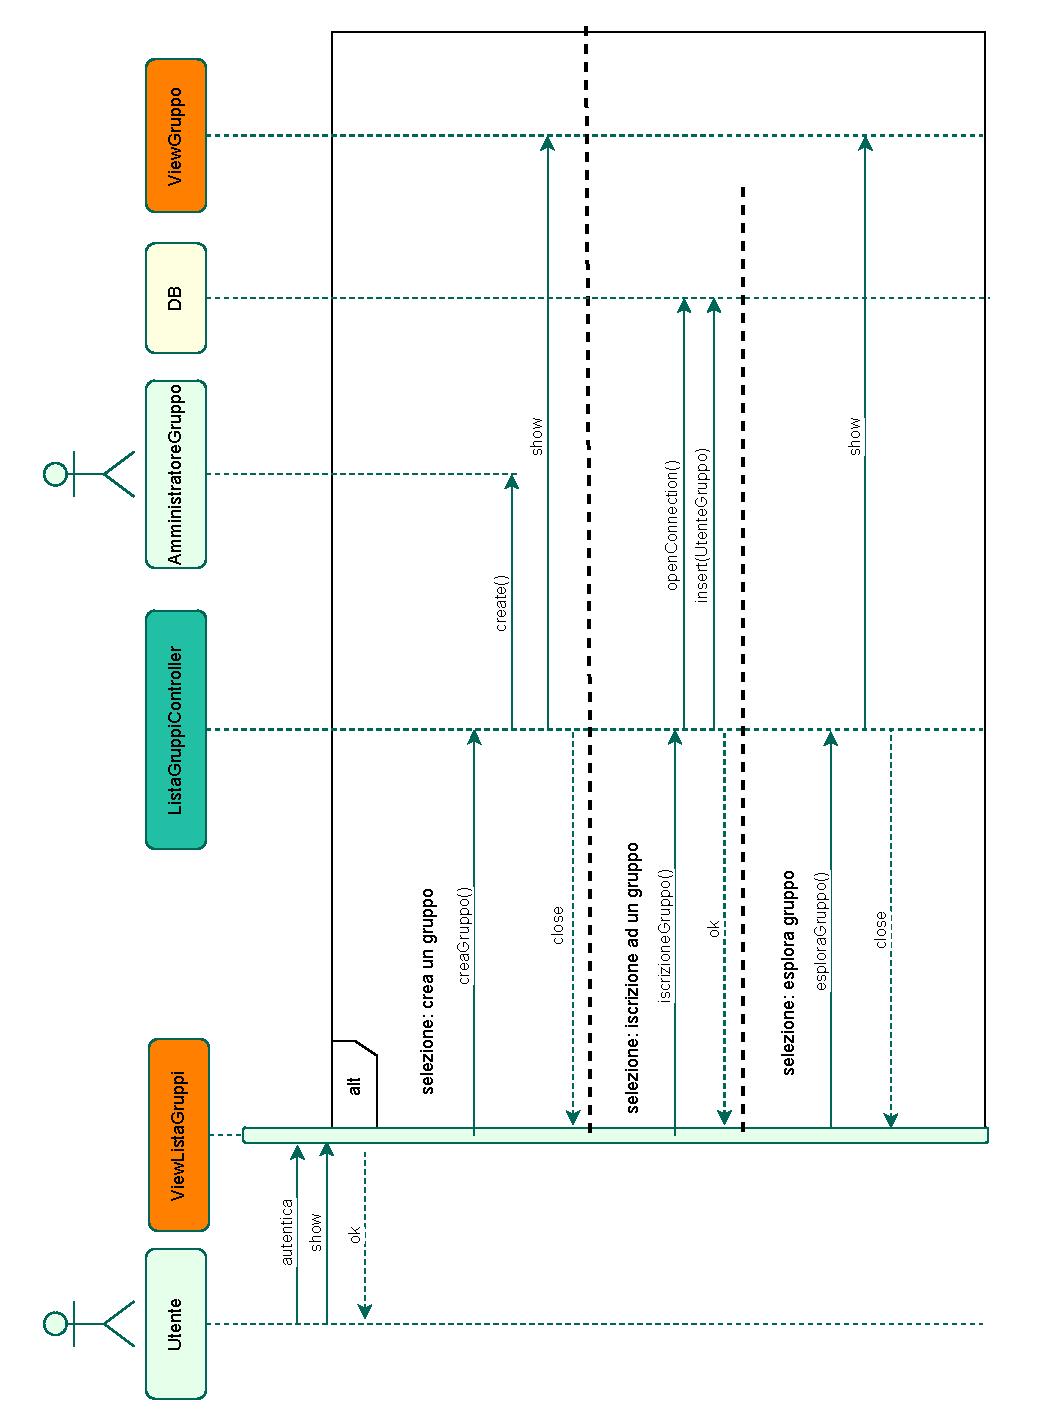
\includegraphics[scale=0.95]{progettazione/Diagramma-Sequenza-Interazione-AreaGruppi.drawio.pdf}
\end{adjustwidth}
\vspace{0.5cm}


\subsection*{Diagramma di Sequenza: Interazione Log}
\phantomsection
\addcontentsline{toc}{subsection}{Diagramma di Sequenza: Interazione Log}
\vspace{1.5cm}
\begin{adjustwidth}{0cm}{0cm}
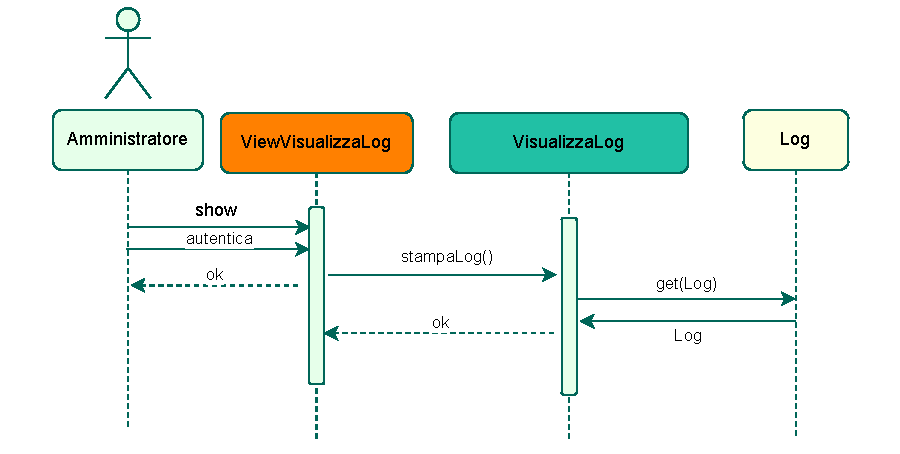
\includegraphics[scale=1]{progettazione/Diagramma-Sequenza-Interazione-Log.drawio.pdf}
\end{adjustwidth}
\vspace{0.5cm}


%---------------------------------------------------------


\pagebreak
\section*{Progettazione Persistenza}
\phantomsection
\addcontentsline{toc}{section}{Progettazione Persistenza}
\vspace{1cm}
La persistenza del \verb|DatabaseUtentiGruppi| verrà implementata utilizzando un DBMS, in particolare MariaDB.
\vspace{0.5cm}
\subsection*{Diagramma Entity-Relation}
\phantomsection
\addcontentsline{toc}{subsection}{Diagramma E-R}
\vspace{0.5cm}
\begin{adjustwidth}{-2cm}{0cm}
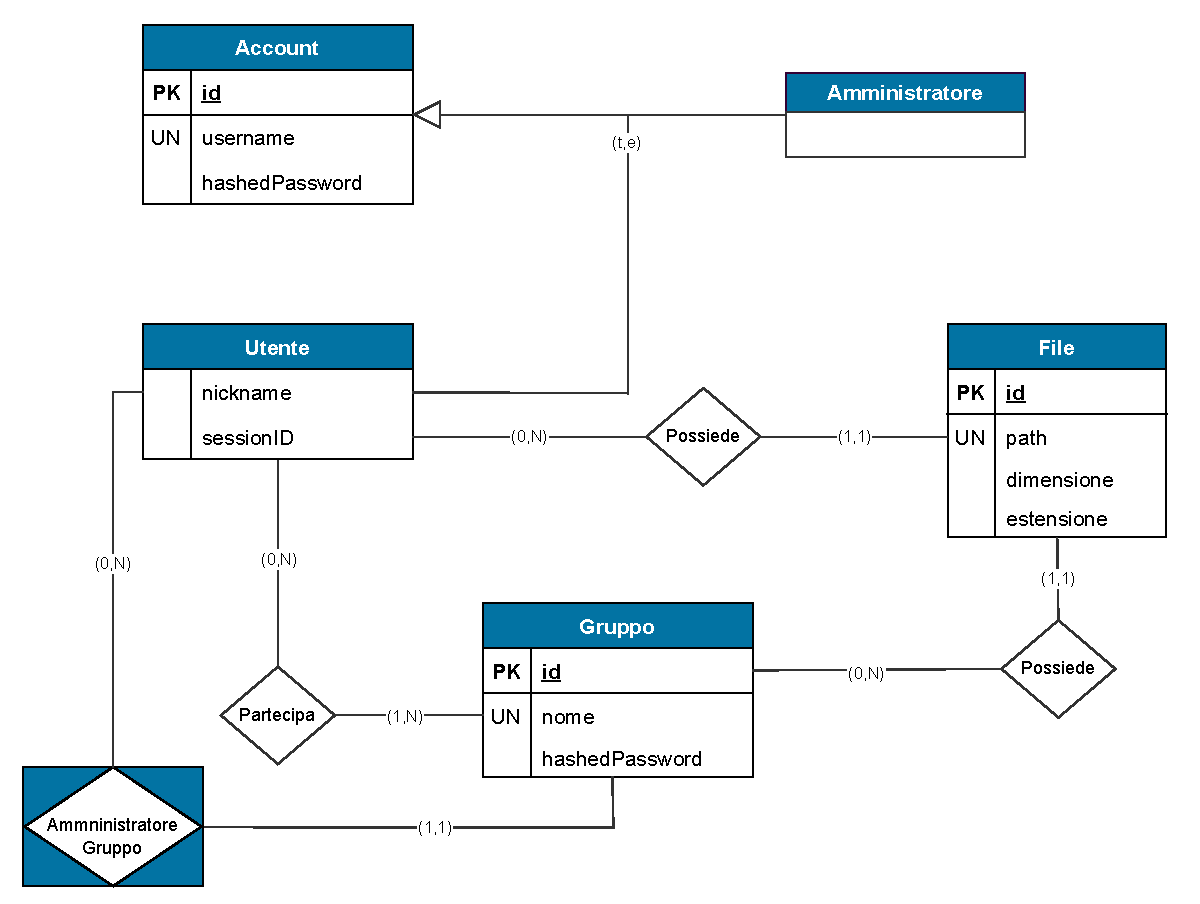
\includegraphics[scale=0.9]{progettazione/Diagramma-Sequenza-Diagramma-ER.drawio.pdf}
\end{adjustwidth}
\vspace{0.5cm}


\vspace{1cm}
\subsection*{Persistenza File}
\phantomsection
\addcontentsline{toc}{subsection}{Persistenza File}
\vspace{0.5cm}
\begin{adjustwidth}{-1cm}{0cm}
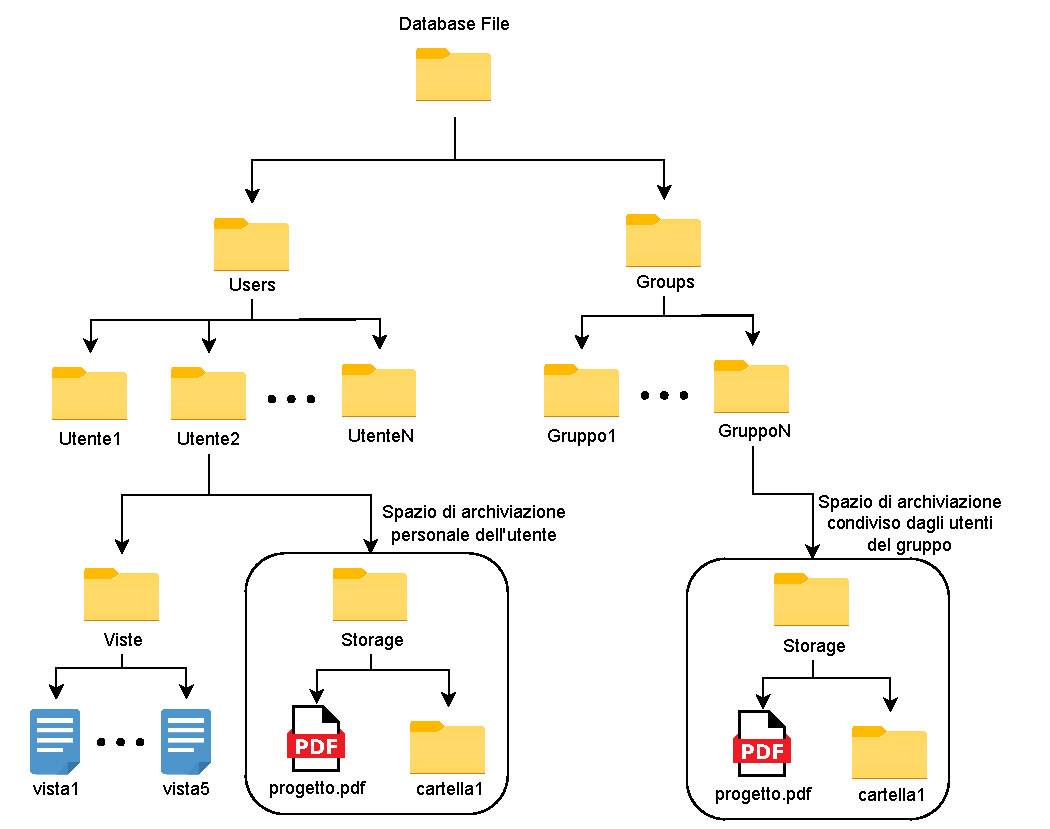
\includegraphics[scale=1]{deployment/Diagramma-Sequenza-File.drawio.pdf}
\end{adjustwidth}
\vspace{0.5cm}

\phantomsection
\addcontentsline{toc}{subsection}{Formato Log}
\vspace{0.5cm}


\subsection*{Formato Log}
I file di Log vengono memorizzati giornalmente attraverso il DatabaseLog. Ogni giorno viene generato un nuovo file così da tener traccia degli accessi al sistema e degli eventi.\\
\\
Ogni entry rispetta questo formato:\\

    \begin{tabular}{|p{3cm} p{3cm} p{3cm}|}
    \hline
    \verb |yyyy-mm-dd-hh-mm| & : \verb|event| & : \verb|data|\\
    \hline
    Timestamp   & Evento che ha generato il Log & Contenuto del Log \\
    \hline
    \end{tabular}
    
    
    
\pagebreak
\section*{Progettazione Collaudo}
\phantomsection
\addcontentsline{toc}{section}{Progettazione Collaudo}
\vspace{1cm}

\inputminted
[
frame=lines,
framesep=2mm,
baselinestretch=1.2,
bgcolor=opal!20!,
fontsize=\footnotesize,
linenos
]
{csharp}{code/collaudo.cs}
%----------------------------------------


\pagebreak
\section*{Deployment}
\phantomsection
\addcontentsline{toc}{section}{Deployment}
\subsection*{Artefatti}
\vspace{1cm}
\phantomsection
\addcontentsline{toc}{subsection}{Artefatti}
\vspace{0.5cm}
\begin{adjustwidth}{0cm}{0cm}
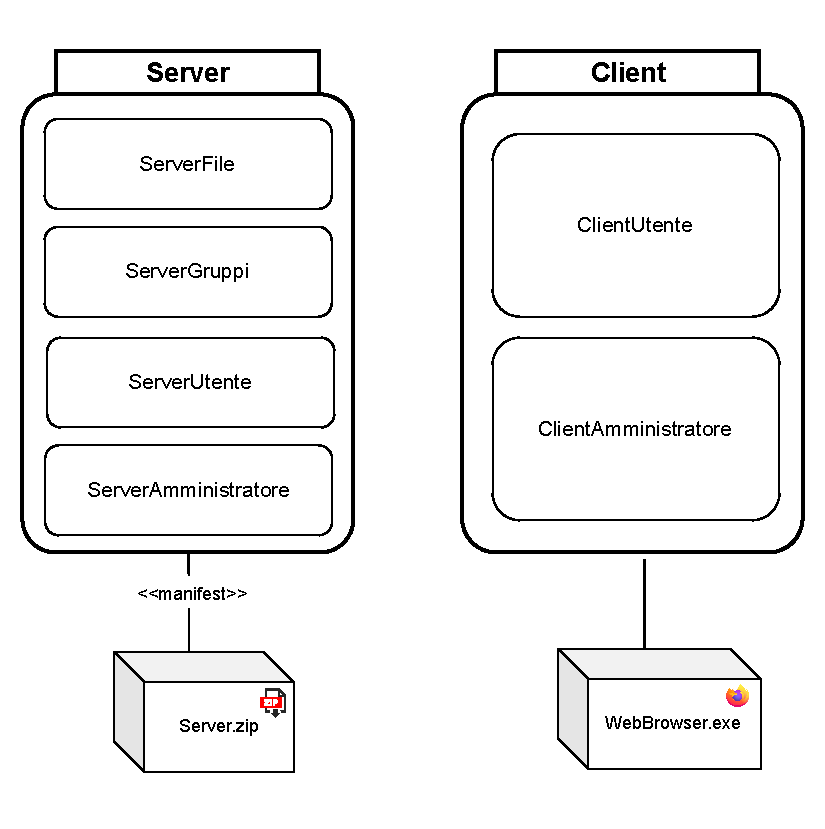
\includegraphics[scale=1]{deployment/Diagramma-Sequenza-Artefatti.drawio.pdf}
\end{adjustwidth}

\vspace{1cm}
\subsection*{Deploy}
\phantomsection
\addcontentsline{toc}{subsection}{Deploy}
\vspace{0.5cm}
\begin{adjustwidth}{-3cm}{0cm}
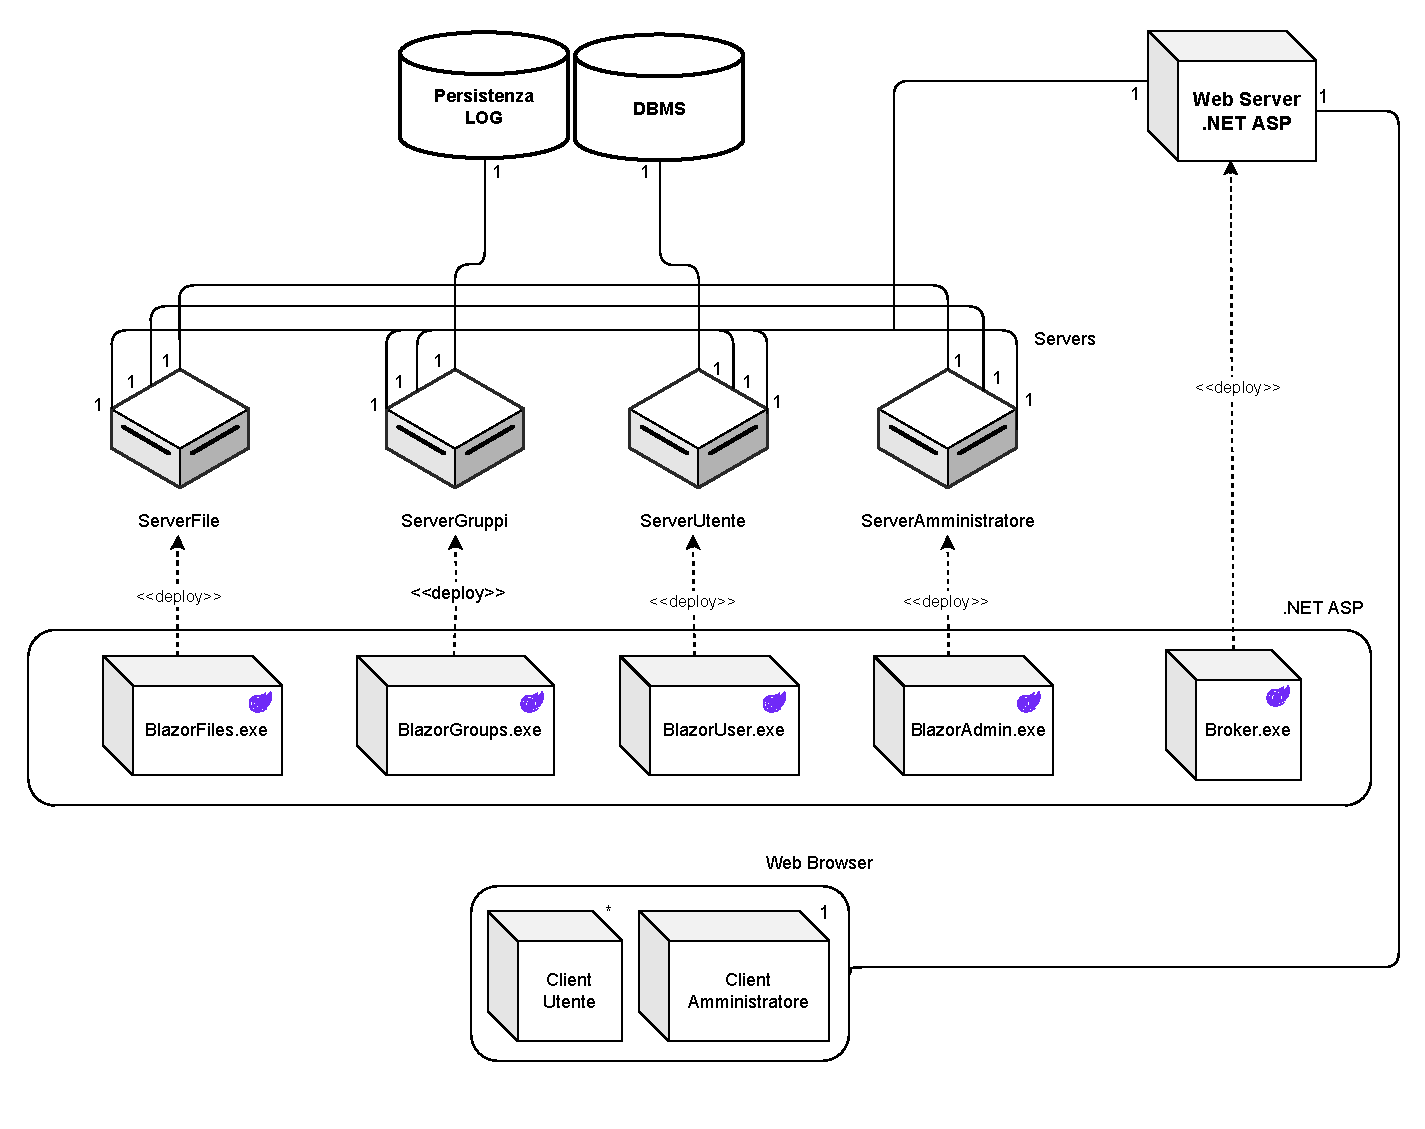
\includegraphics[scale=0.8]{deployment/Diagramma-Sequenza-Deploy.drawio.pdf}
\end{adjustwidth}

\end{document}
